\documentclass[lang=cn,12pt,math=newtx,thmcnt=section,chinesefont=founder]{vavidbook}
% 环境设置

%% 宏包
% 颜色包
\usepackage{soul, color}

% 箭头选项
\usepackage{extarrows}

% 表格 `diagbox`(斜对角线)
\usepackage{array, tabularx, tabularray, longtable, diagbox}

% 消除警告
\usepackage{silence}
% 支持插入动画
\usepackage{animate}

% 子图 浮动体 虚线
\makeatletter
\let\c@lofdepth\relax
\let\c@lotdepth\relax
\makeatother
\usepackage{subfigure, float, arydshln}

% 超链接和目录
\usepackage{tocbibind}
\usetikzlibrary{arrows.meta}
\usetikzlibrary{patterns}

% 图片路径
\graphicspath{{./figure/Cover/},{./figure/Note/}}

% 封面设置
\title{\LaTeX\quad \quad \textbf{\textit{main}}} % 标题
\subtitle{{\fontspec{Times New Roman}\textit{Sun for morning, moon for night, and you forever.}}} % 副标题
\author{Lyshmily.Y \& 木易} % 作者
\institute{Lyshmily.Y} % 机构
\date{\today} % 日期
\version{V.1.0} % 版本
\bioinfo{邮箱}{\email{yjlpku.outlook.com} \& \email{845307723@qq.com}} % 信息
\extrainfo{在没有结束前,总要做很多没有意义的事,这样才可以在未来某一天,用这些无意义的事去堵住那些讨厌的缺口} % 箴言
\logo{pku.jpg} % 徽标
\cover{coverc.jpg} % 封面

%% 设置
\setcounter{tocdepth}{3} % 目录深度
\renewcommand{\arraystretch}{1.2} % 表格行高

%% 自定义命令
\def\d{\textup{d}} % 直立体 d 用于微分符号 dx
\def\artanh{\operatorname{artanh}}  % 定义artanh函数
\def\arsinh{\operatorname{arsinh}}  % 定义arsinh函数
\def\arcosh{\operatorname{arcosh}}  % 定义arcosh函数

% 指定颜色的数学公式框
\newcommand{\mathcolorbox}[2]{\colorbox{#1}{$\displaystyle #2$}}
% 空行 \myspace{n}
\newcommand{\myspace}[1]{\par\vspace{#1\baselineskip}}
% 大小写罗马数字 \Rmnum{n} \rmnum{n}
\makeatletter
\newcommand{\rmnum}[1]{\romannumeral #1}
\newcommand{\Rmnum}[1]{\expandafter\@slowromancap\romannumeral #1@}
\makeatother

\begin{document}
	% 封面
	\maketitle
	% 目录
	\chapterimage{目录.jpg}
	%\tableofcontents
	\mainmatter
	% 正文
	\chapterimage{chap1.jpg}
\chapter{绪论}
\section{数据结构}
\begin{definition}[基本术语]
    \begin{enumerate}
        \item 数据: 描述客观事物的符号, 是计算机中可以操作的对象, 是计算机中的输入和输出的信息
        \item 数据元素: 是数据的基本单位, 在计算机中通常作为一个整体进行考虑和处理
        \item 数据项: 一个数据元素可以由若干个数据项组成, 数据项是数据不可分割的最小单位
        \item 数据结构: 是相互之间存在一种或多种特定关系的数据元素的集合
        \item 数据对象: 是具有相同性质的数据元素的集合, 是数据的子集
    \end{enumerate}
\end{definition}

\begin{definition}[数据结构三要素]
    \begin{enumerate}
        \item 逻辑结构: 集合、线性结构(一对一)、树形结构(一对多)、图形结构(多对多)
        \item 物理结构: 顺序存储结构(逻辑和物理都相邻)、链式存储结构(指针表示)、散列存储
        \item 数据运算: 初始化、插入、删除、查找、更改、遍历
    \end{enumerate}
\end{definition}

\begin{definition}[数据类型]
    \begin{enumerate}
        \item 数据类型: 一个值的集合和定义在此集合上的一组操作的总称
    \end{enumerate}
\end{definition}

\section{算法}

\begin{definition}[算法]
    \begin{enumerate}
        \item 算法: 是解决特定问题求解步骤的描述, 是指令的有限序列
    \end{enumerate}
\end{definition}

\subsection{算法的特性}

\subsection{算法的评估}

	\chapterimage{chap2.jpg}
\chapter{线性表}

\section{线性表的定义和基本操作}
\begin{definition}[线性表]
    $$L=(a_{1},a_{2},a_{3},\dots,a_{i},a_{i+1},\dots,a_{n})$$
    \begin{enumerate}
        \item 有相同数据类型的 $n$ 个数据元素的有限序列
        \item 存在唯一的一个被称作“第一个”的数据元素
        \item 存在唯一的一个被称作“最后一个”的数据元素
        \item 除第一个外,每个数据元素有且仅有一个直接前驱
        \item 除最后一个外,每个数据元素有且仅有一个直接后继
    \end{enumerate}
\end{definition}

\begin{definition}[线性表基本操作]
    \begin{enumerate}
        \item $\mathbf{InitList(\& L)}$  初始化线性表,构造一个空的线性表 $L$
        \item $\mathbf{DestroyList(\& L)}$  销毁线性表,销毁线性表 $L$
        \item $\mathbf{ListInsert(\&L,i,e)}$ 插入操作,在线性表 $L$ 的第 $i$ 个位置插入元素 $e$
        \item $\mathbf{ListDelete(\&L,i,\&e)}$ 删除操作,删除线性表 $L$ 的第 $i$ 个位置的元素,并用 $e$ 返回其值
        \item $\mathbf{GetElem(L,i,\&e)}$ 取值操作,返回线性表 $L$ 的第 $i$ 个位置的元素
        \item $\mathbf{LocateElem(L,e)}$ 定位操作,在线性表 $L$ 中查找与给定值 $e$ 相等的元素
        \item $\mathbf{Length(L)}$ 求表长,返回线性表 $L$ 的元素个数
        \item $\mathbf{Empty(L)}$ 判空操作,若 $L$ 为空表,则返回 $\text{TRUE}$,否则返回 $\text{FALSE}$
        \item $\mathbf{PrintList(L)}$ 输出操作,按顺序输出线性表 $L$ 的所有元素 
    \end{enumerate}
\end{definition}

\section{线性表的顺序表示}
\subsection{顺序表}
\begin{definition}[顺序表]
    \begin{enumerate}
        \item 用顺序存储的方式实现线性表
        \item 顺序存储: 把逻辑上相邻的元素存储在物理上相邻的存储单元中,元素之间的关系由存储单元之间的邻接关系来体现
    \end{enumerate}
\end{definition}

\begin{figure}[H]
    \centering
    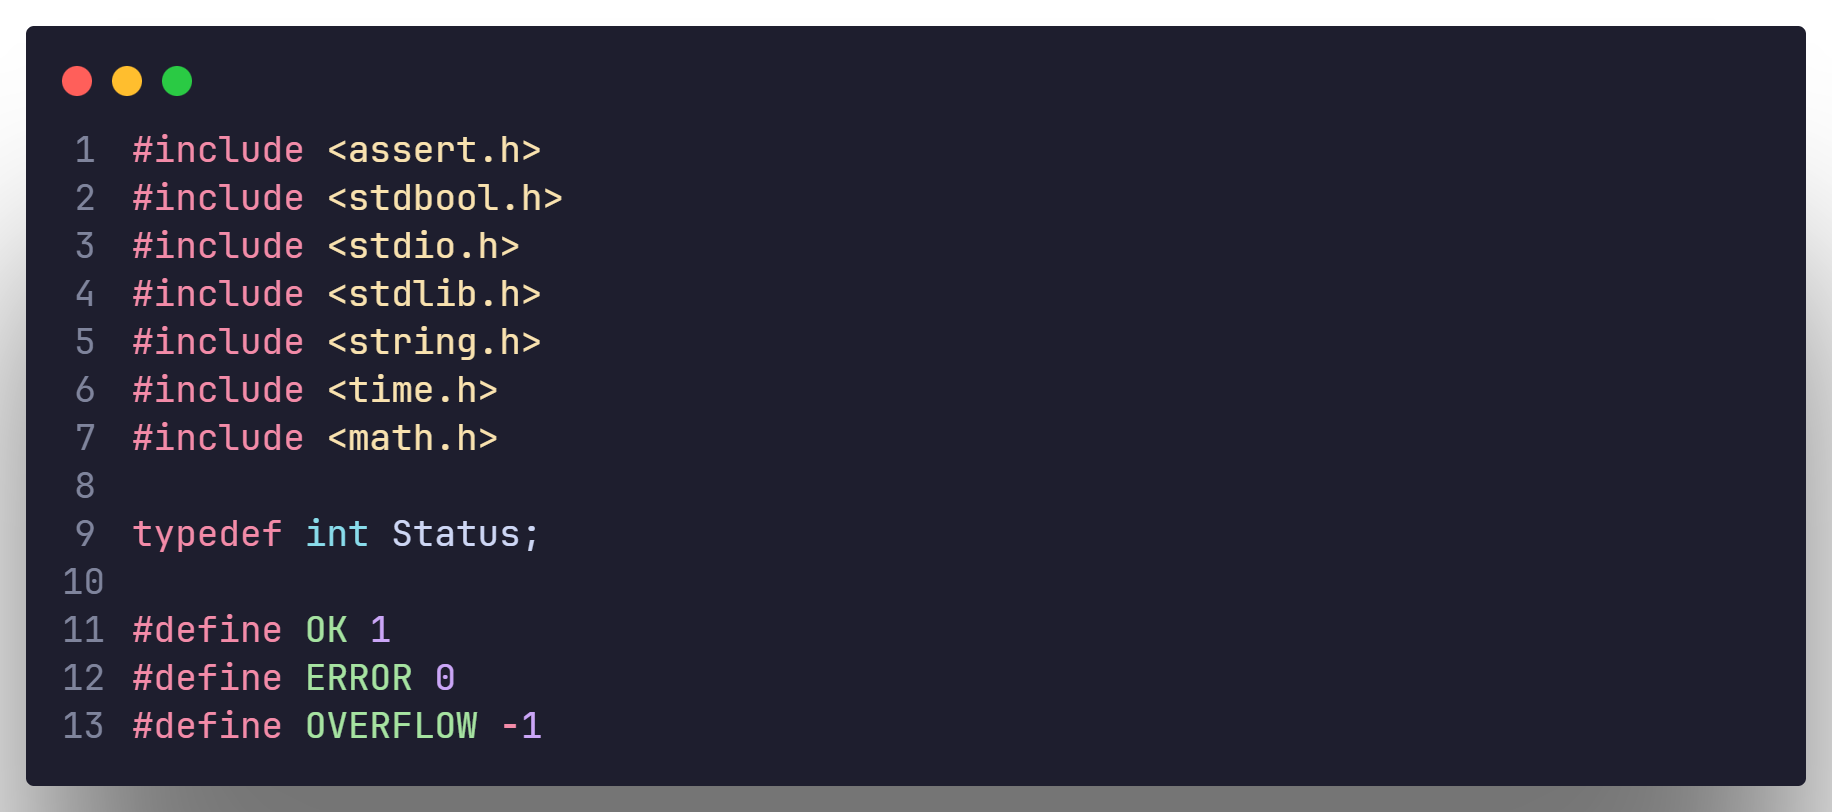
\includegraphics[scale=0.2]{"figure/Note/LinearList/common.png"}
\end{figure} 

\subsubsection{顺序表定义和函数声明}
\begin{figure}[H]
    \centering
    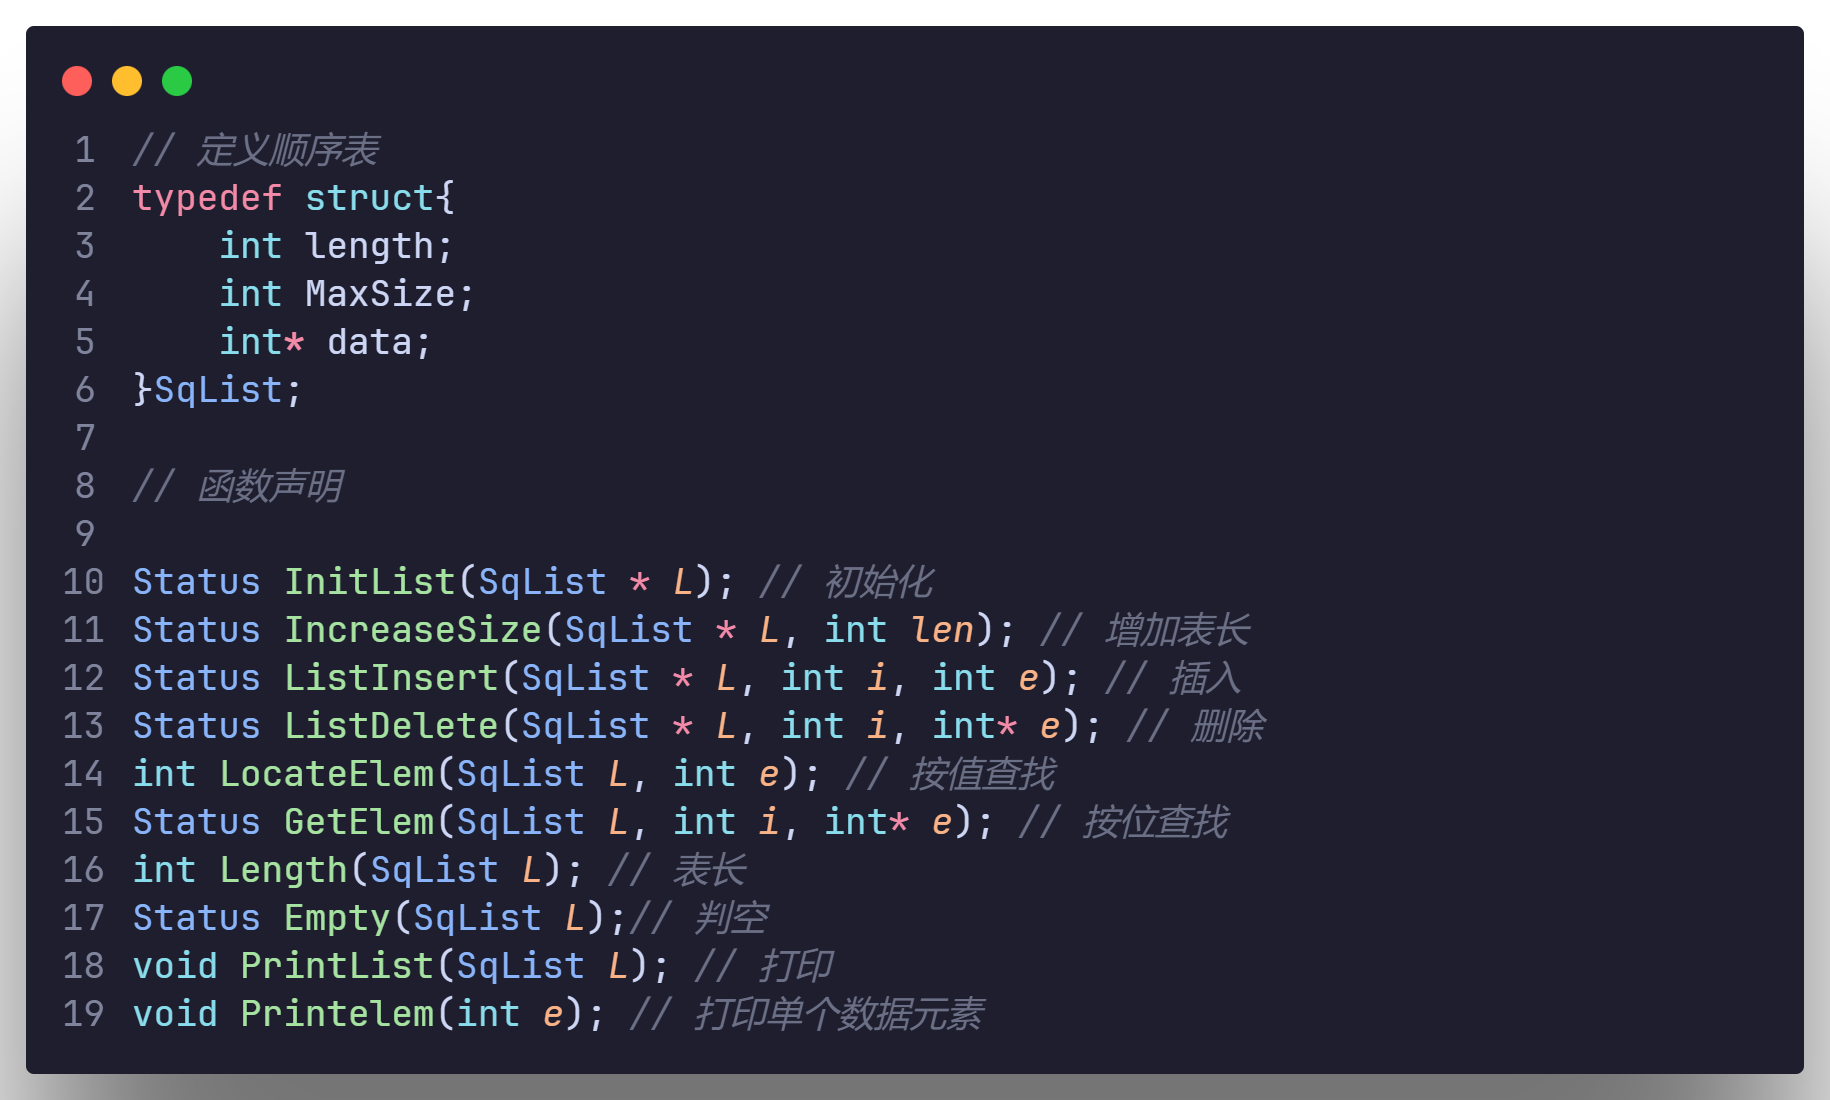
\includegraphics[scale=0.2]{"figure/Note/LinearList/SqFunction.png"}
\end{figure} 

\subsubsection{顺序表初始化}

\begin{figure}[H]
    \centering
    \includegraphics[scale=0.2]{"figure/Note/LinearList/SqInit.png"}
\end{figure} 

\subsubsection{顺序表增加}

\begin{figure}[H]
    \centering
    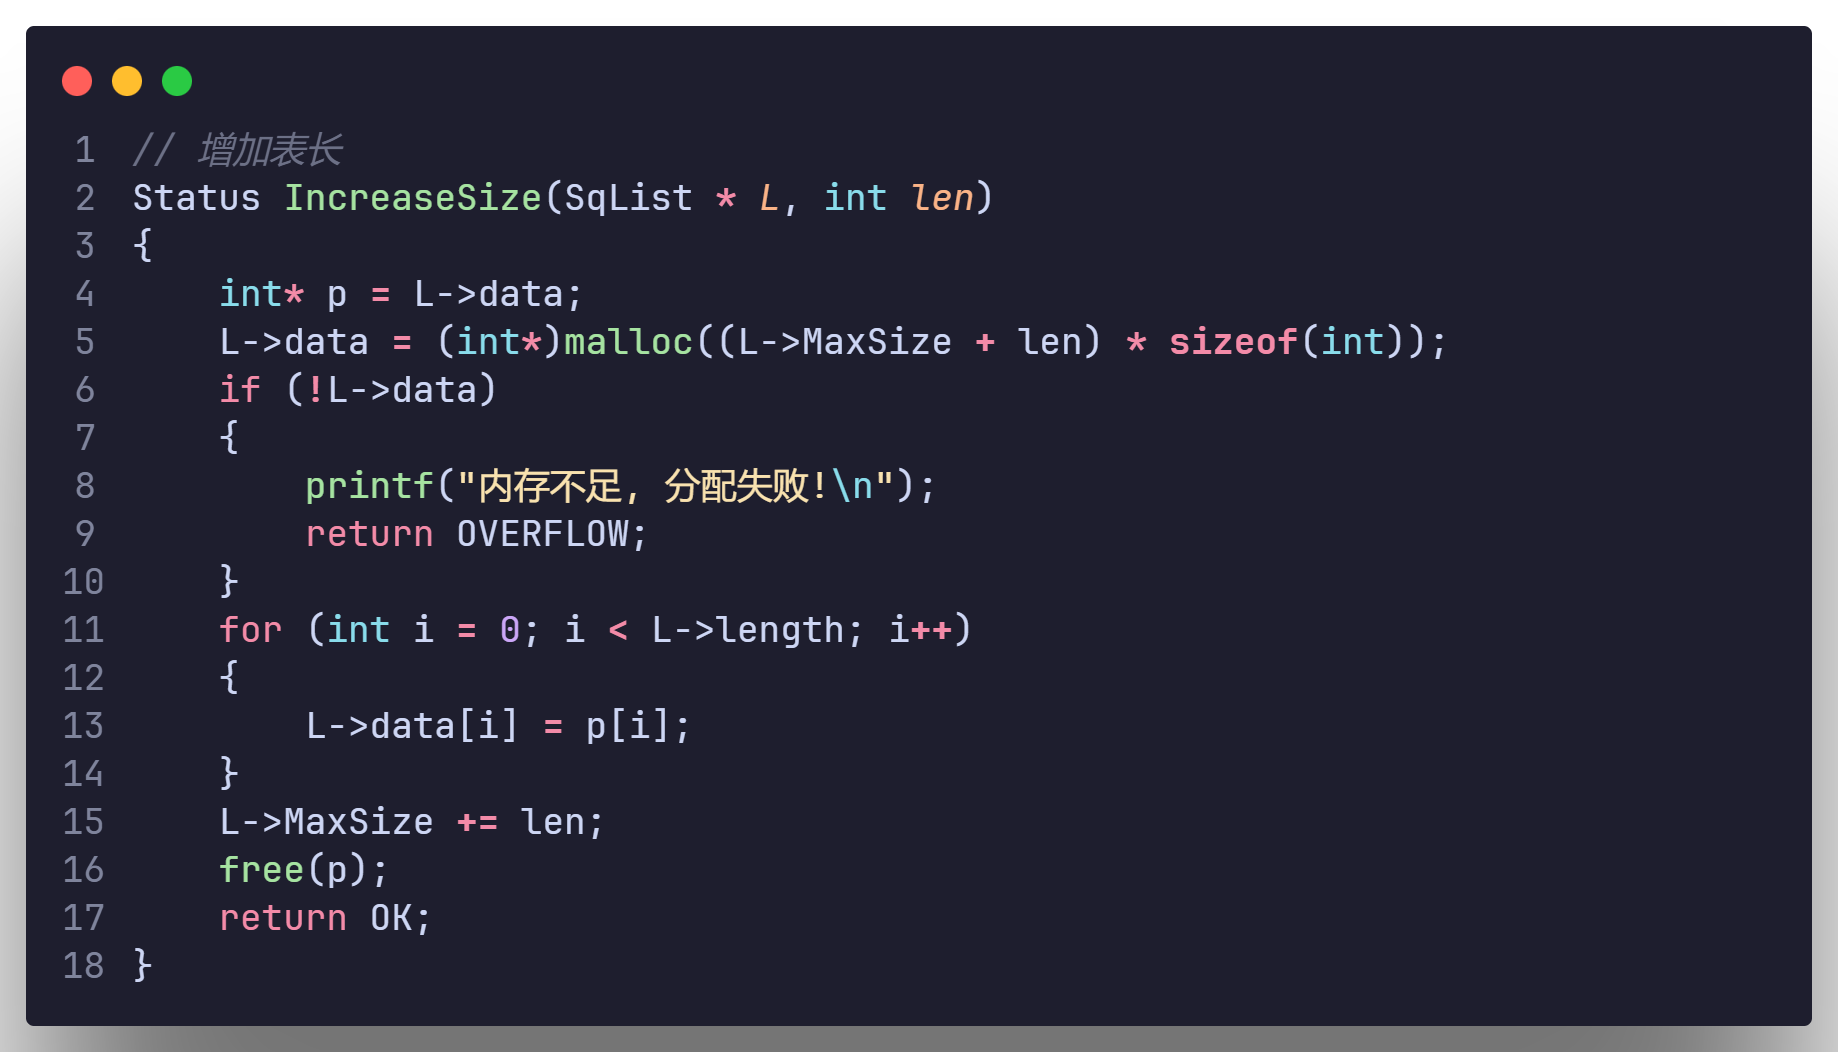
\includegraphics[scale=0.2]{"figure/Note/LinearList/SqIncrease.png"}
\end{figure} 

\subsubsection{顺序表插入}

\begin{figure}[H]
    \centering
    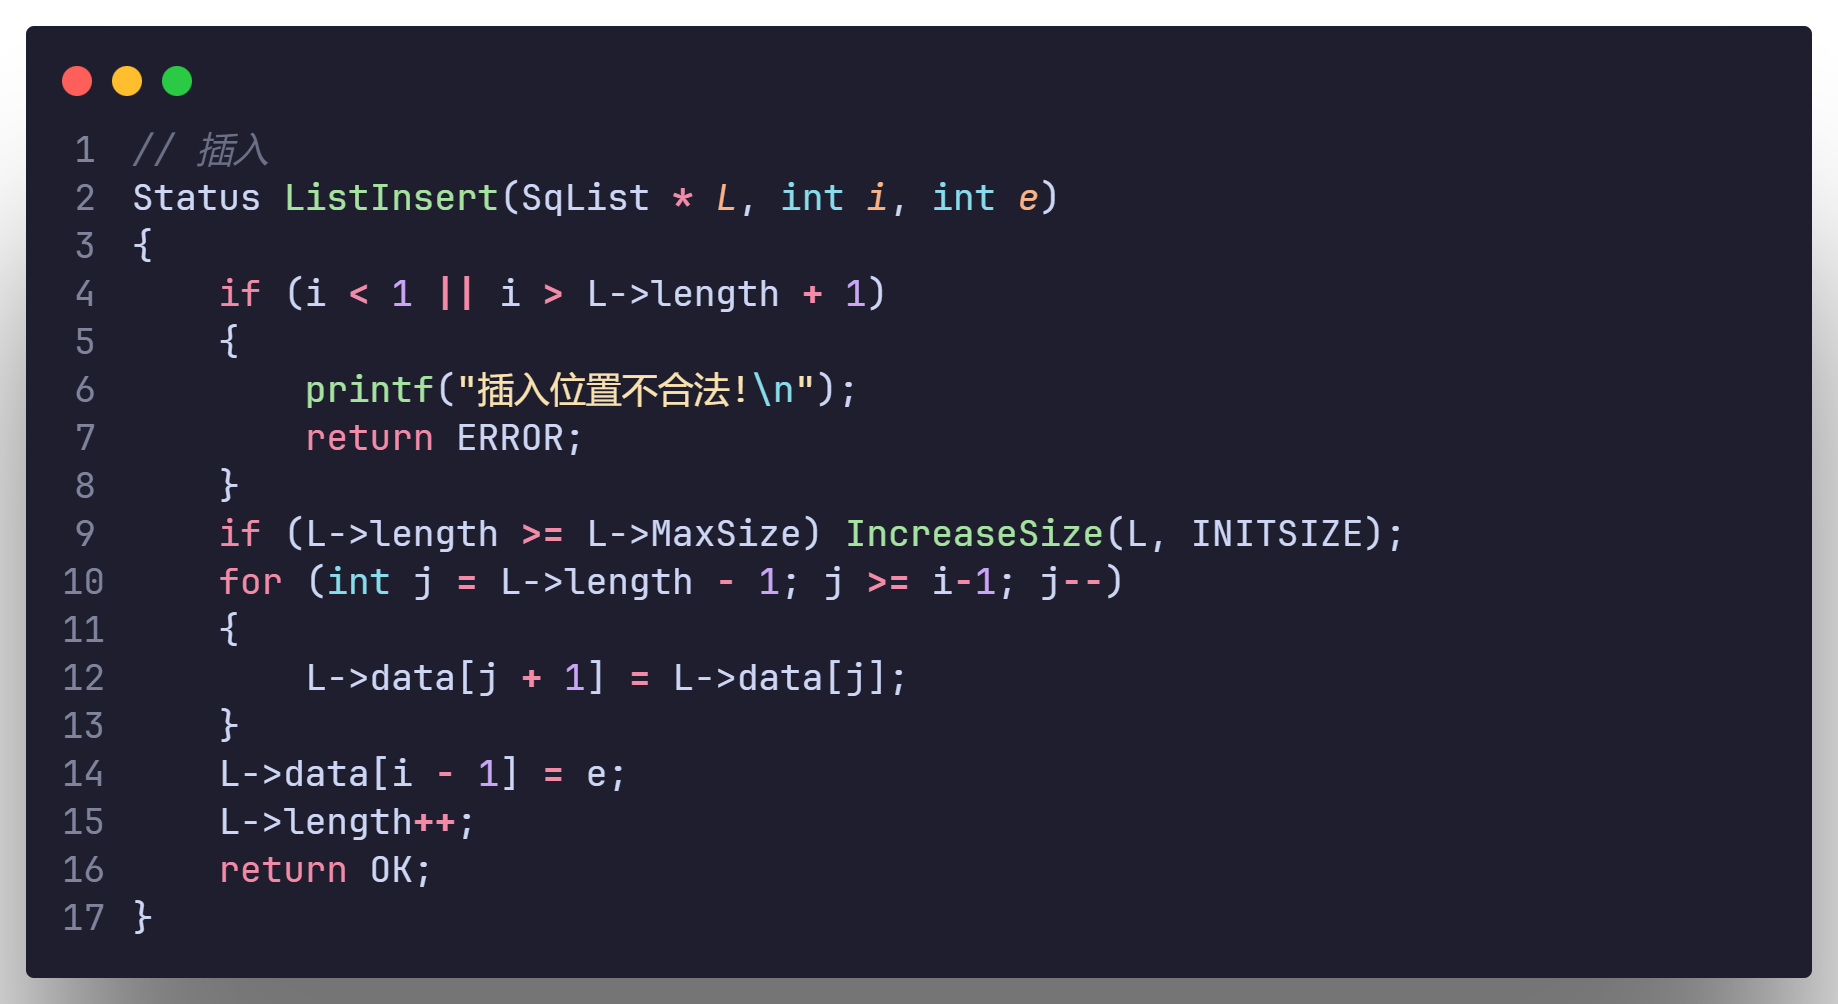
\includegraphics[scale=0.2]{"figure/Note/LinearList/SqInsert.png"}
\end{figure} 

\subsubsection{顺序表删除}

\begin{figure}[H]
    \centering
    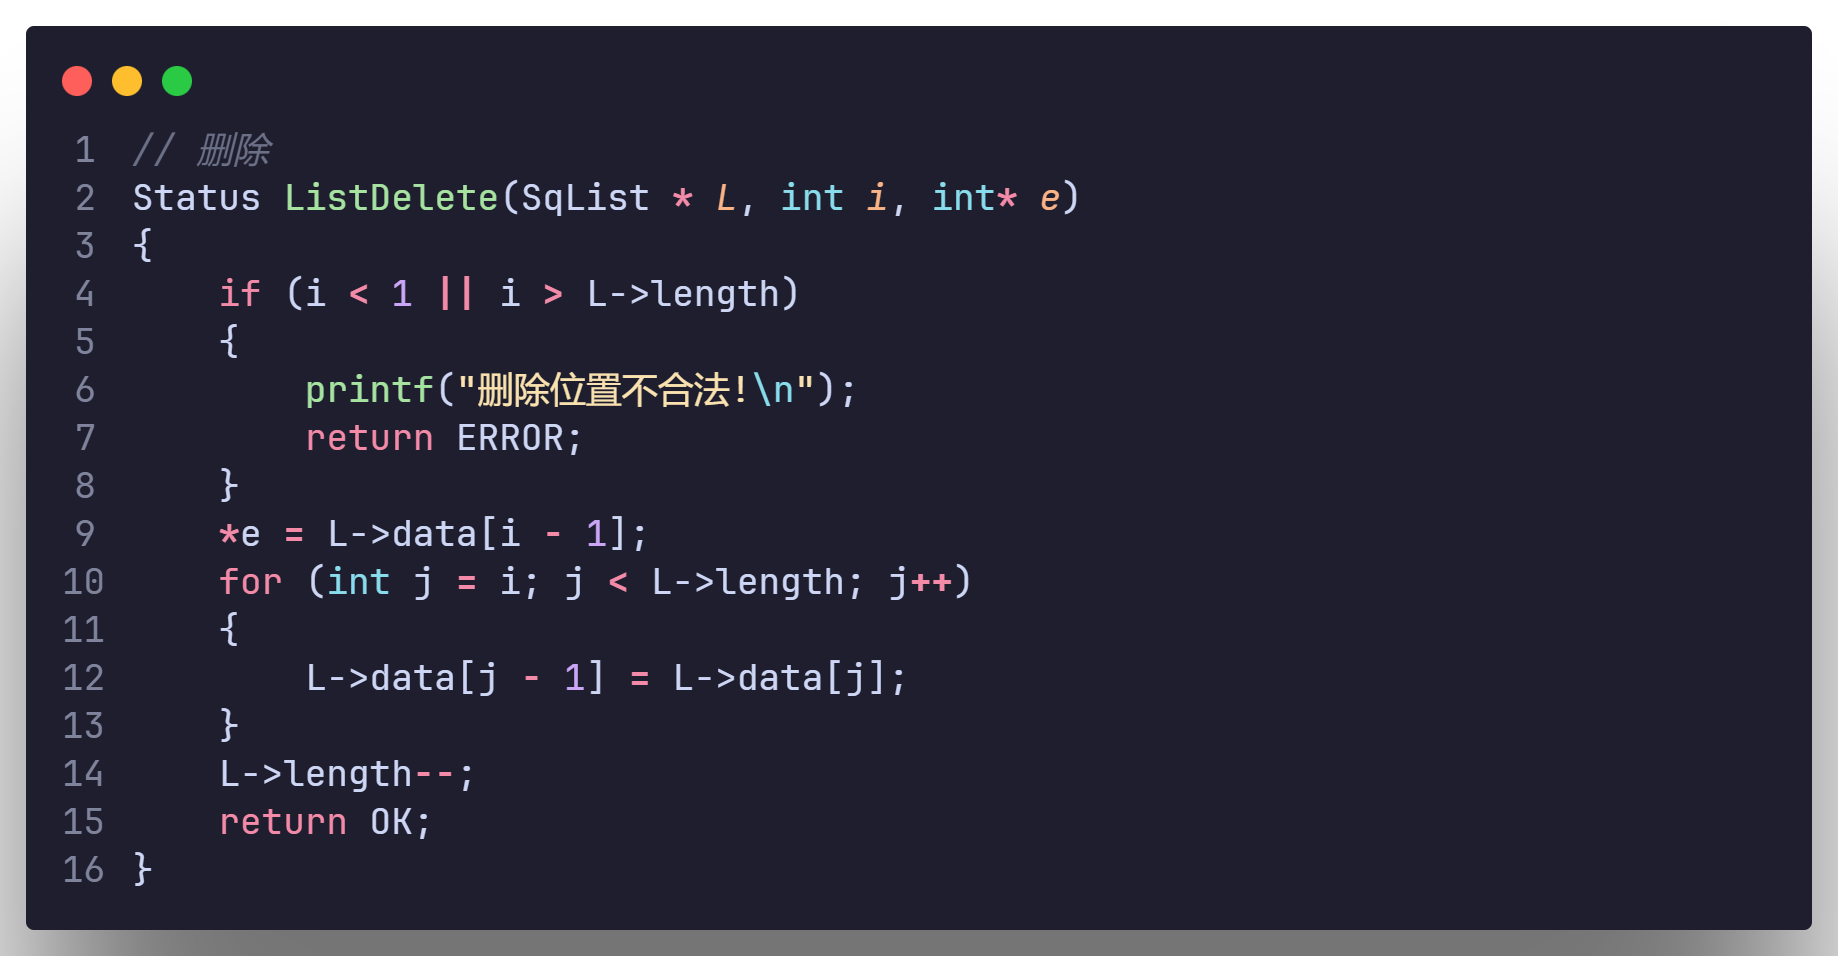
\includegraphics[scale=0.2]{"figure/Note/LinearList/SqDel.png"}
\end{figure} 

\subsubsection{顺序表查找}

(1). 按位置查找

\begin{figure}[H]
    \centering
    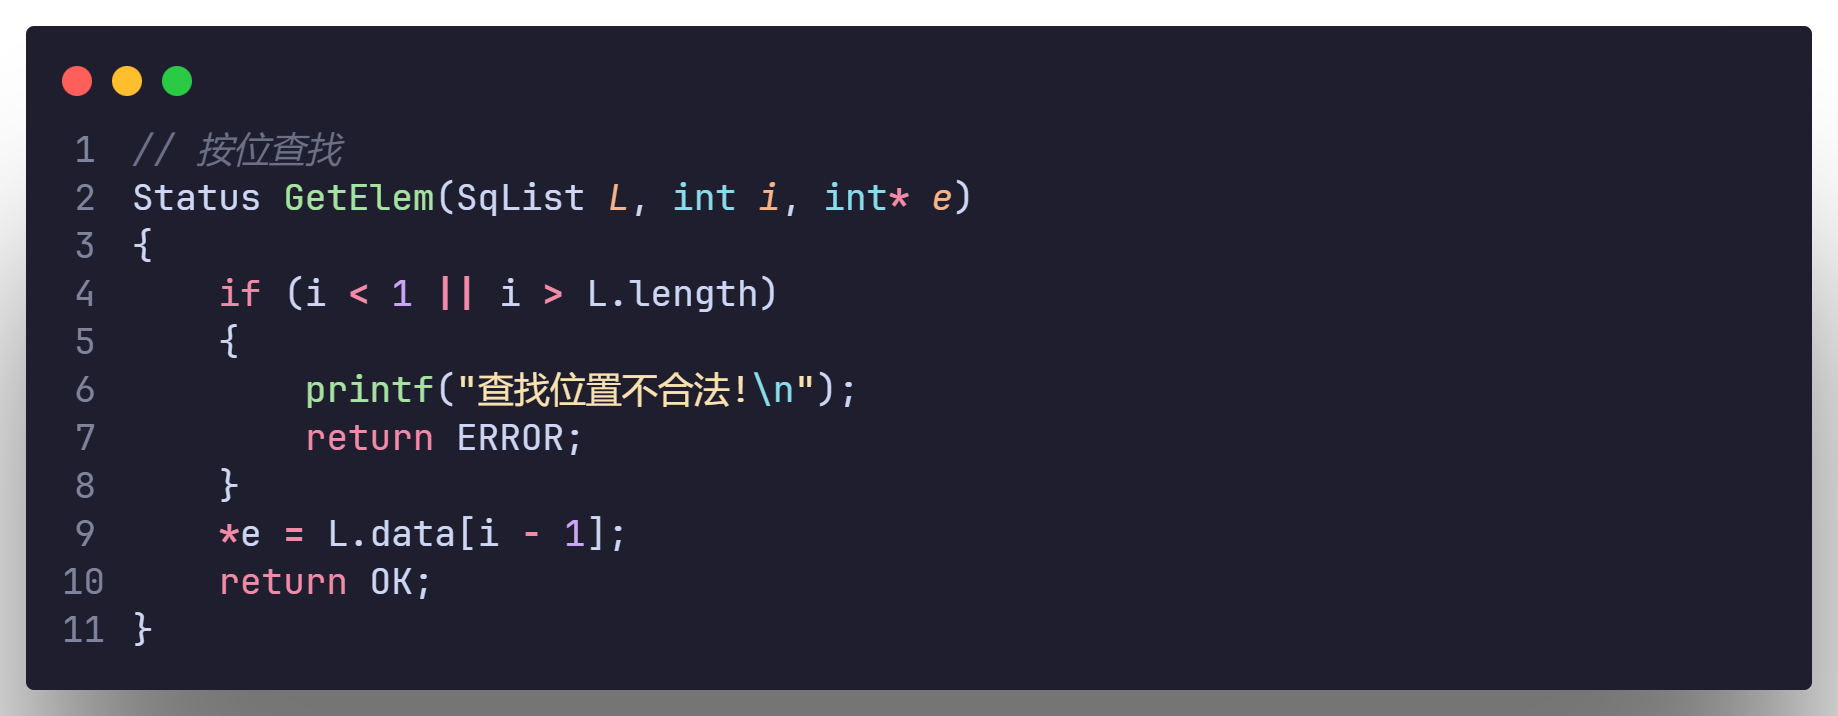
\includegraphics[scale=0.2]{"figure/Note/LinearList/SqNumSer.png"}
\end{figure} 

(2). 按值查找

\begin{figure}[H]
    \centering
    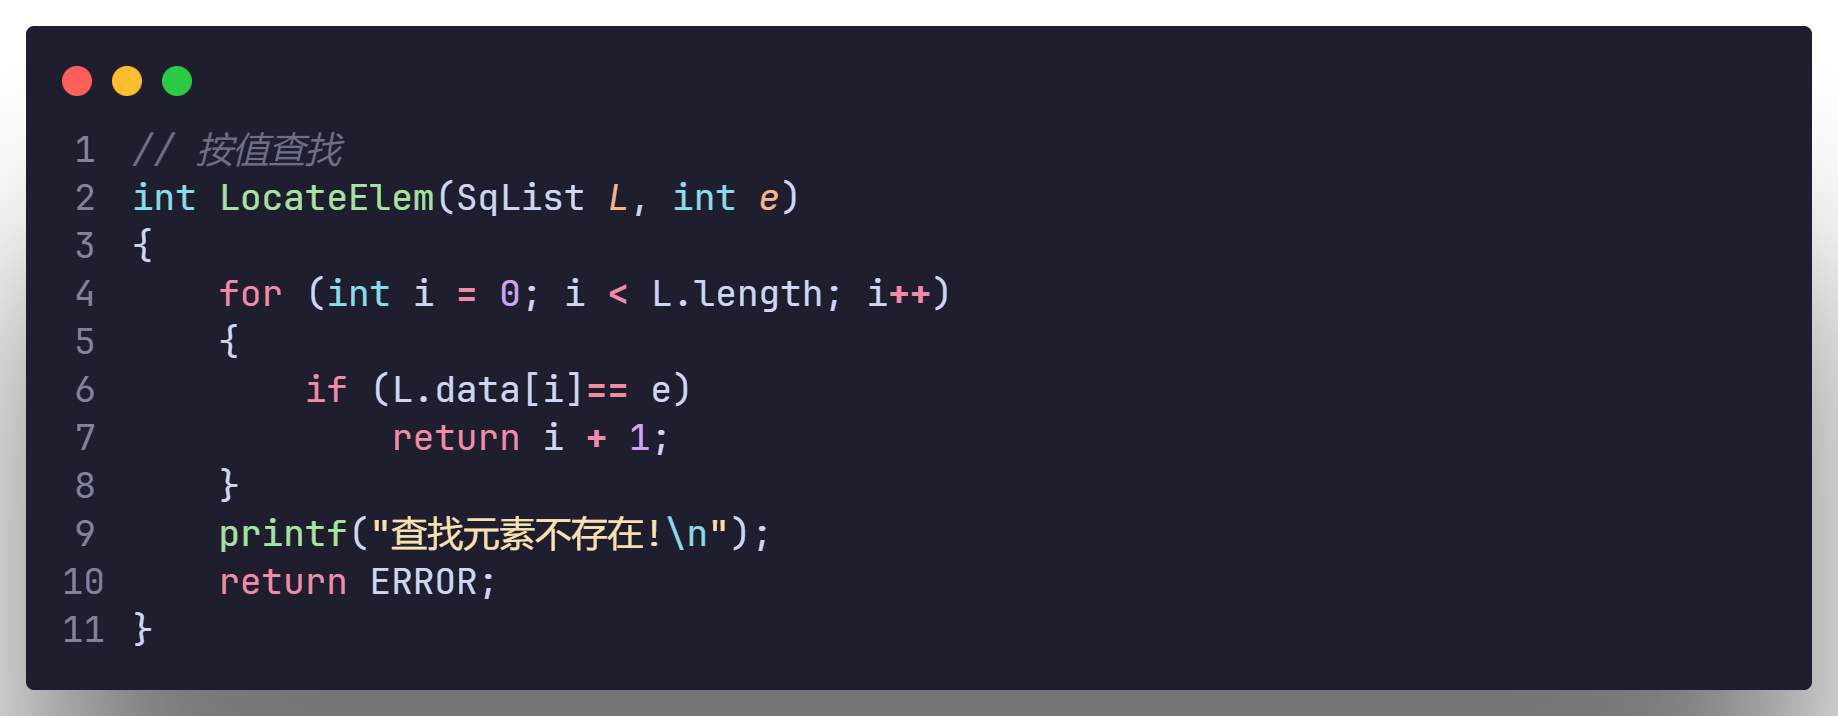
\includegraphics[scale=0.2]{"figure/Note/LinearList/SqItemSer.png"}
\end{figure} 


\subsubsection{顺序表辅助函数}

(1). $Length$ 

\begin{figure}[H]
    \centering
    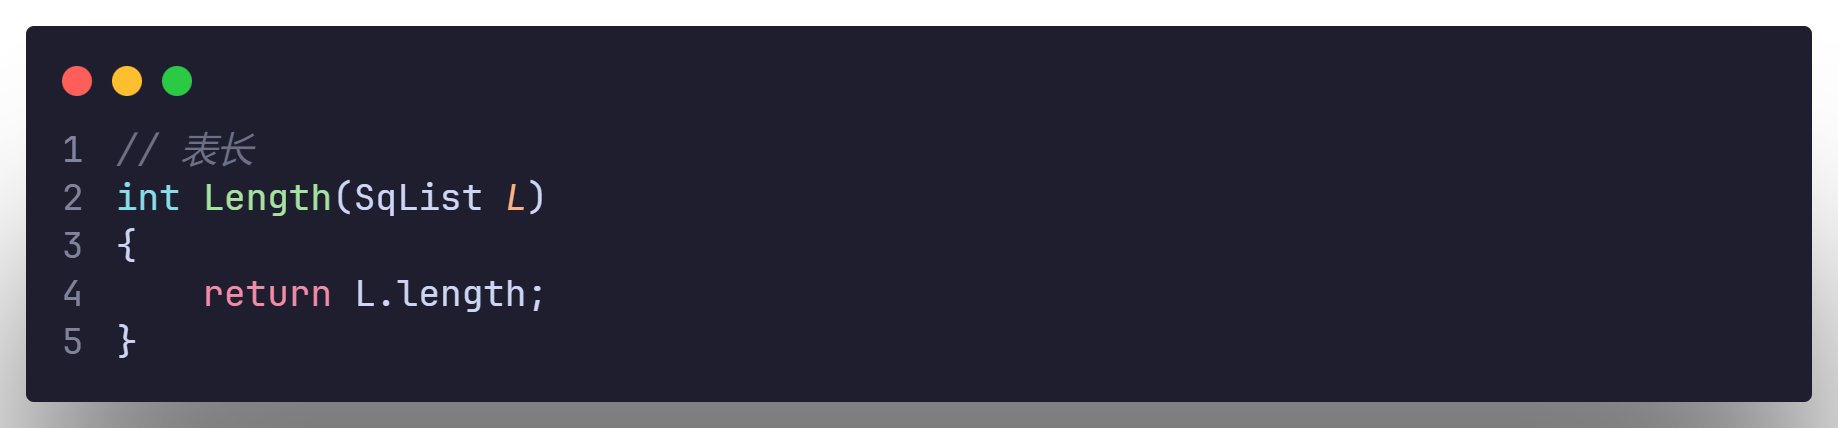
\includegraphics[scale=0.2]{"figure/Note/LinearList/SqLen.png"}
\end{figure} 

(2). $Empty$ 

\begin{figure}[H]
    \centering
    \includegraphics[scale=0.2]{"figure/Note/LinearList/SqEmpty.png"}
\end{figure} 

(3). $PrintList$

\begin{figure}[H]
    \centering
    \includegraphics[scale=0.2]{"figure/Note/LinearList/SqPrint.png"}
\end{figure} 

\section{线性表的链式表示}
\subsection{单链表}
\begin{definition}[单链表]
    \begin{enumerate}
        \item 单链表第一个元素在删除和增加需要特殊处理
        \item 头插法和尾插法的区别, 头插法实现反置
        \item 在增删、初始化操作传入引用, 在判空、打印以及求表长传入值
    \end{enumerate}
\end{definition}
\subsubsection{单链表定义和函数声明}

\begin{figure}[H]
    \centering
    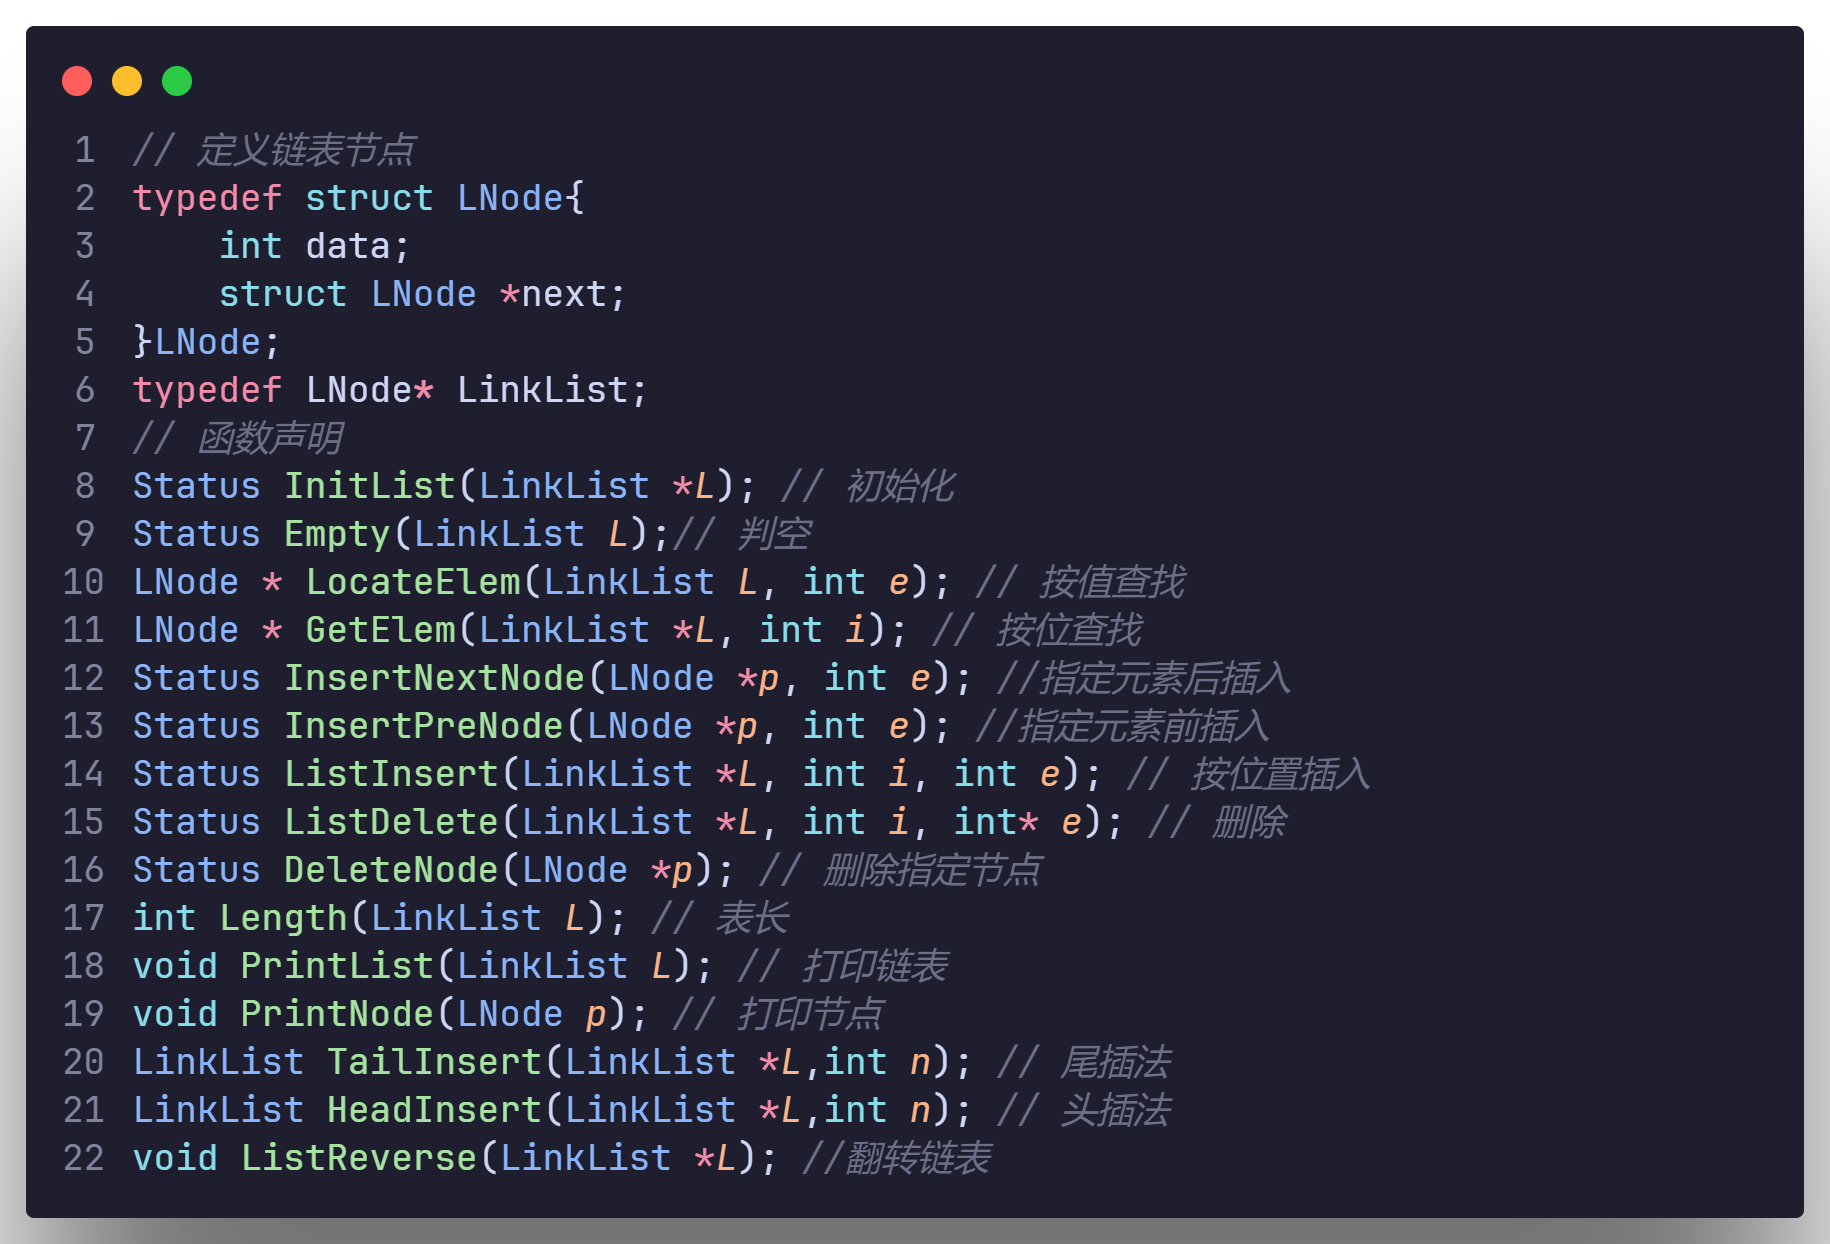
\includegraphics[scale=0.2]{"figure/Note/LinearList/SlFunction.png"}
\end{figure} 

\subsubsection{单链表初始化}

\begin{figure}[H]
    \centering
    \includegraphics[scale=0.2]{"figure/Note/LinearList/SlInit.png"}
\end{figure} 

\subsubsection{单链表查找}

(1). 按位置查找
\begin{figure}[H]
    \centering
    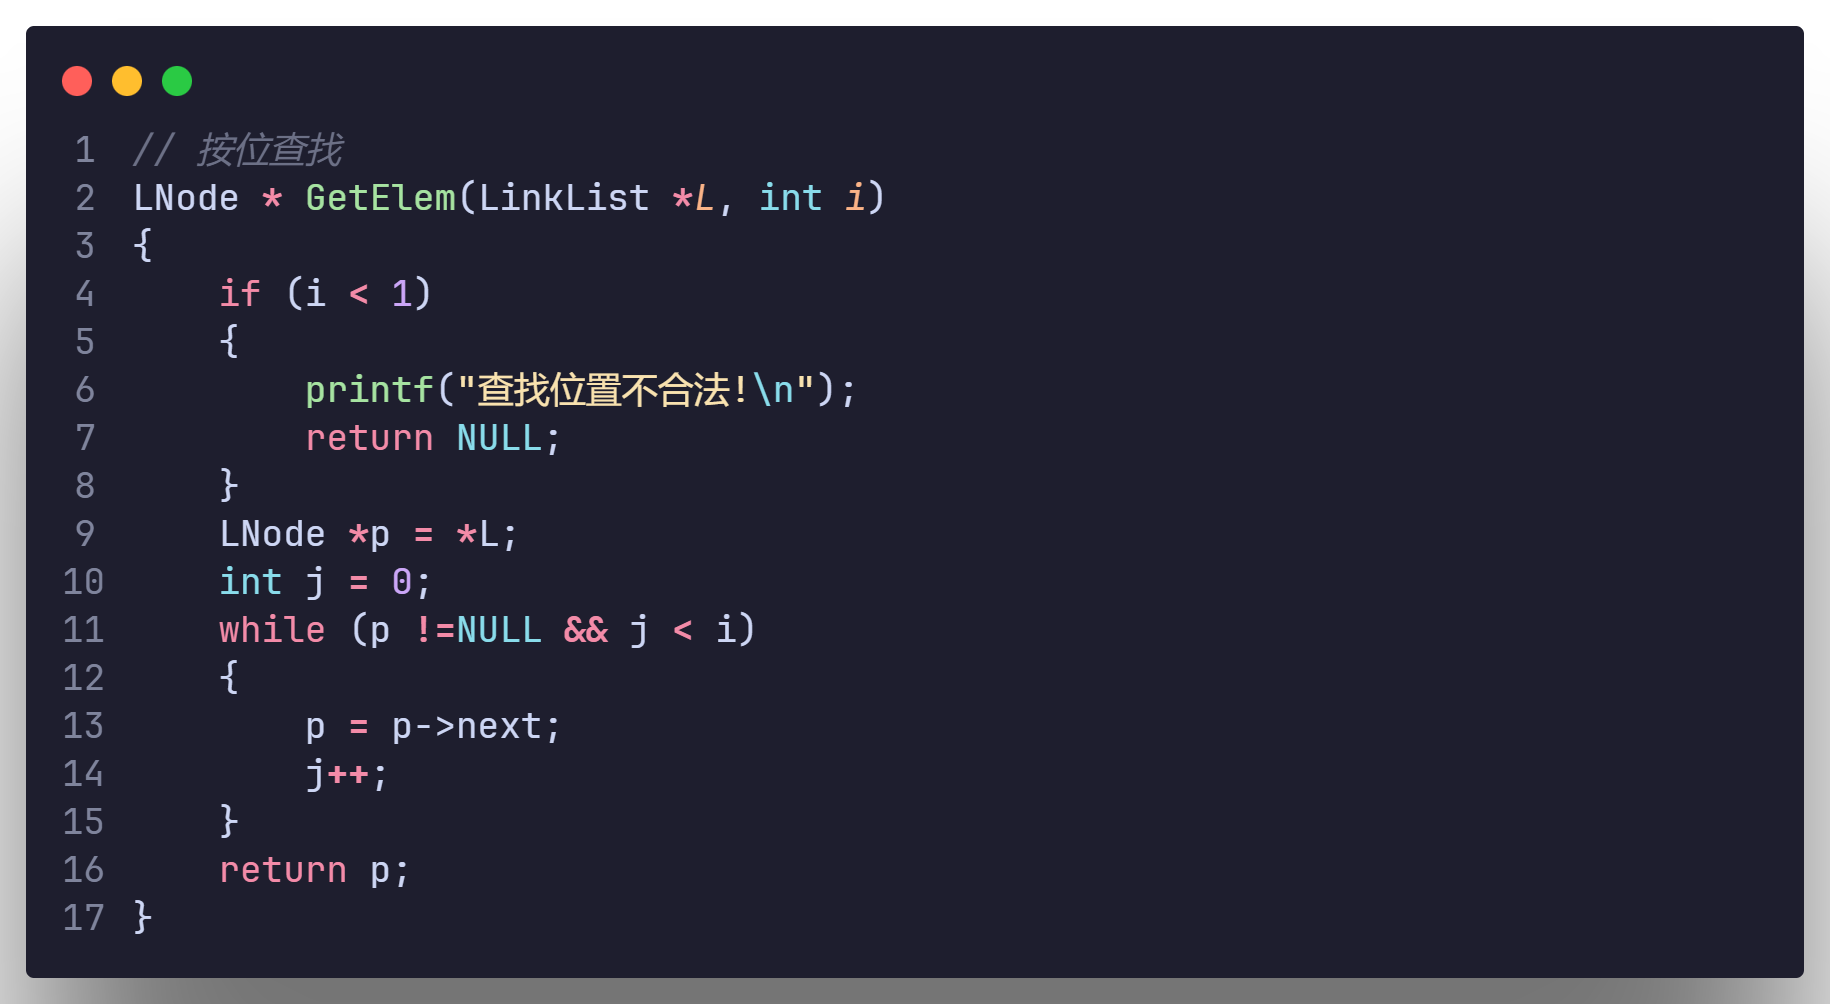
\includegraphics[scale=0.2]{"figure/Note/LinearList/SlNumSer.png"}
\end{figure} 

(2). 按值查找

\begin{figure}[H]
    \centering
    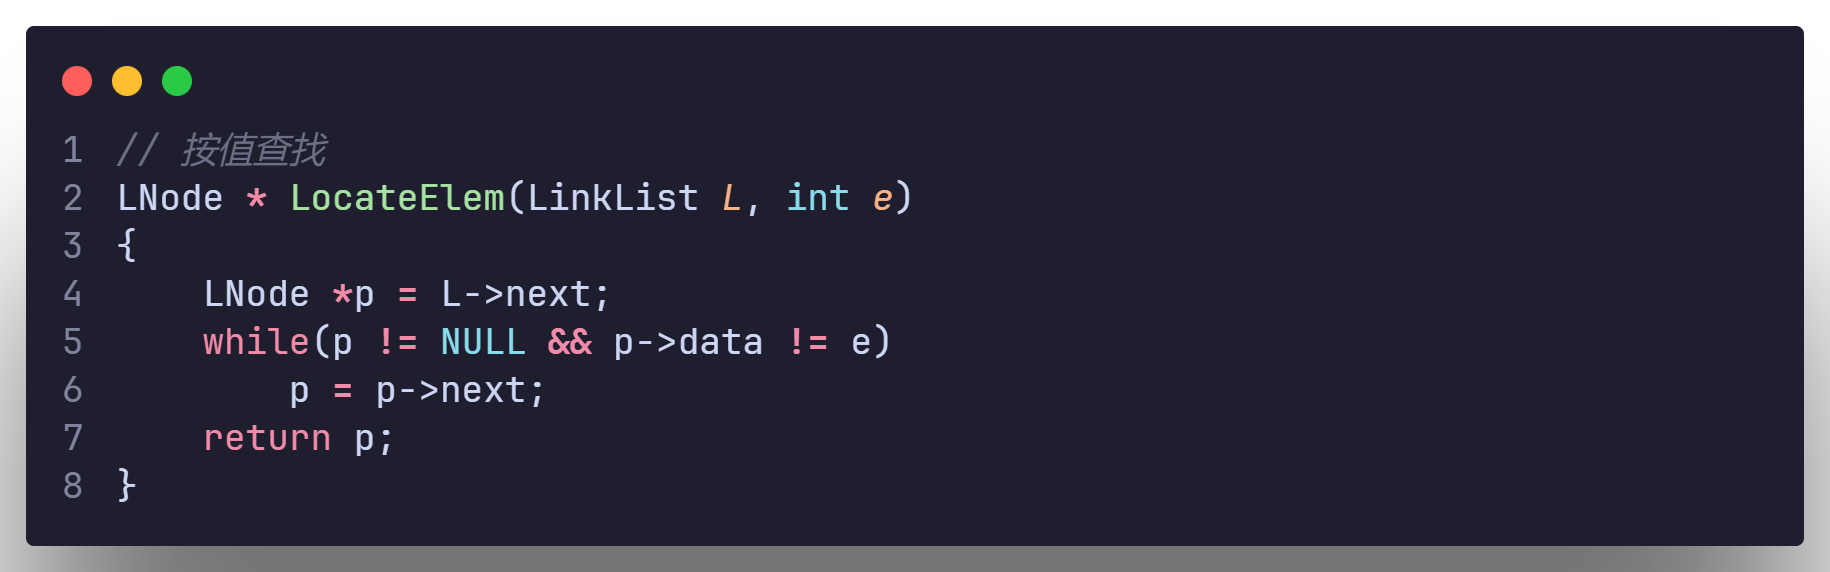
\includegraphics[scale=0.2]{"figure/Note/LinearList/SlItemSer.png"}
\end{figure} 

\subsubsection{单链表插入}

(1). 指定元素后插入

\begin{figure}[H]
    \centering
    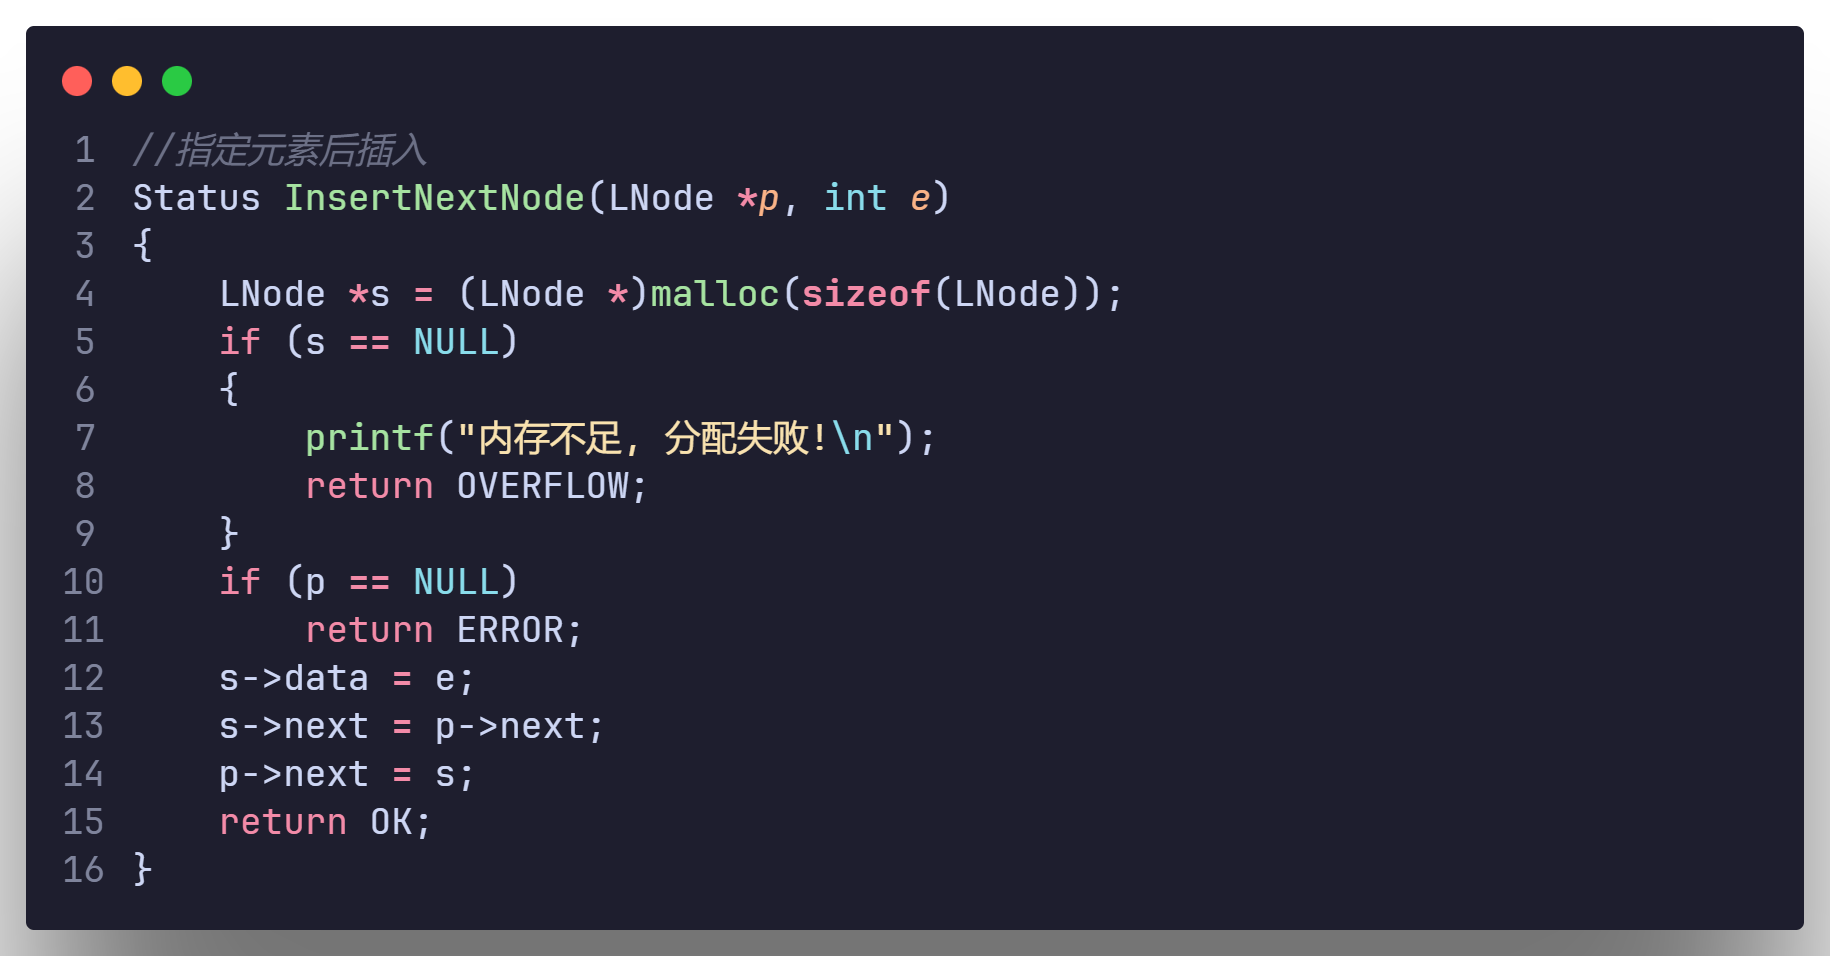
\includegraphics[scale=0.2]{"figure/Note/LinearList/SlBInsert.png"}
\end{figure}

(2). 指定元素前插入

\begin{figure}[H]
    \centering
    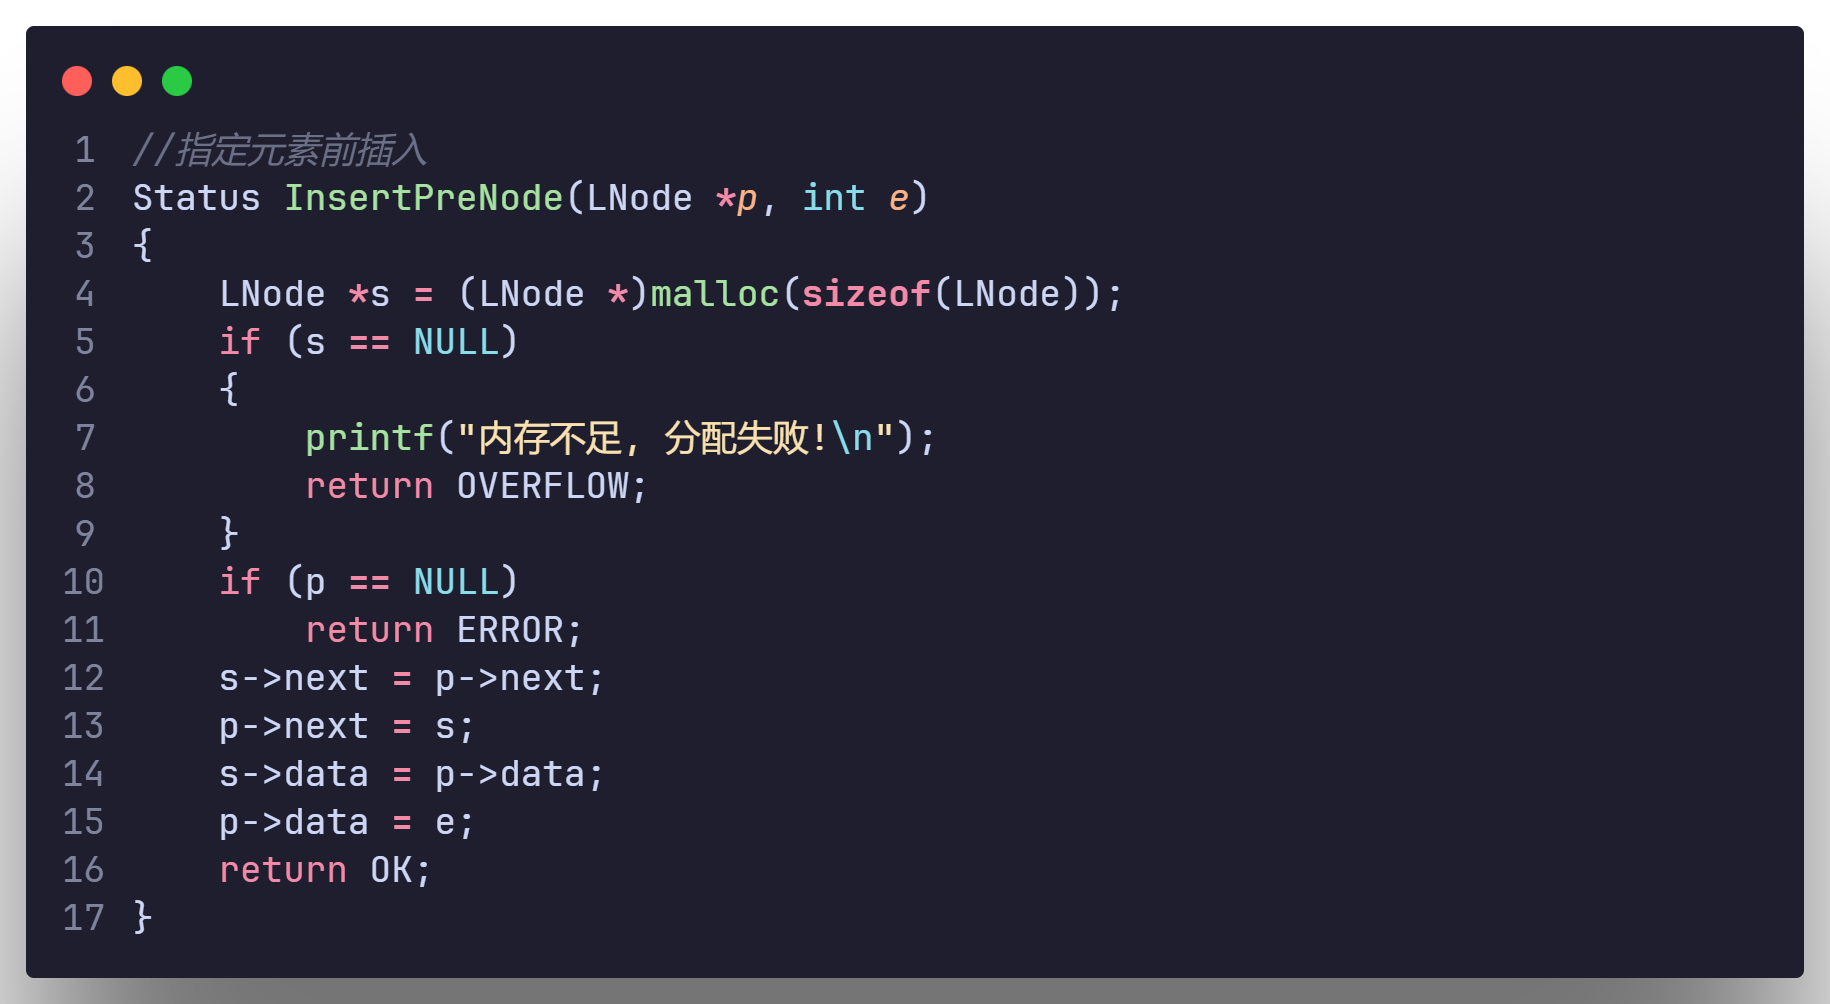
\includegraphics[scale=0.2]{"figure/Note/LinearList/SlFInsert.png"}
\end{figure}

(3). 按位置插入

\begin{figure}[H]
    \centering
    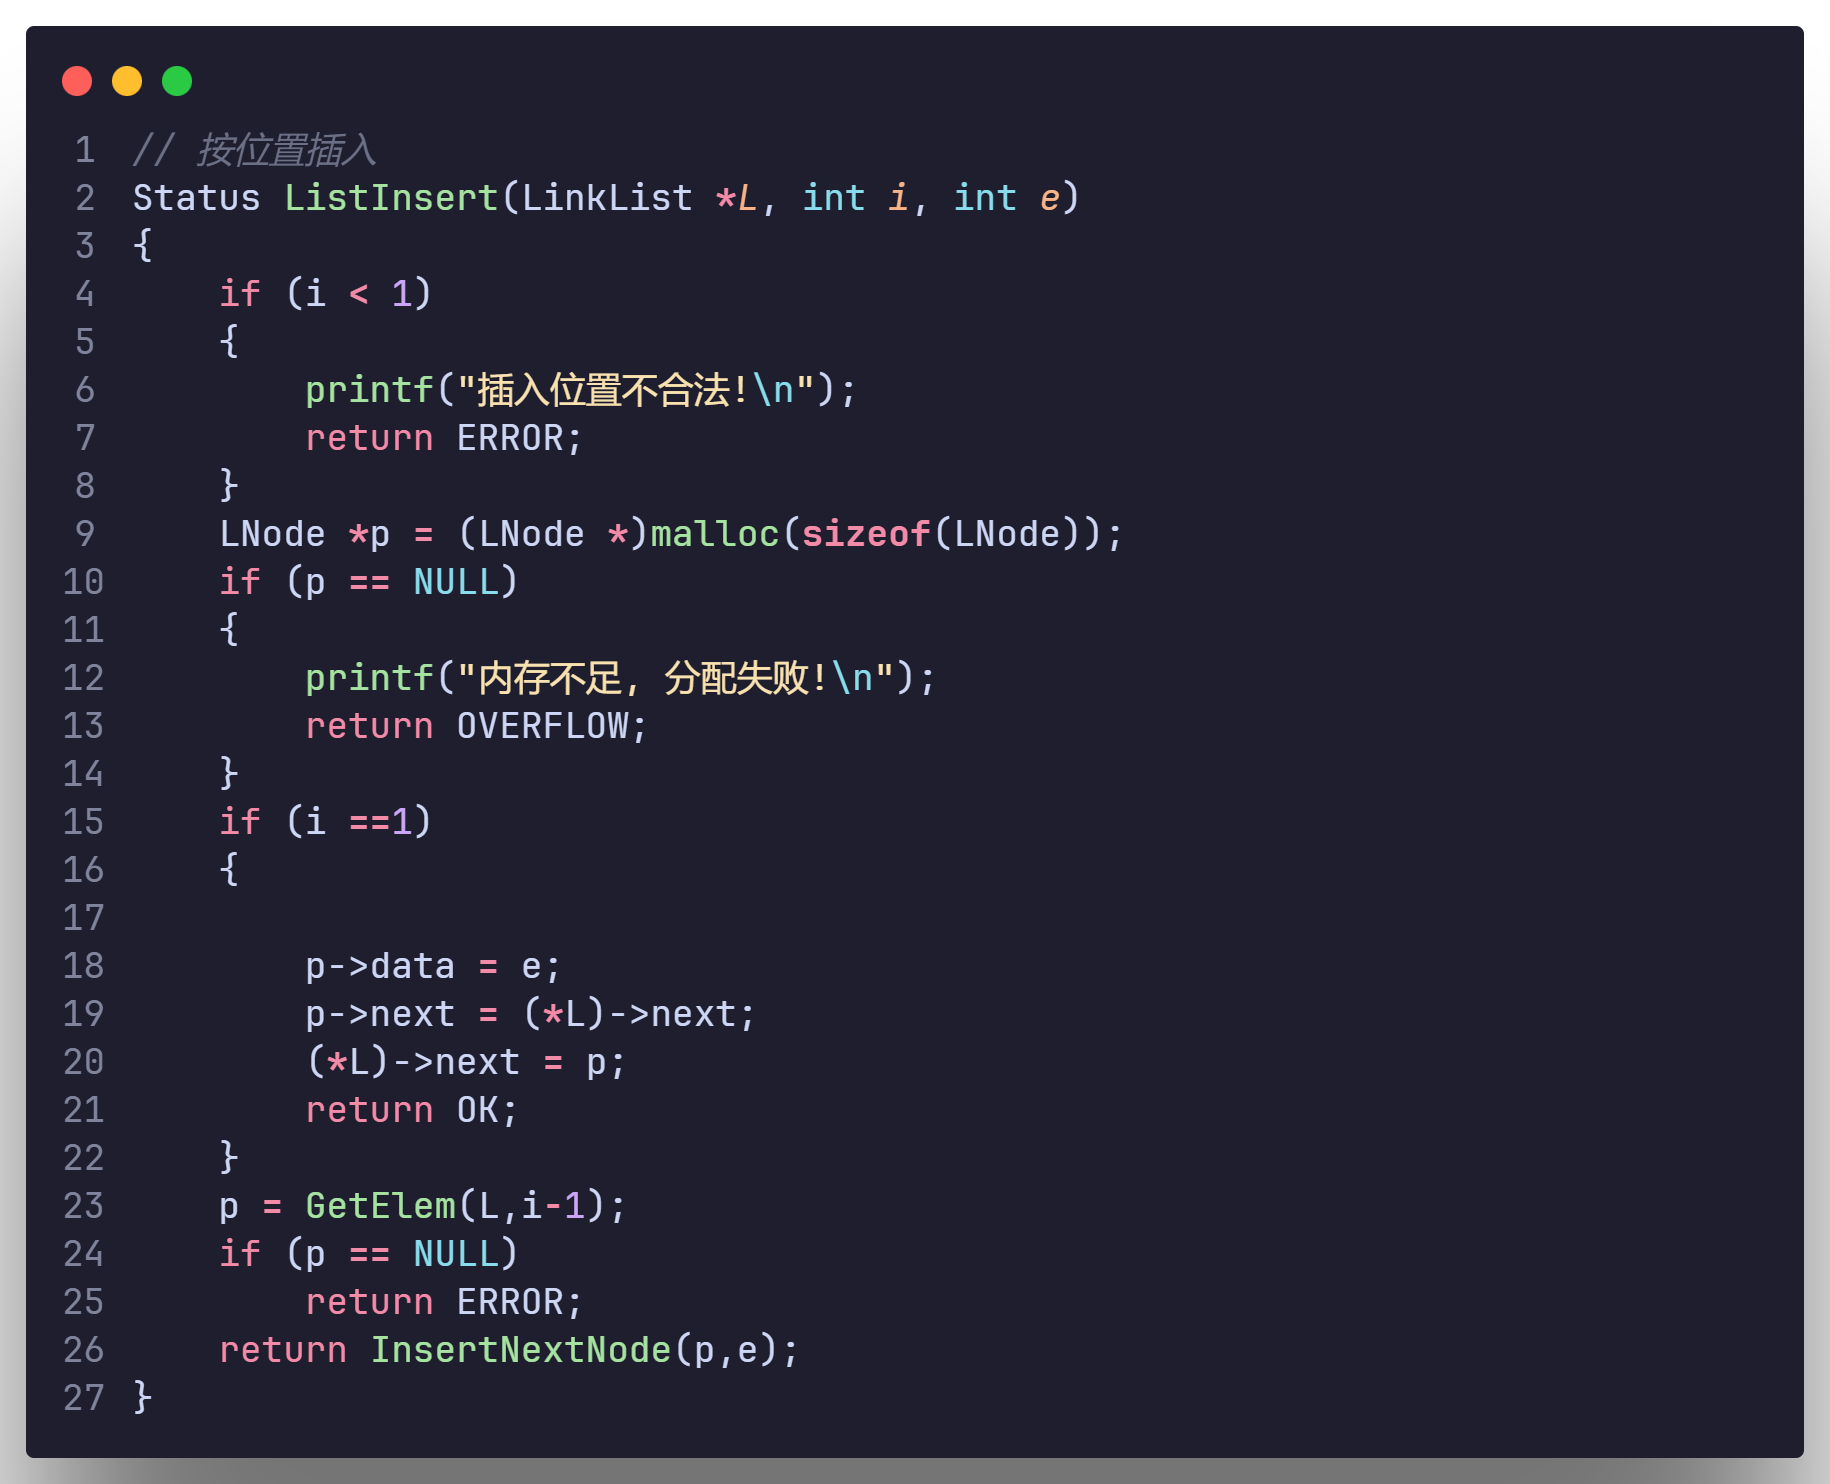
\includegraphics[scale=0.2]{"figure/Note/LinearList/SlInsert.png"}
\end{figure}

\subsubsection{单链表删除}

\begin{figure}[H]
    \centering
    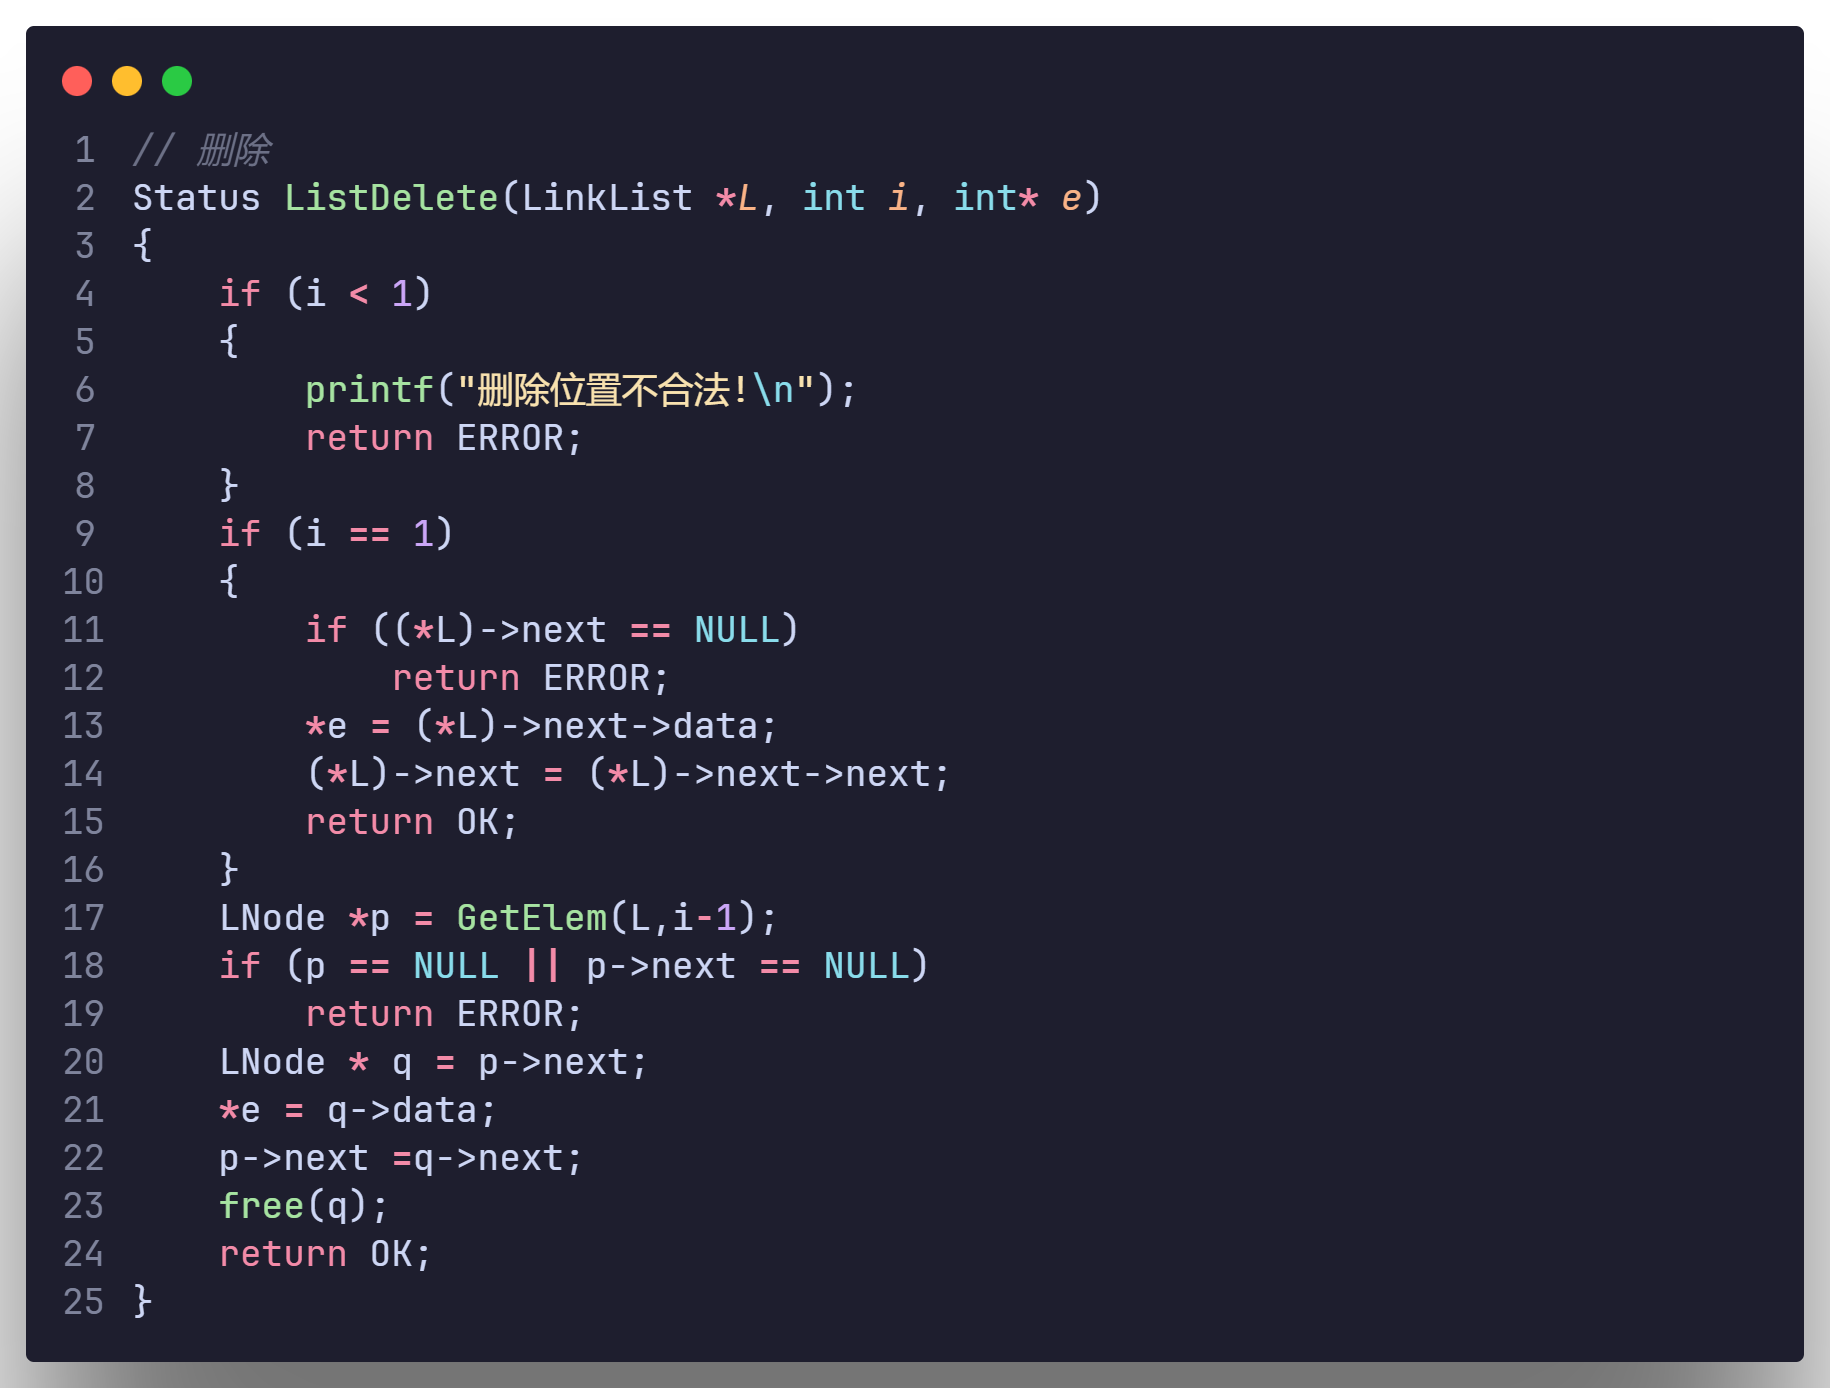
\includegraphics[scale=0.2]{"figure/Note/LinearList/SlDel.png"}
\end{figure}

\subsubsection{单链表辅助函数}

(1). $Length$

\begin{figure}[H]
    \centering
    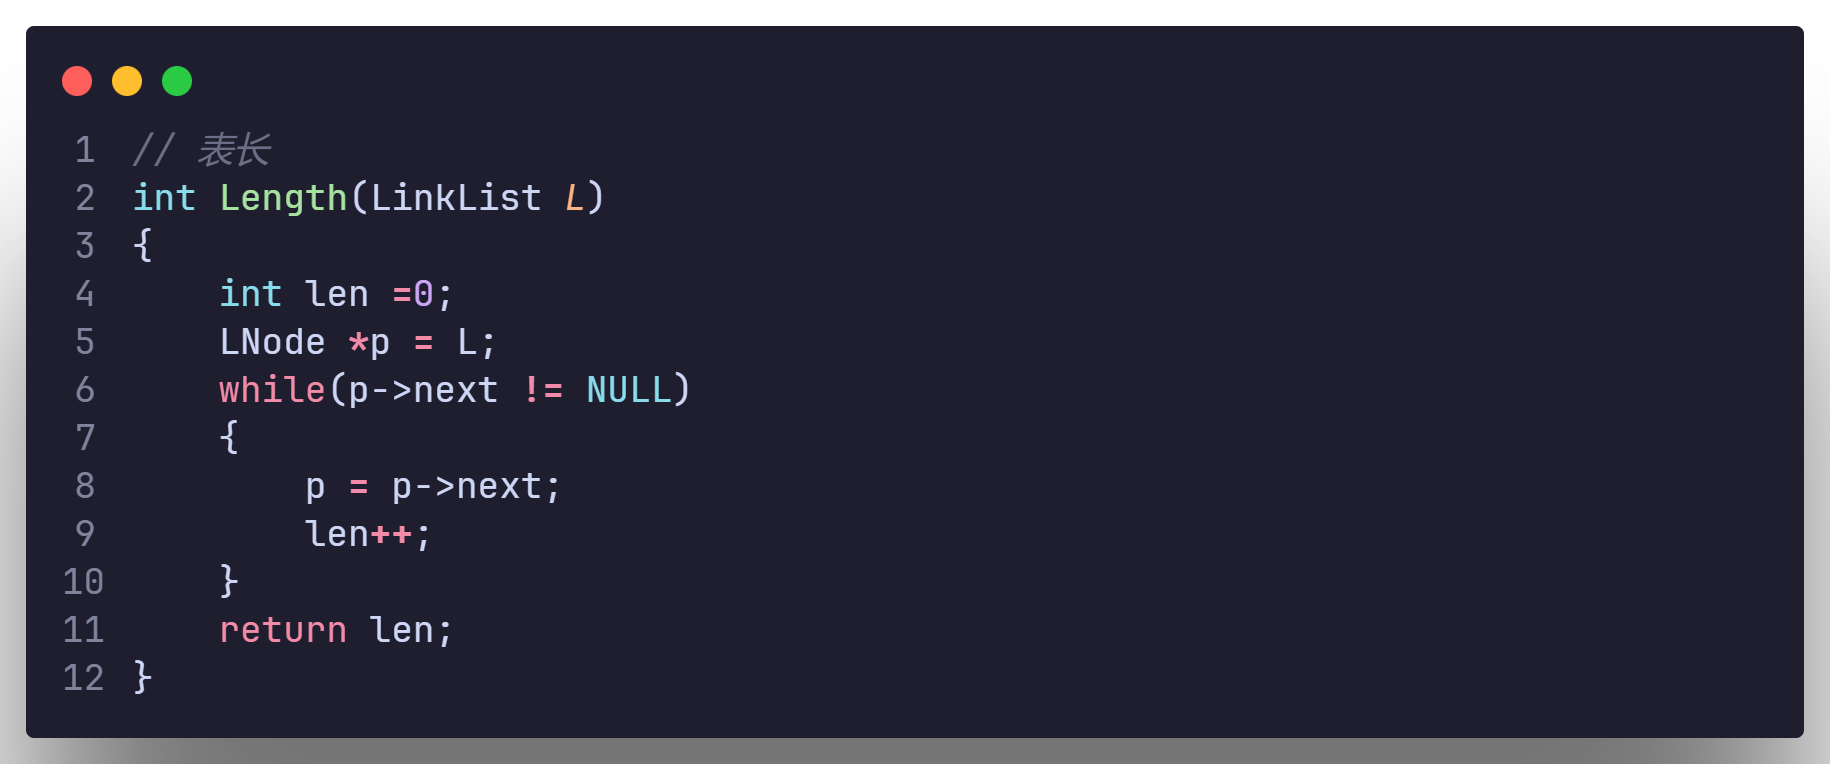
\includegraphics[scale=0.2]{"figure/Note/LinearList/SlLen.png"}
\end{figure}

(2). $Empty$

\begin{figure}[H]
    \centering
    \includegraphics[scale=0.2]{"figure/Note/LinearList/SlEmpty.png"}
\end{figure}

(3). $PrintList$

\begin{figure}[H]
    \centering
    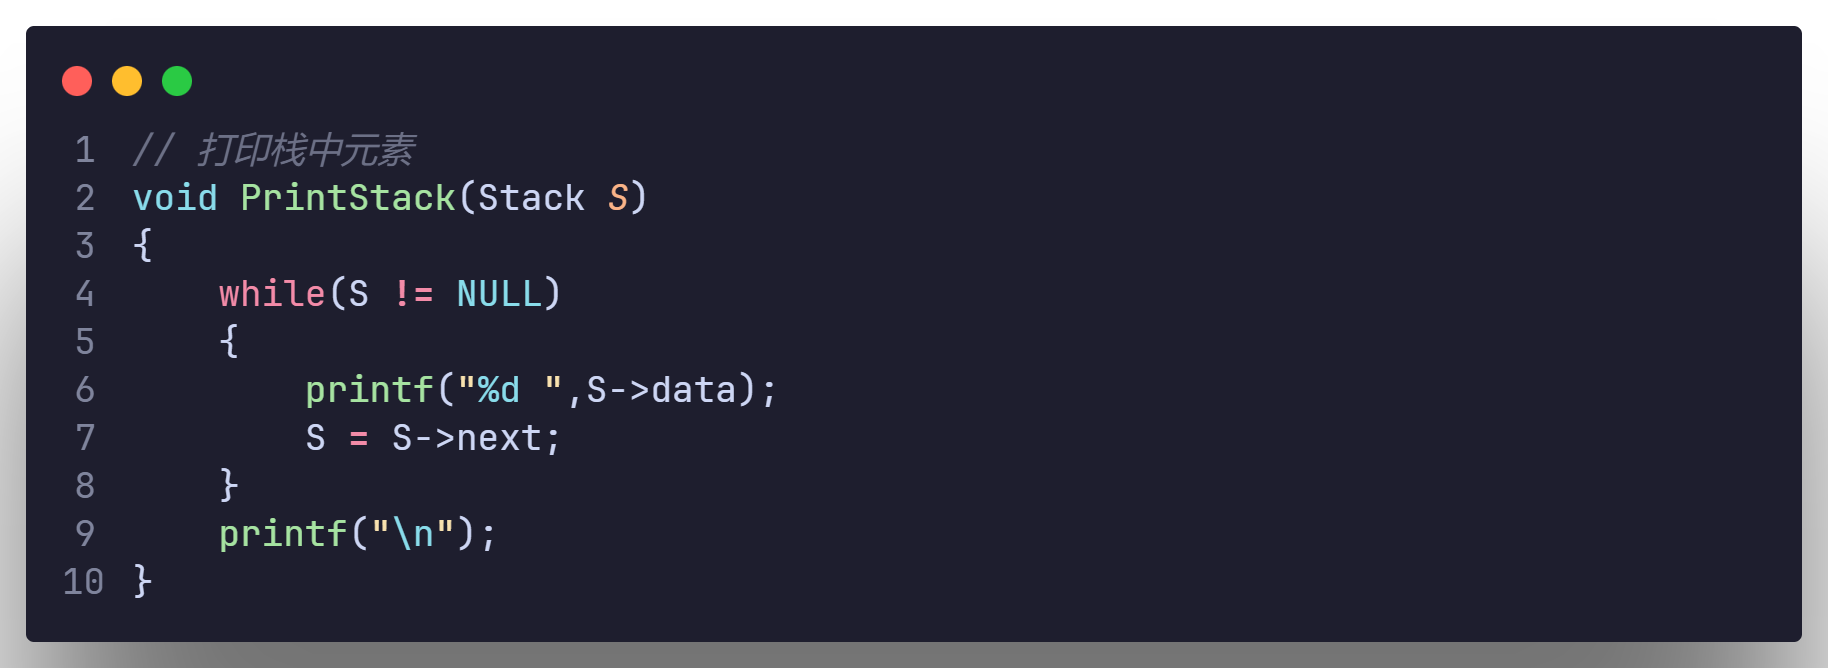
\includegraphics[scale=0.2]{"figure/Note/LinearList/SlPrint.png"}
\end{figure}


\subsubsection{头插法 \& 尾插法}

(1). 头插法

\begin{figure}[H]
    \centering
    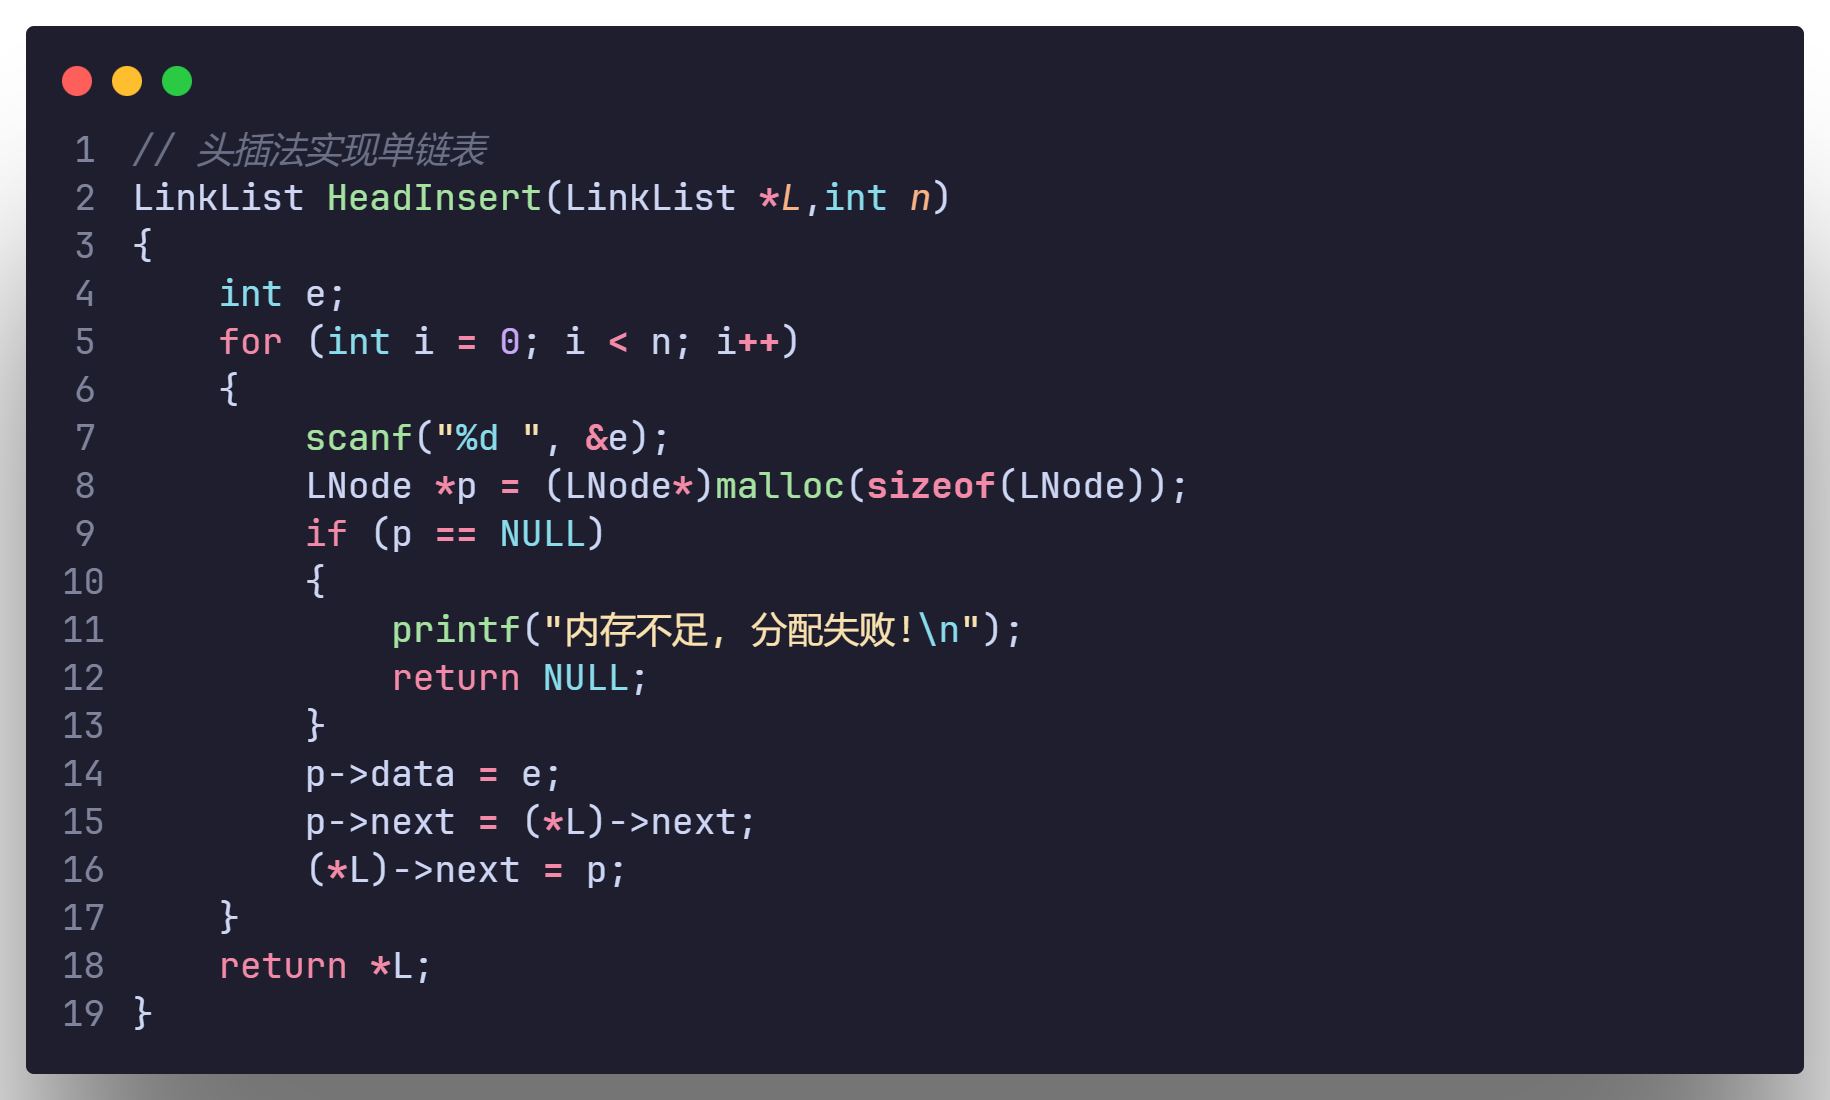
\includegraphics[scale=0.2]{"figure/Note/LinearList/SlHInsert.png"}
\end{figure}

(2). 尾插法

\begin{figure}[H]
    \centering
    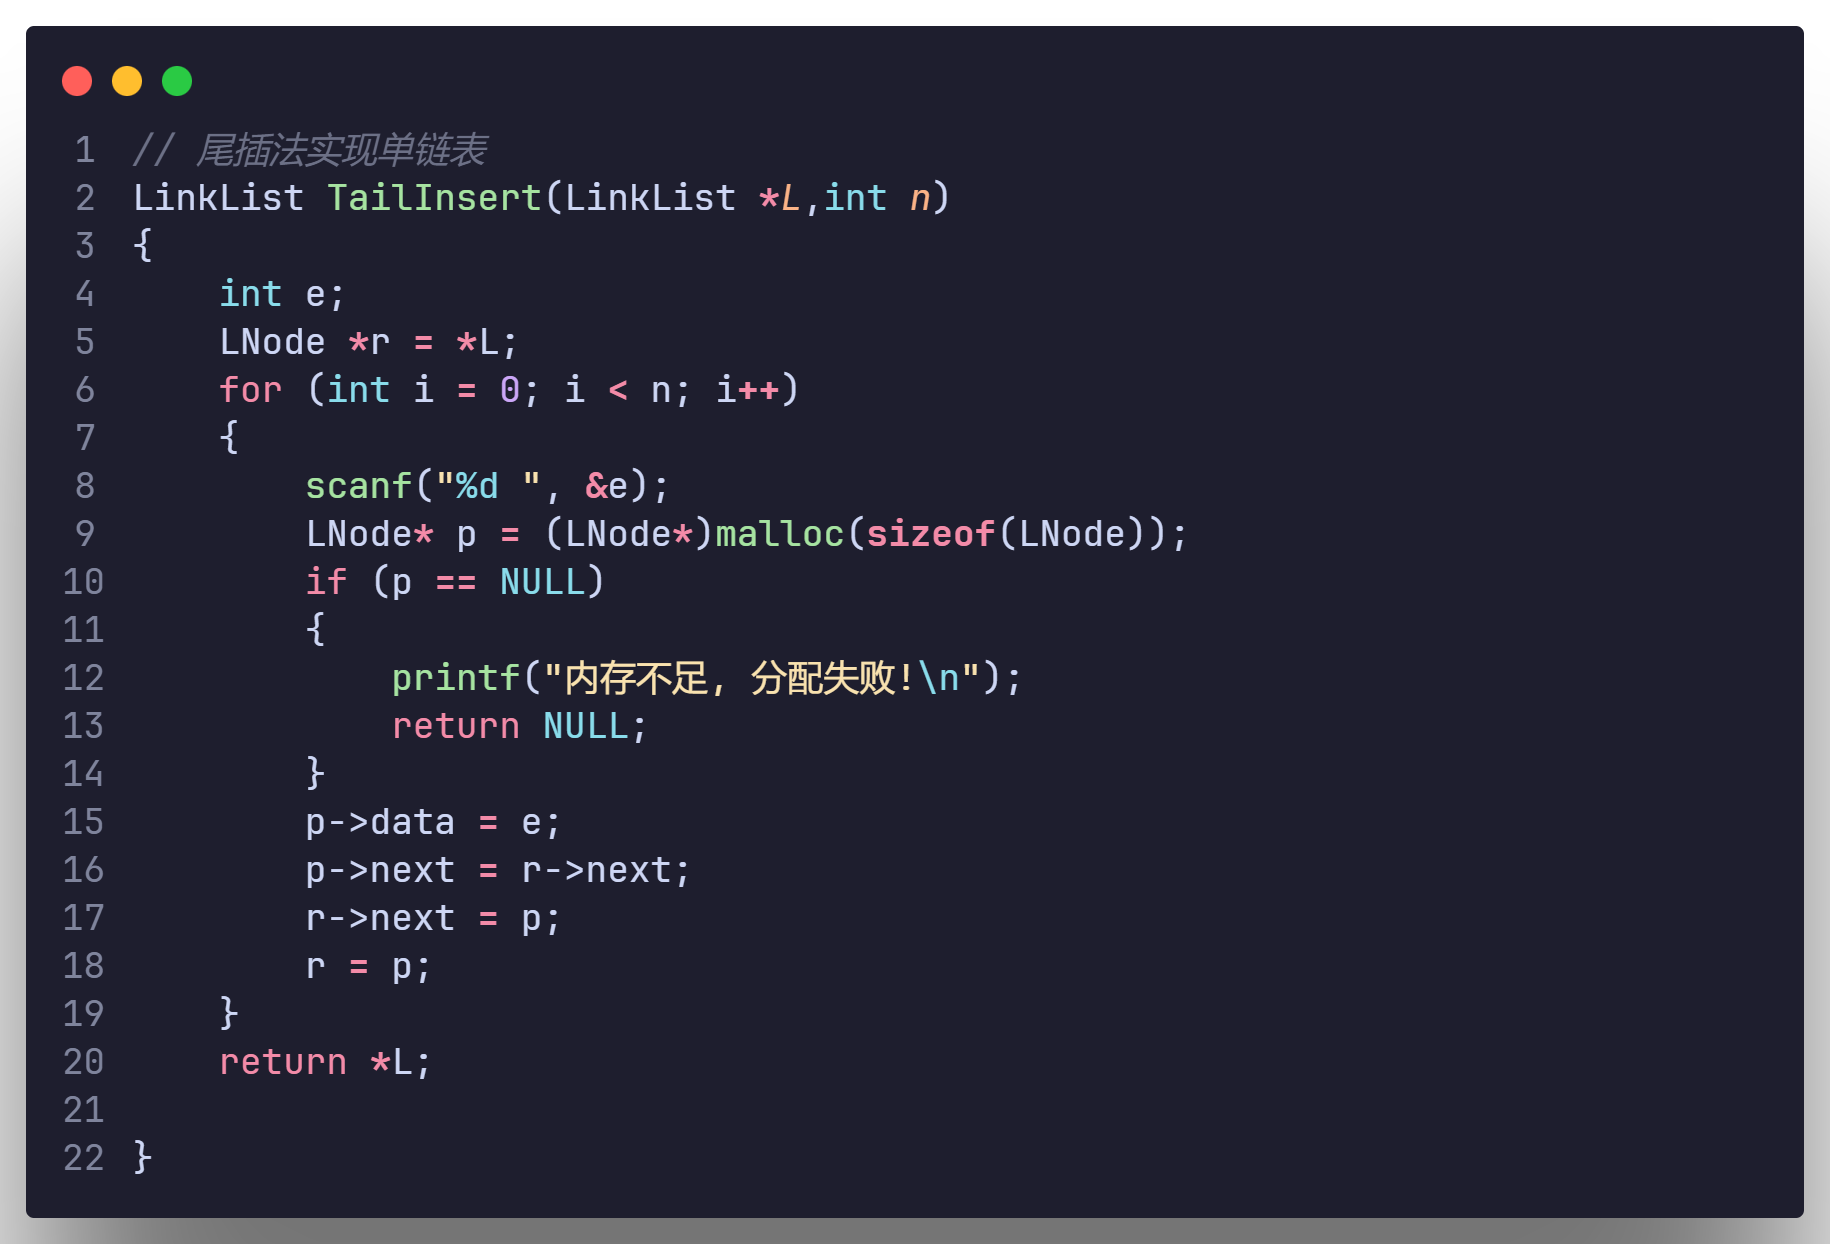
\includegraphics[scale=0.2]{"figure/Note/LinearList/SlTInsert.png"}
\end{figure}

\subsubsection{单链表反转}

\begin{figure}[H]
    \centering
    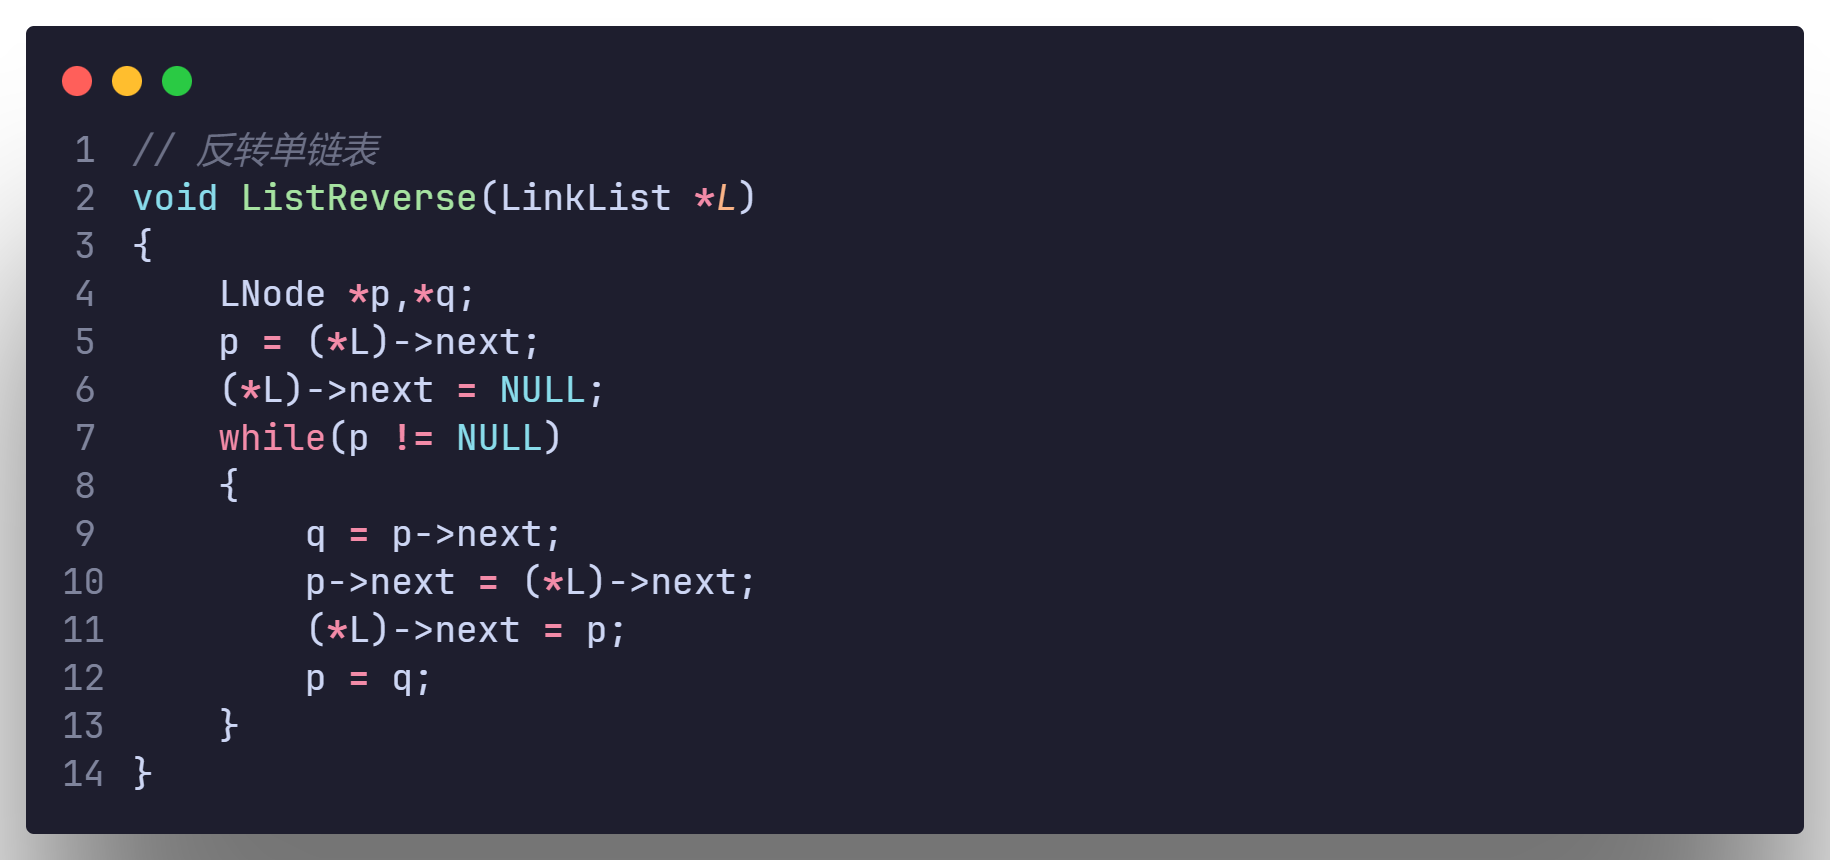
\includegraphics[scale=0.2]{"figure/Note/LinearList/SlReverse.png"}
\end{figure}



\subsection{双链表}
\begin{definition}[双链表]
    \begin{enumerate}
        \item 双链表有两个指针域,分别指向直接前驱和直接后继
        \item 头插法和尾插法的区别, 头插法实现反置
        \item 在插入和删除时,第一个和最后一个节点有特殊情况
    \end{enumerate}
\end{definition}

\subsubsection{双链表定义和函数声明}

\begin{figure}[H]
    \centering
    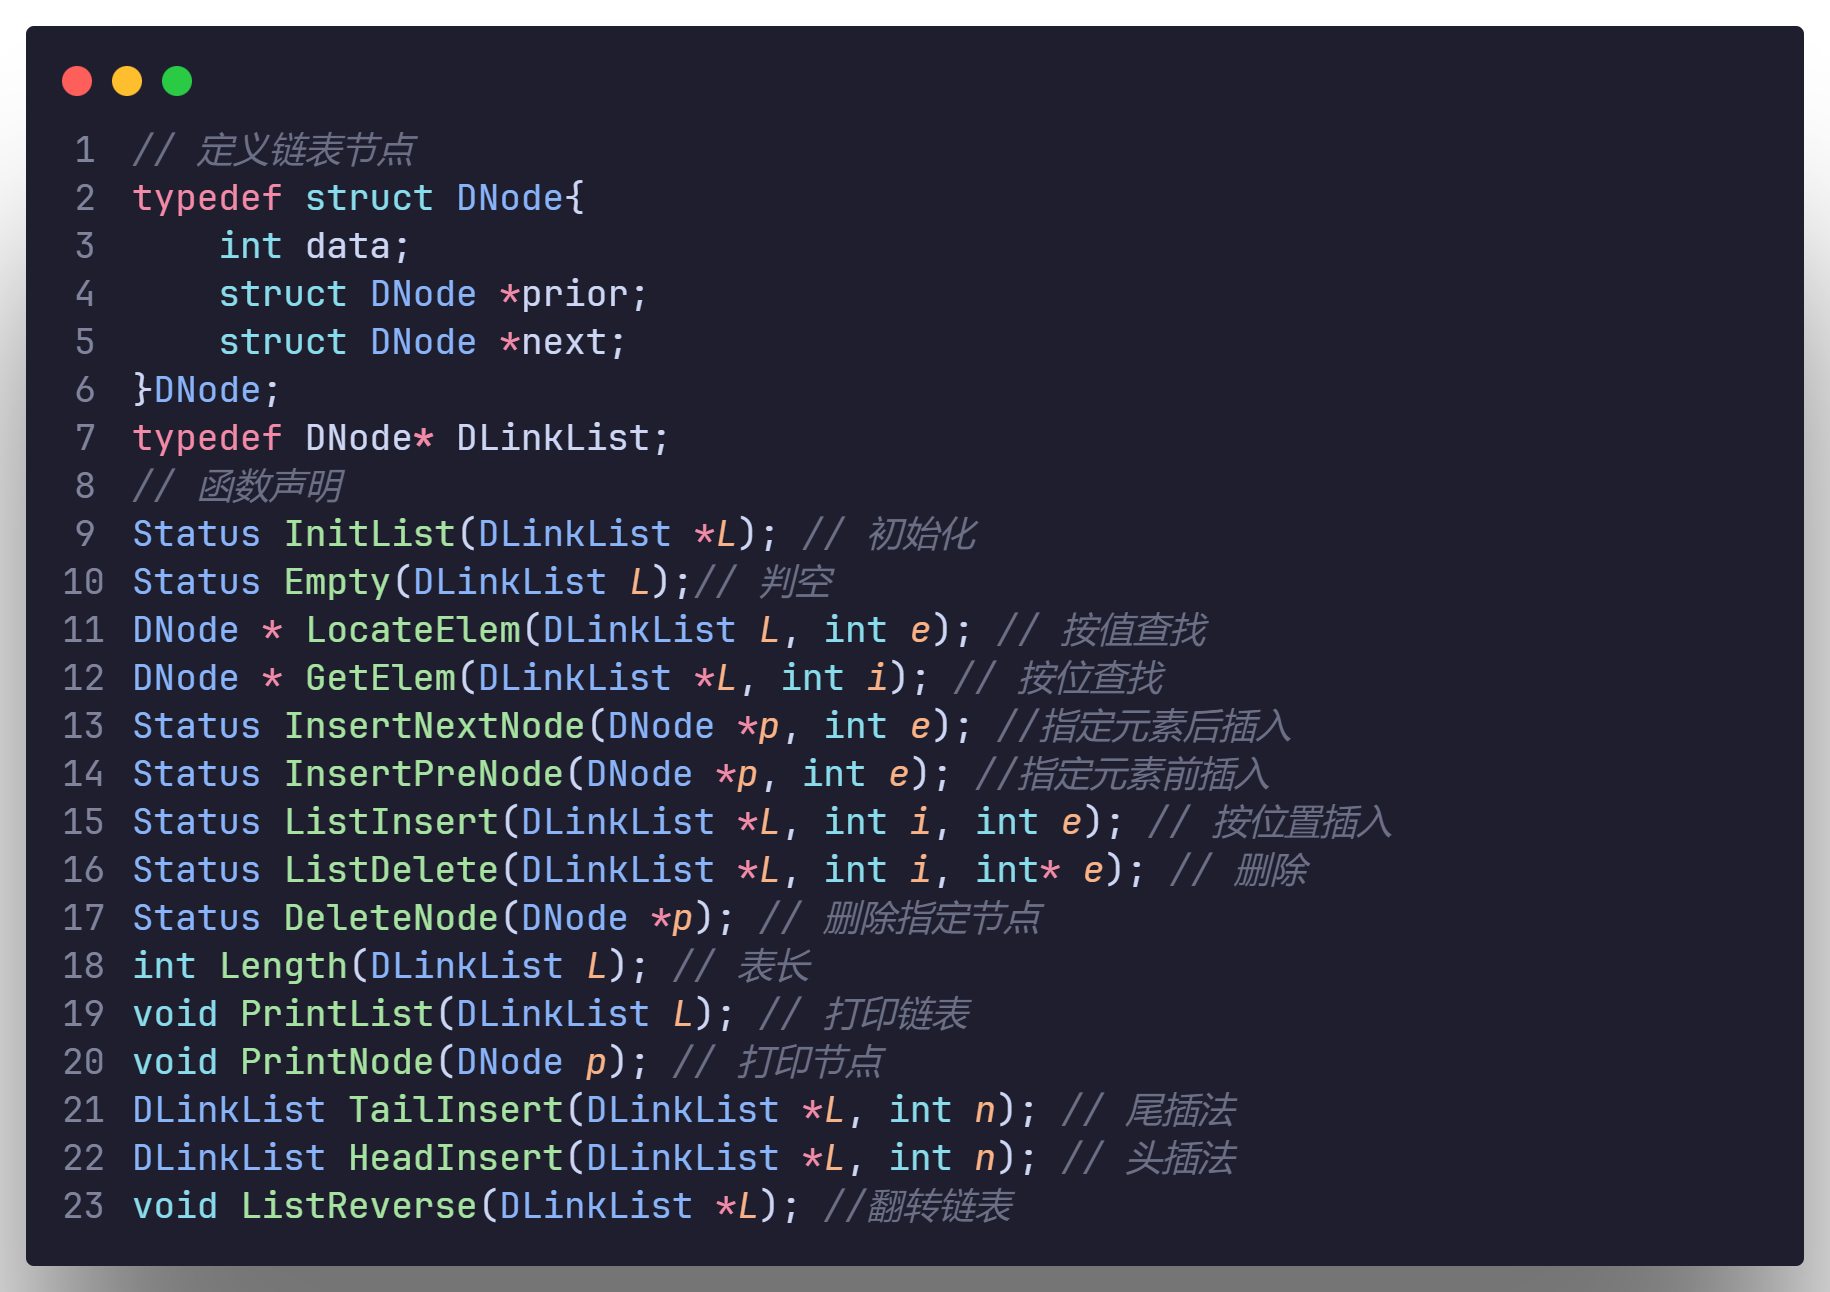
\includegraphics[scale=0.2]{"figure/Note/LinearList/DlFunction.png"}
\end{figure}

\subsubsection{双链表初始化}

\begin{figure}[H]
    \centering
    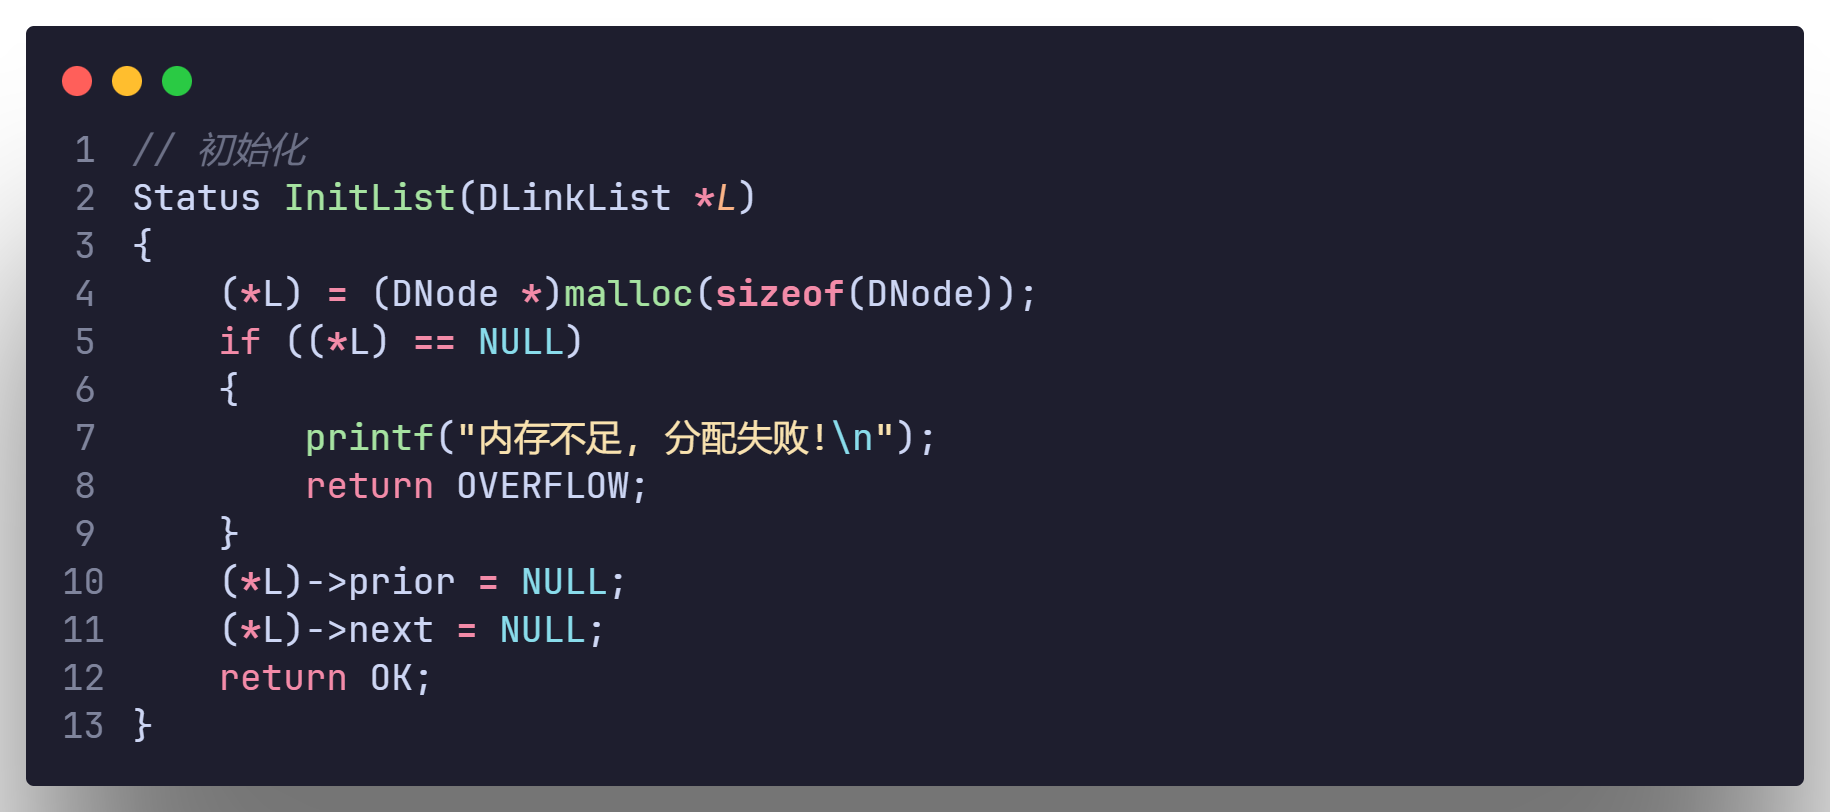
\includegraphics[scale=0.2]{"figure/Note/LinearList/DlInit.png"}
\end{figure}

\subsubsection{双链表查找}

(1). 按位置查找

\begin{figure}[H]
    \centering
    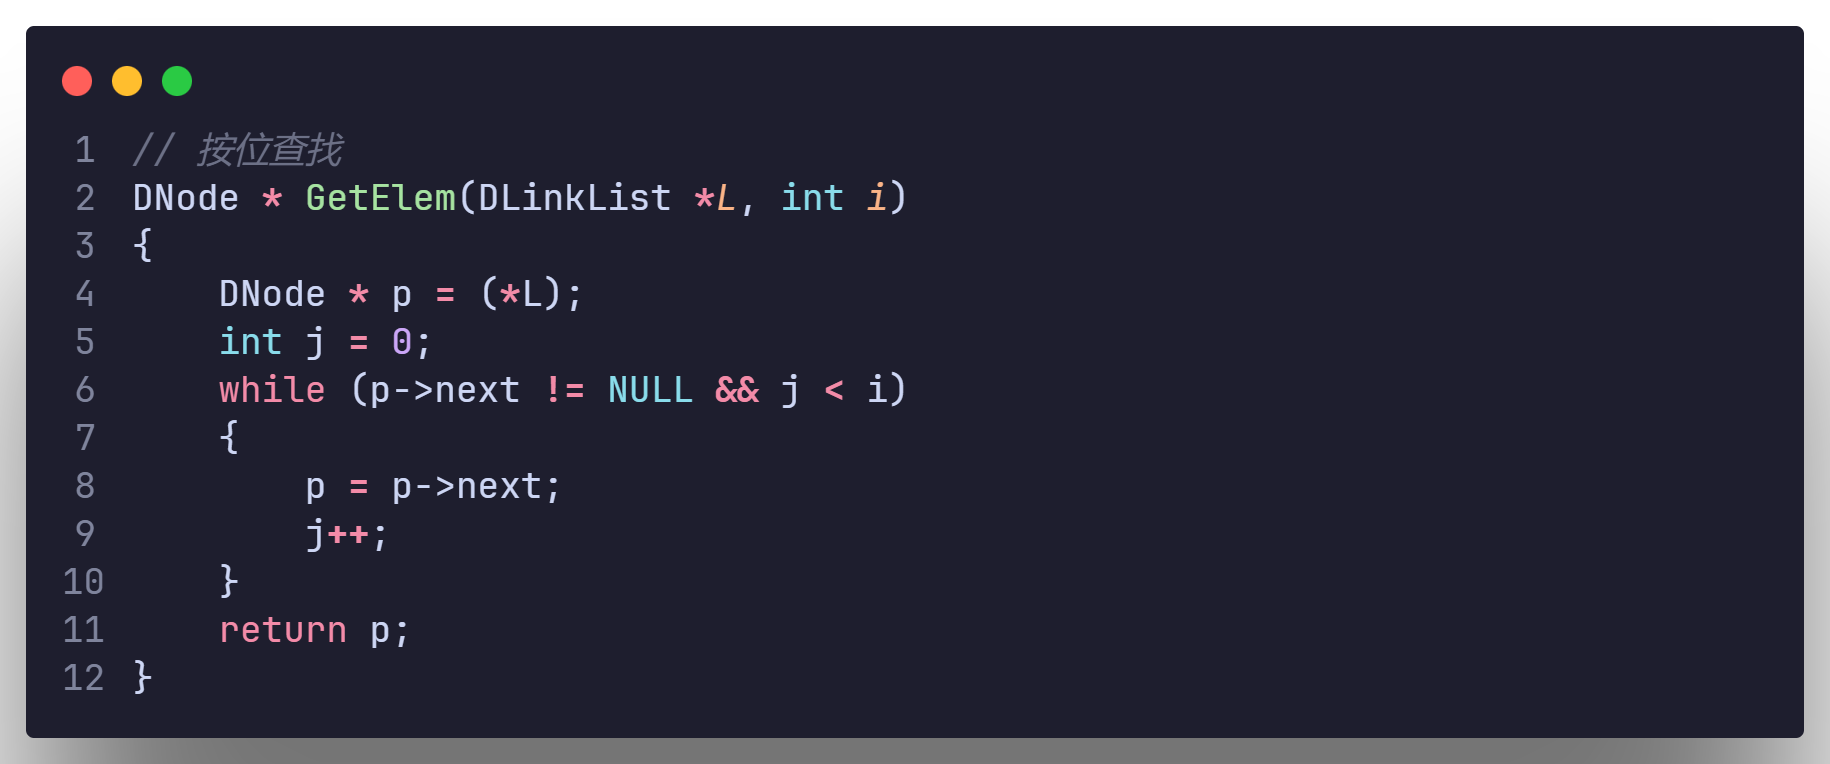
\includegraphics[scale=0.2]{"figure/Note/LinearList/DlNumSer.png"}
\end{figure}

(2). 按值查找

\begin{figure}[H]
    \centering
    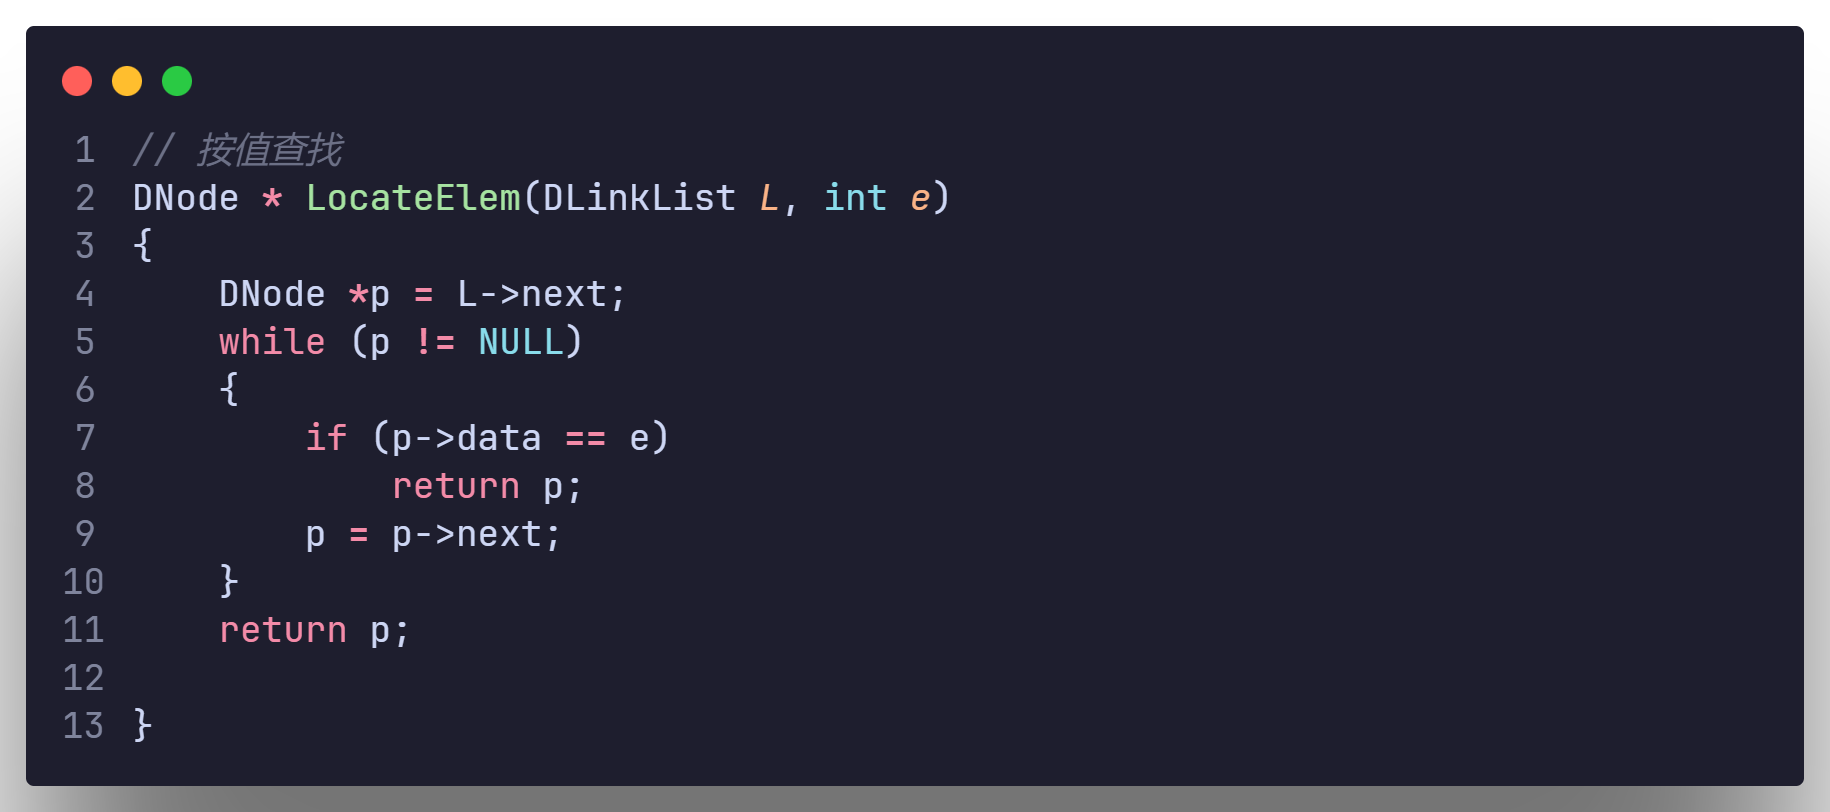
\includegraphics[scale=0.2]{"figure/Note/LinearList/DlItemSer.png"}
\end{figure}

\subsubsection{双链表插入}

(1). 指定元素后插入

\begin{figure}[H]
    \centering
    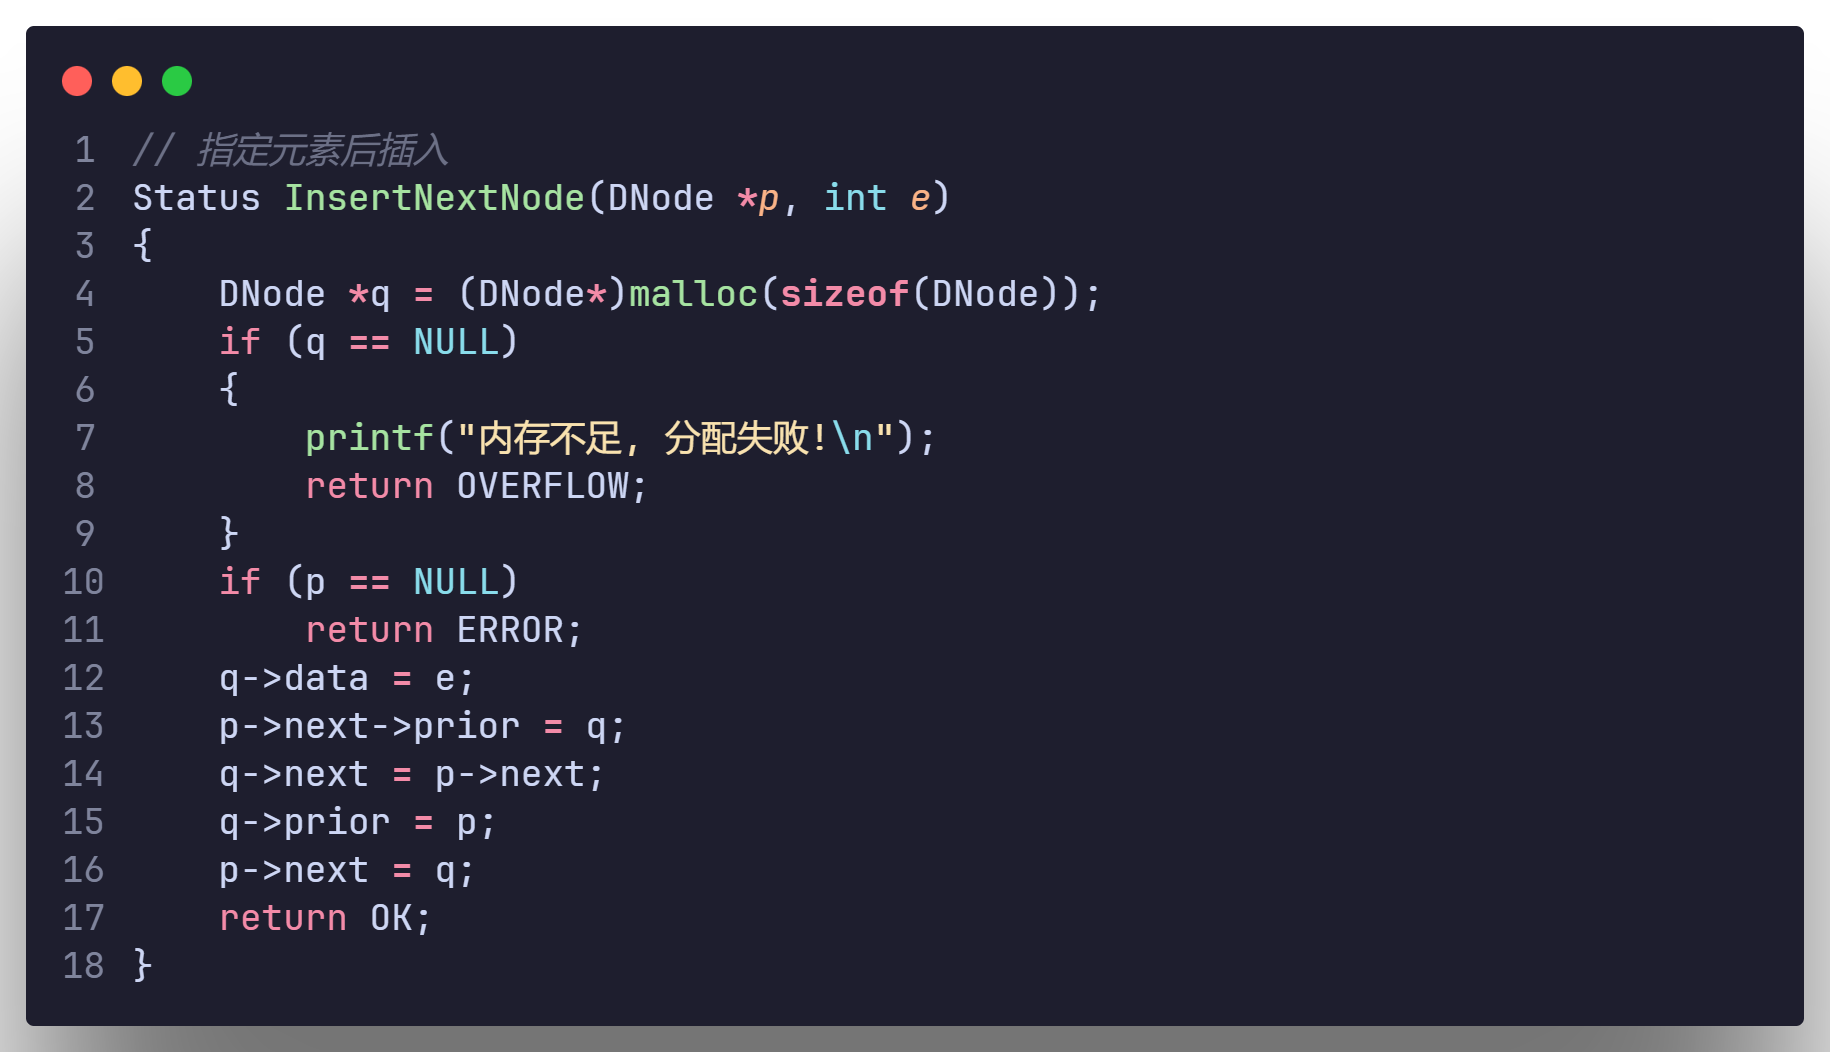
\includegraphics[scale=0.2]{"figure/Note/LinearList/DlBInsert.png"}
\end{figure}

(2). 指定元素前插入

\begin{figure}[H]
    \centering
    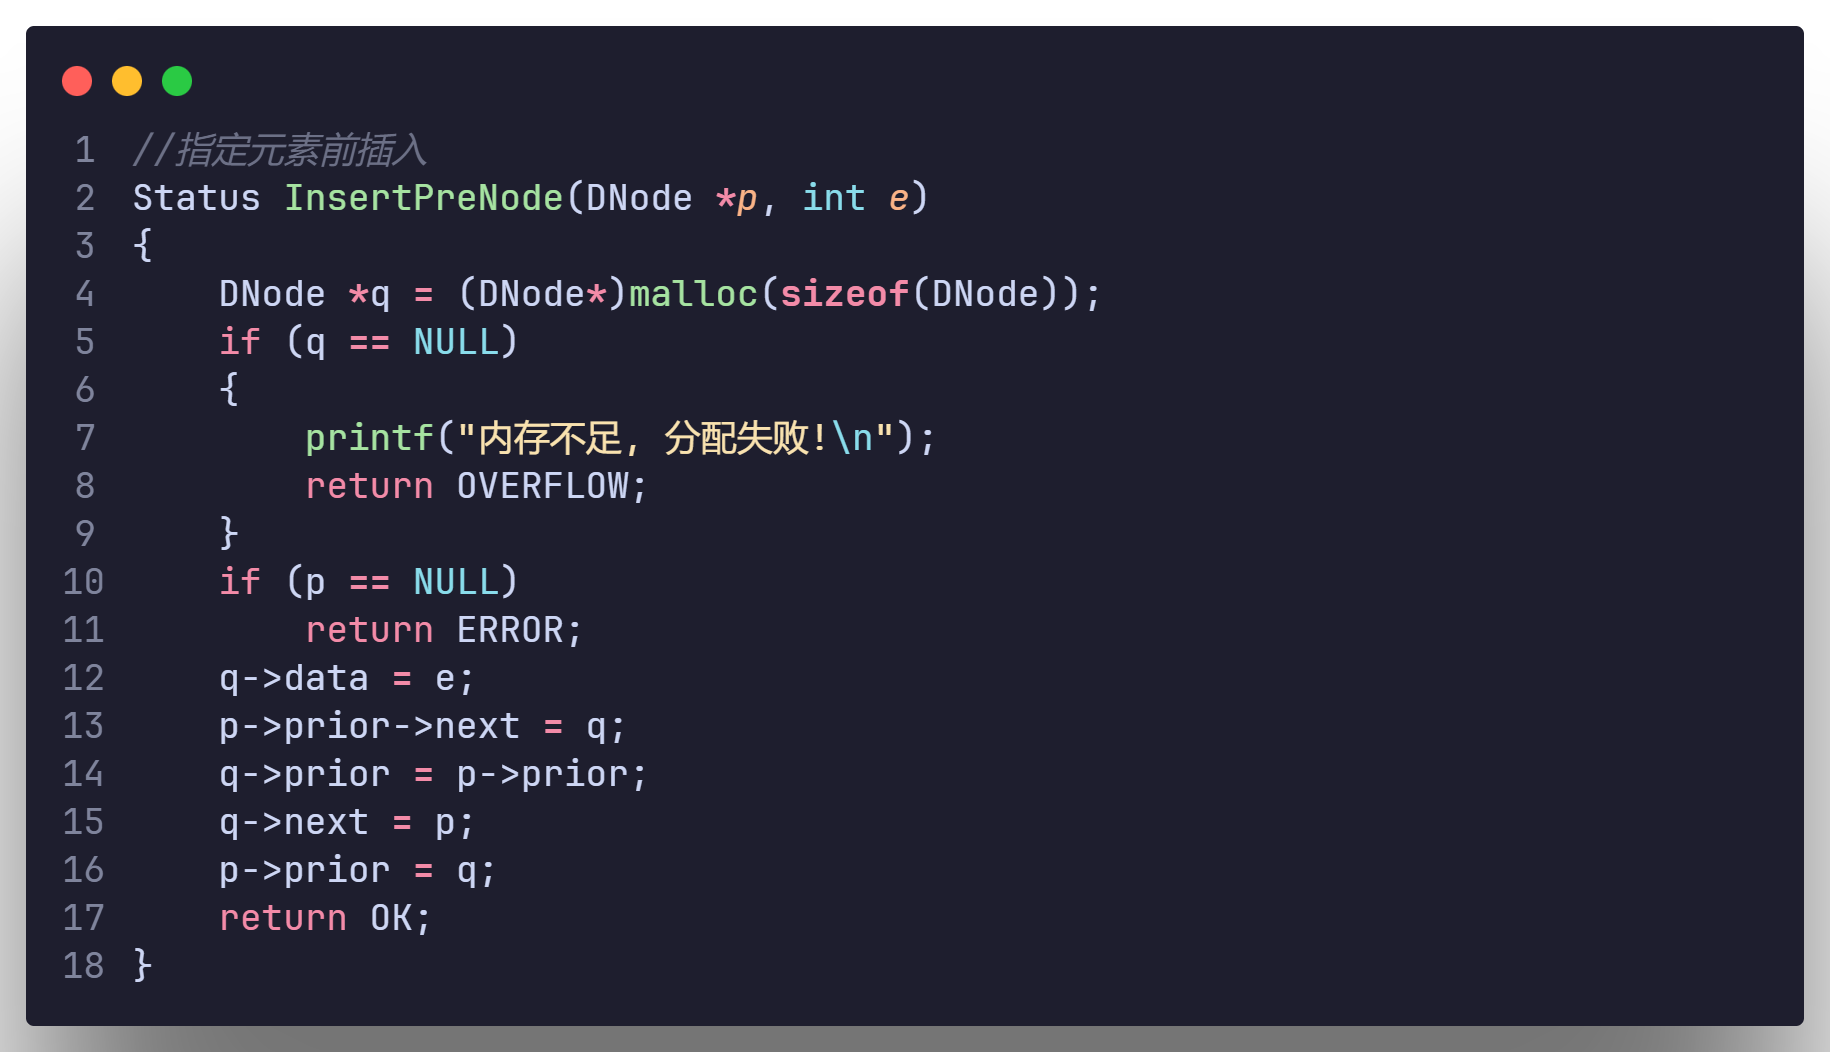
\includegraphics[scale=0.2]{"figure/Note/LinearList/DlFInsert.png"}
\end{figure}

(3). 指定位置插入

\begin{figure}[H]
    \centering
    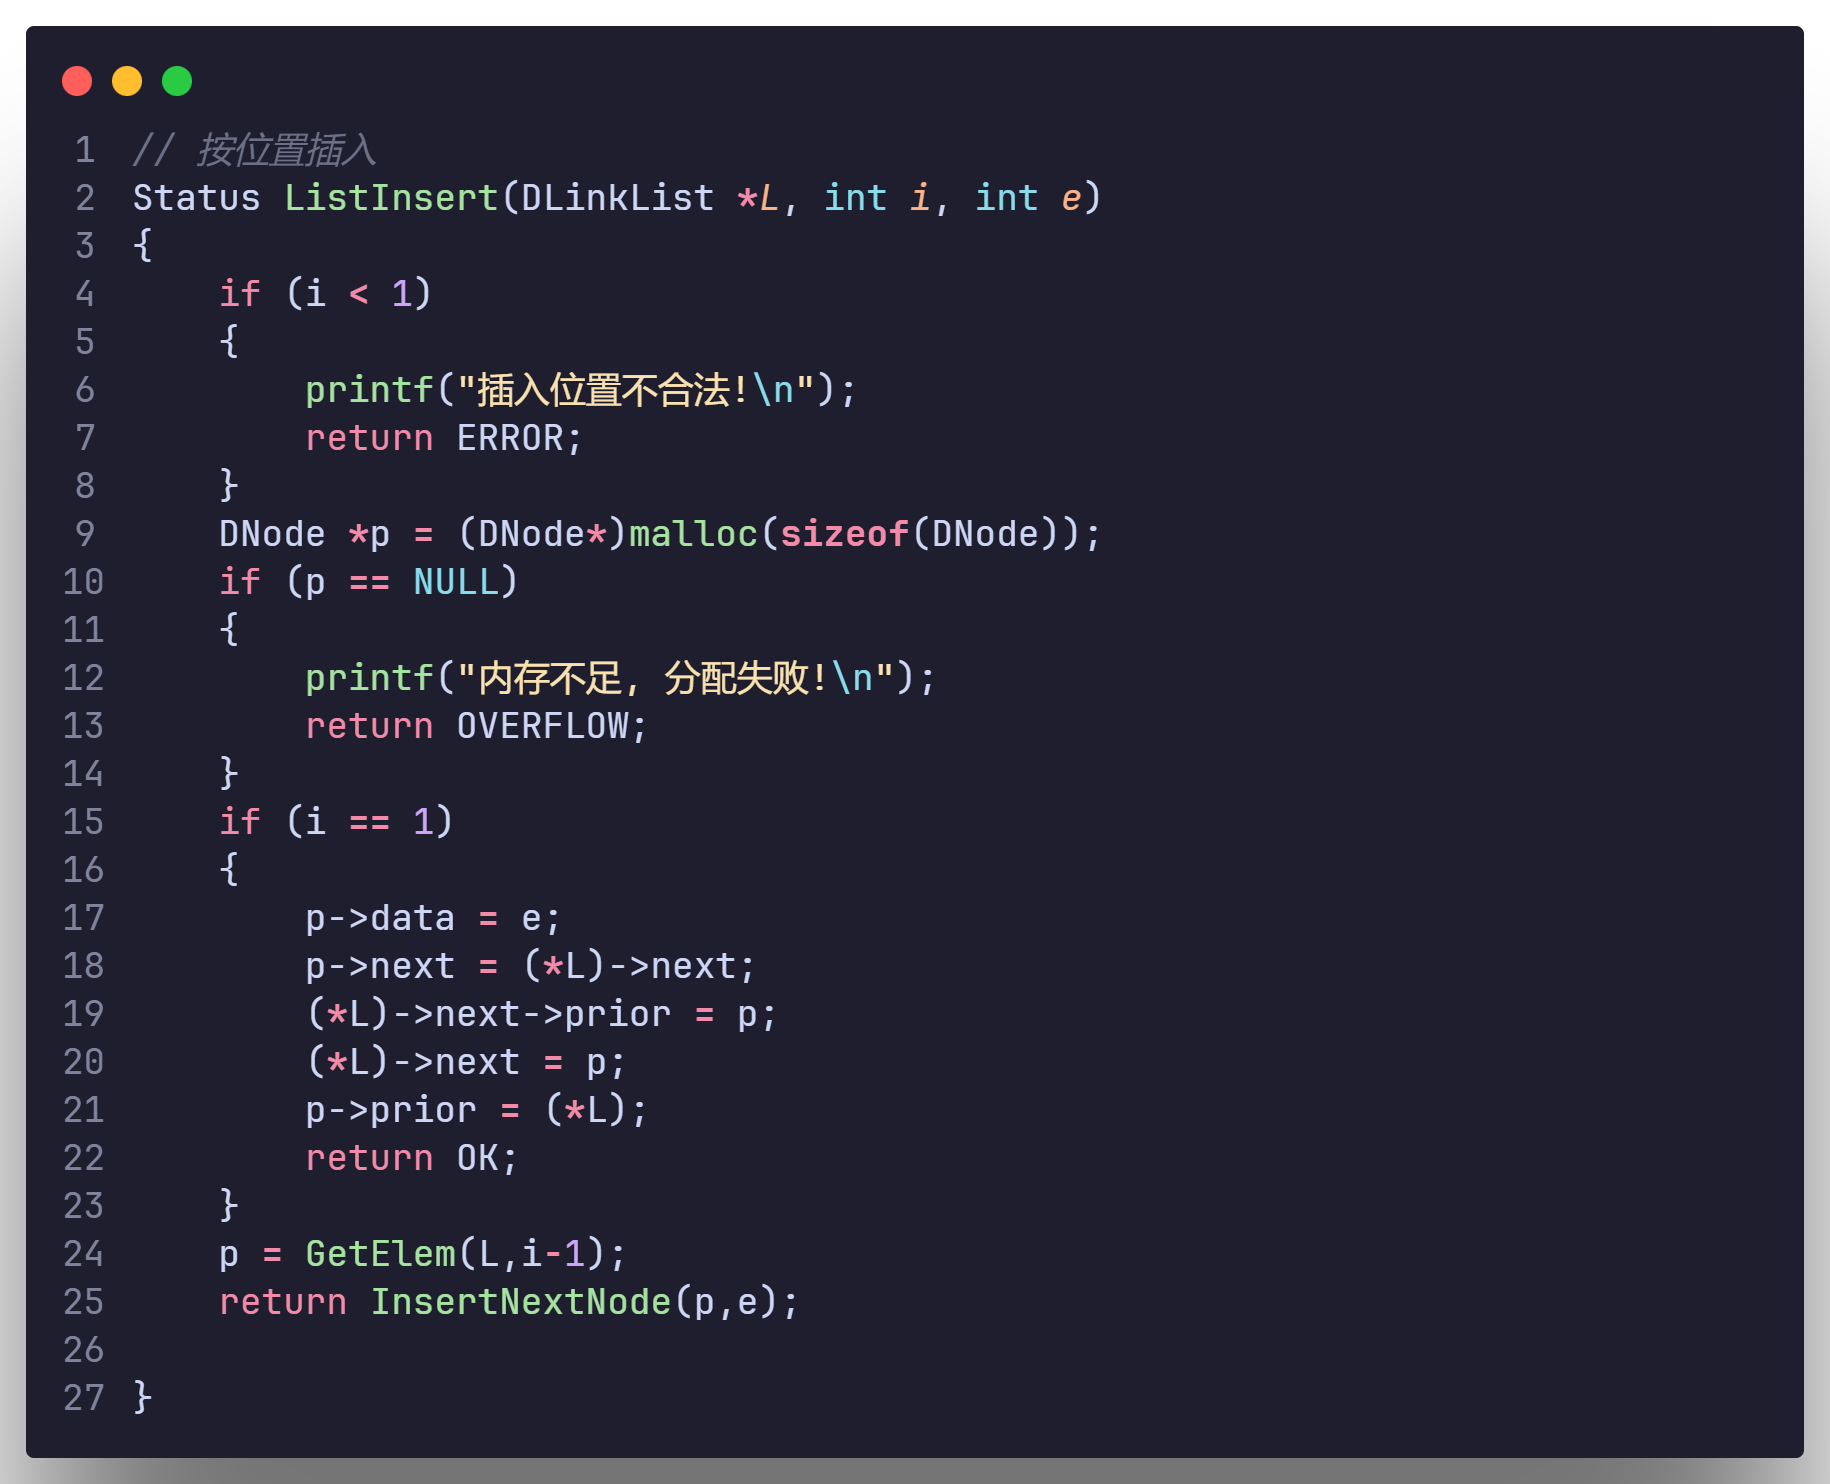
\includegraphics[scale=0.2]{"figure/Note/LinearList/DlInsert.png"}
\end{figure}


\subsubsection{双链表删除}

\begin{figure}[H]
    \centering
    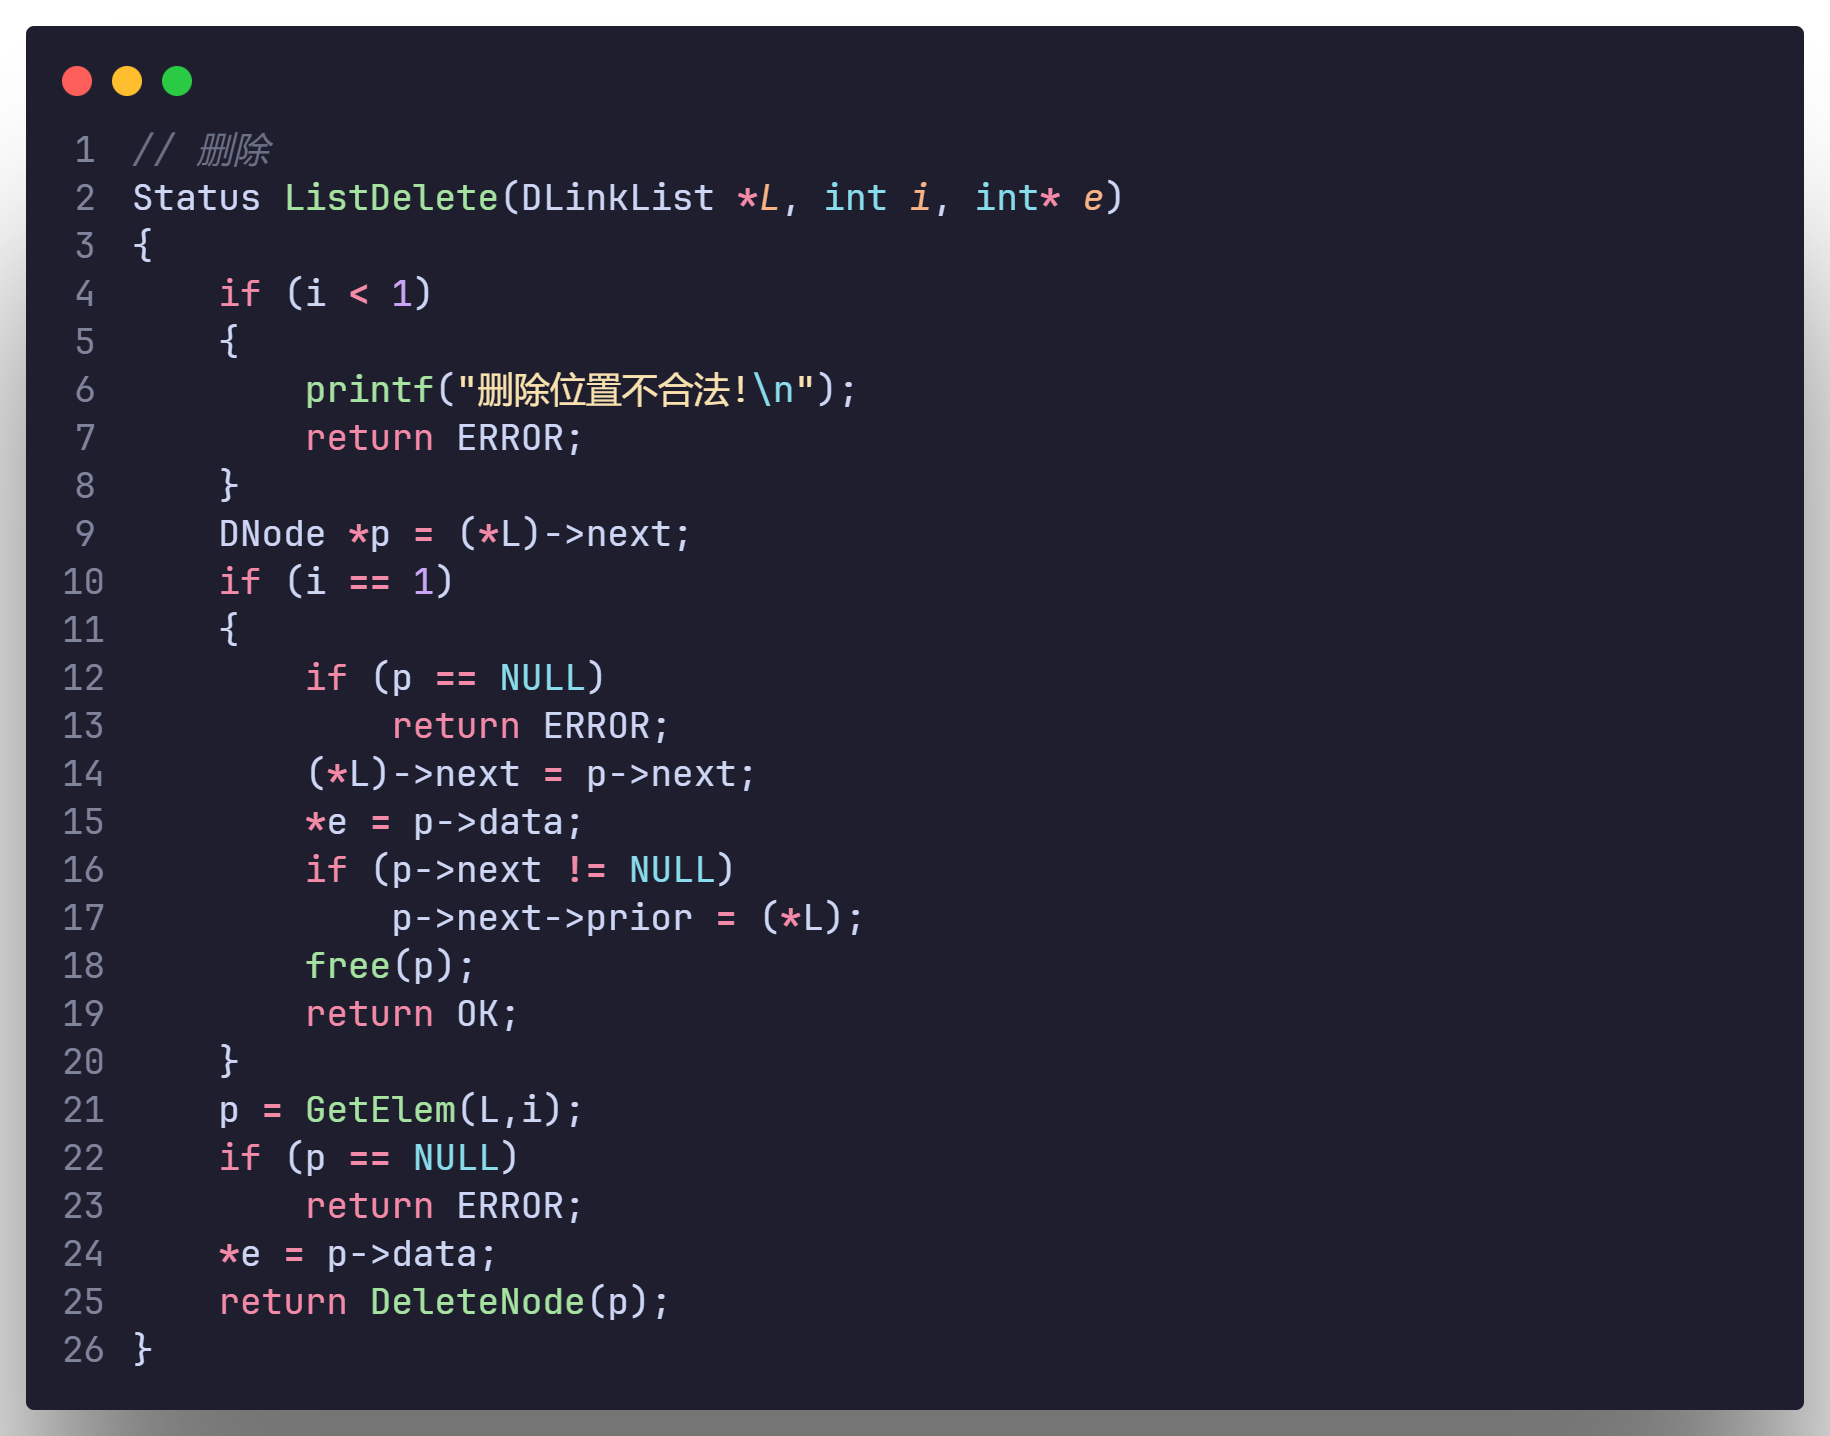
\includegraphics[scale=0.2]{"figure/Note/LinearList/DlDel.png"}
\end{figure}

\subsubsection{双链表辅助函数}

(1). $Length$

\begin{figure}[H]
    \centering
    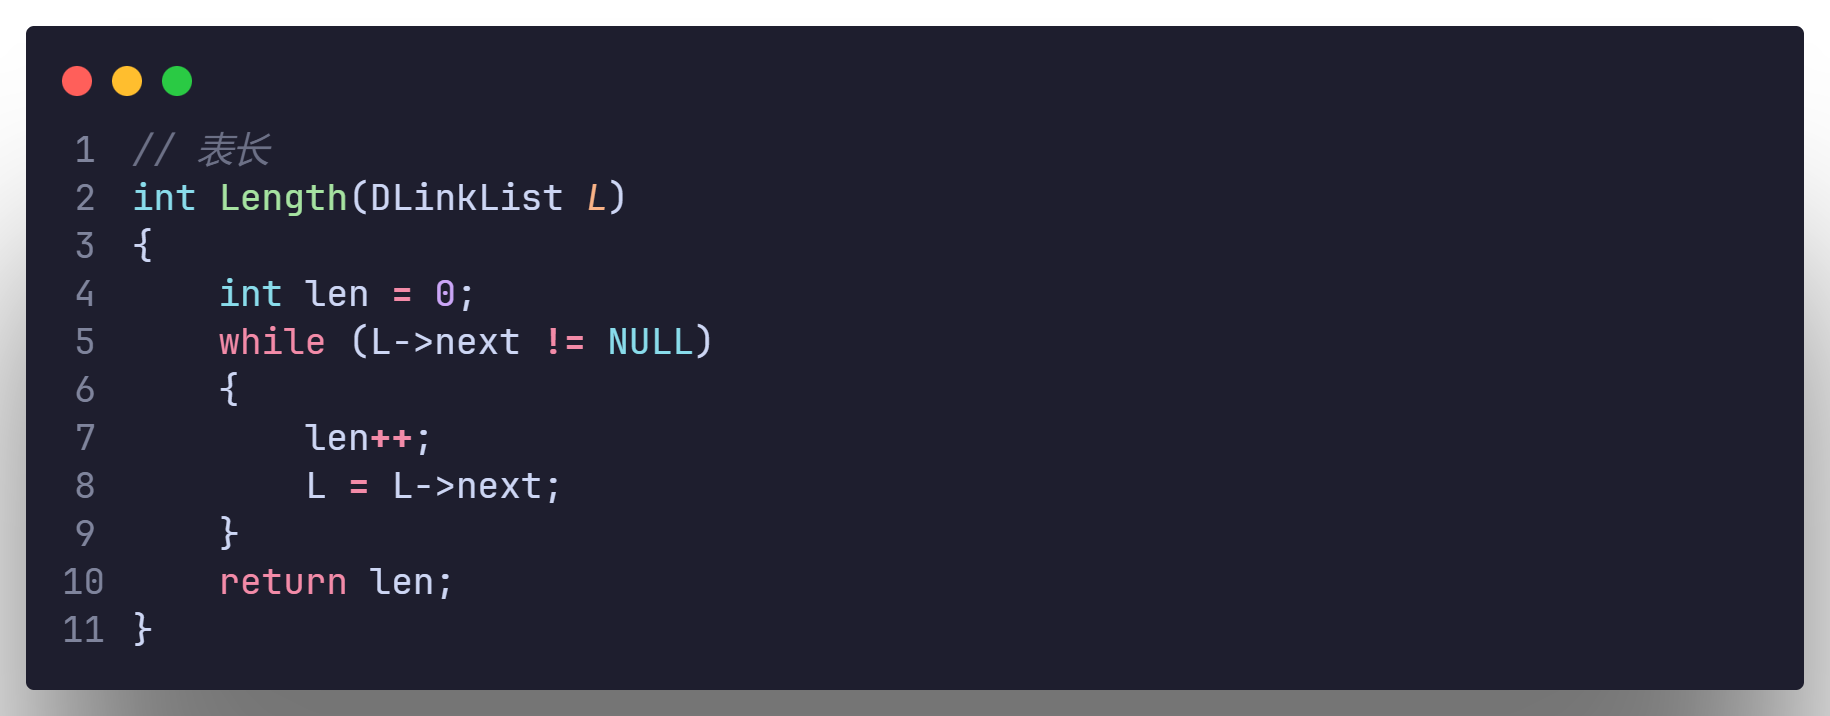
\includegraphics[scale=0.2]{"figure/Note/LinearList/DlLen.png"}
\end{figure}

(2). $Empty$

\begin{figure}[H]
    \centering
    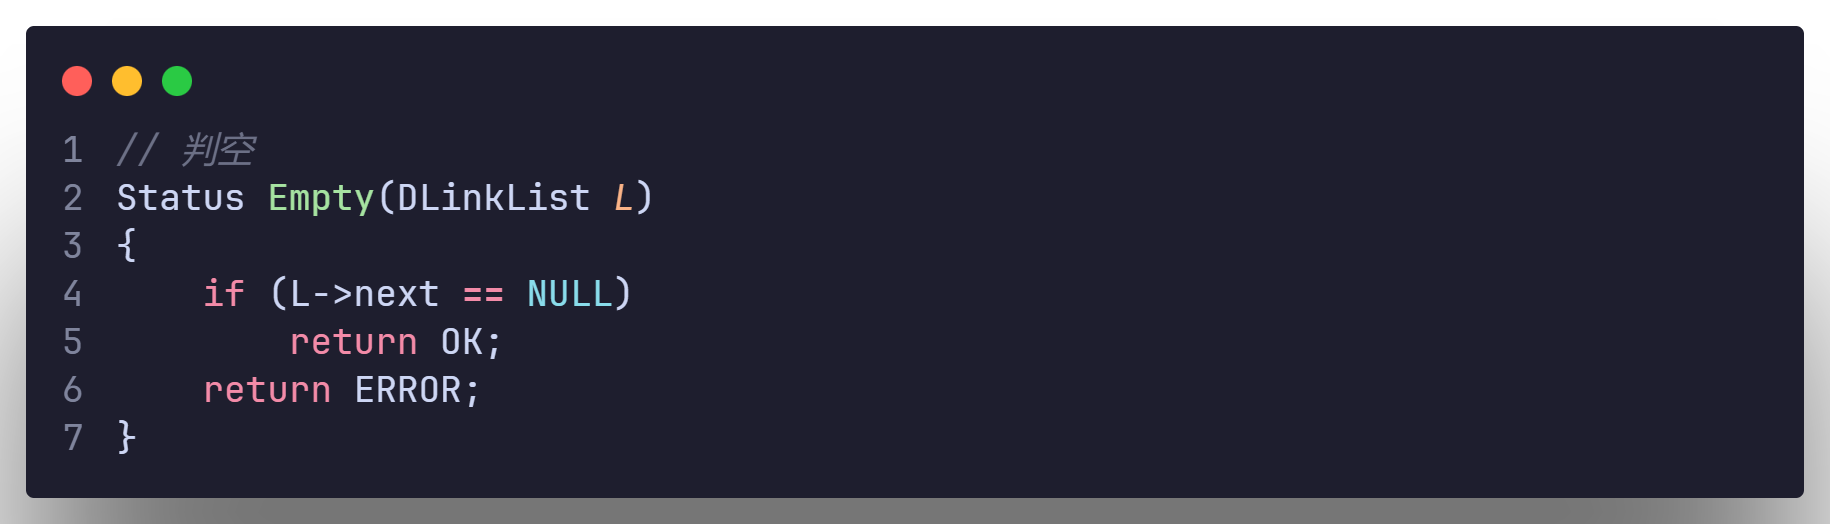
\includegraphics[scale=0.2]{"figure/Note/LinearList/DlEmpty.png"}
\end{figure}

(3). $PrintList$

\begin{figure}[H]
    \centering
    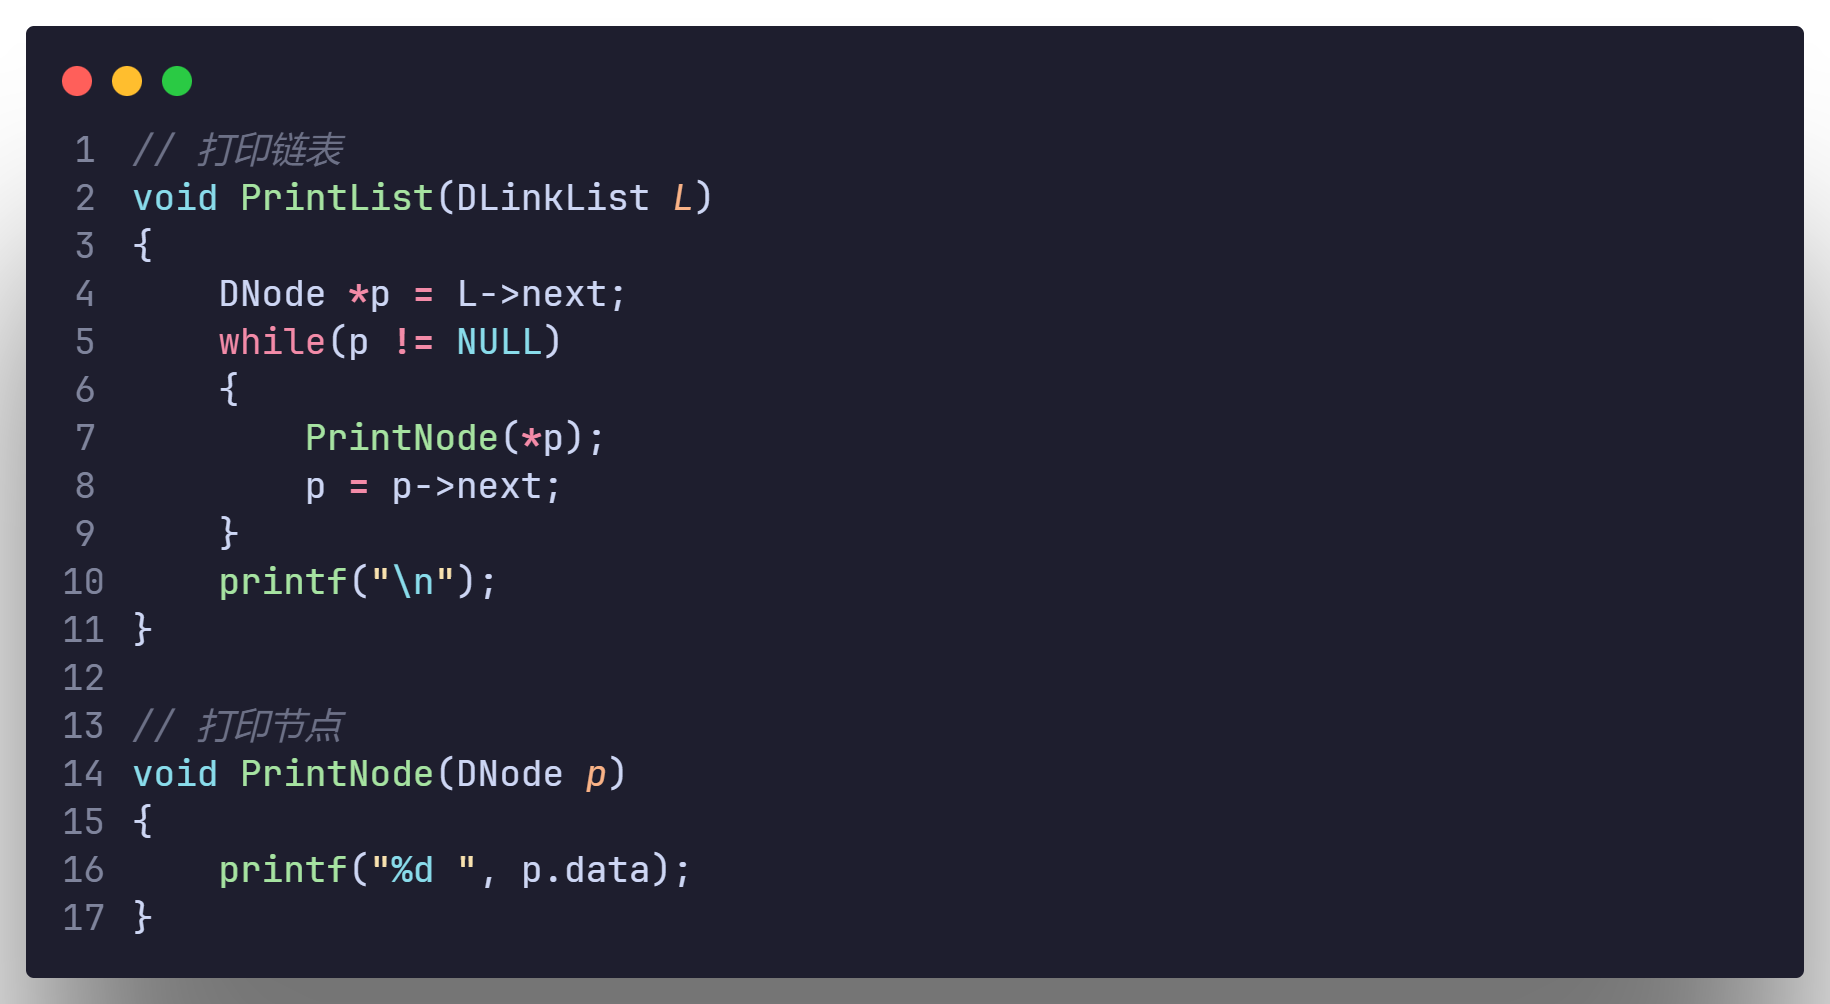
\includegraphics[scale=0.2]{"figure/Note/LinearList/DlPrint.png"}
\end{figure}

\subsubsection{头插法 \& 尾插法}

(1). 头插法

\begin{figure}[H]
    \centering
    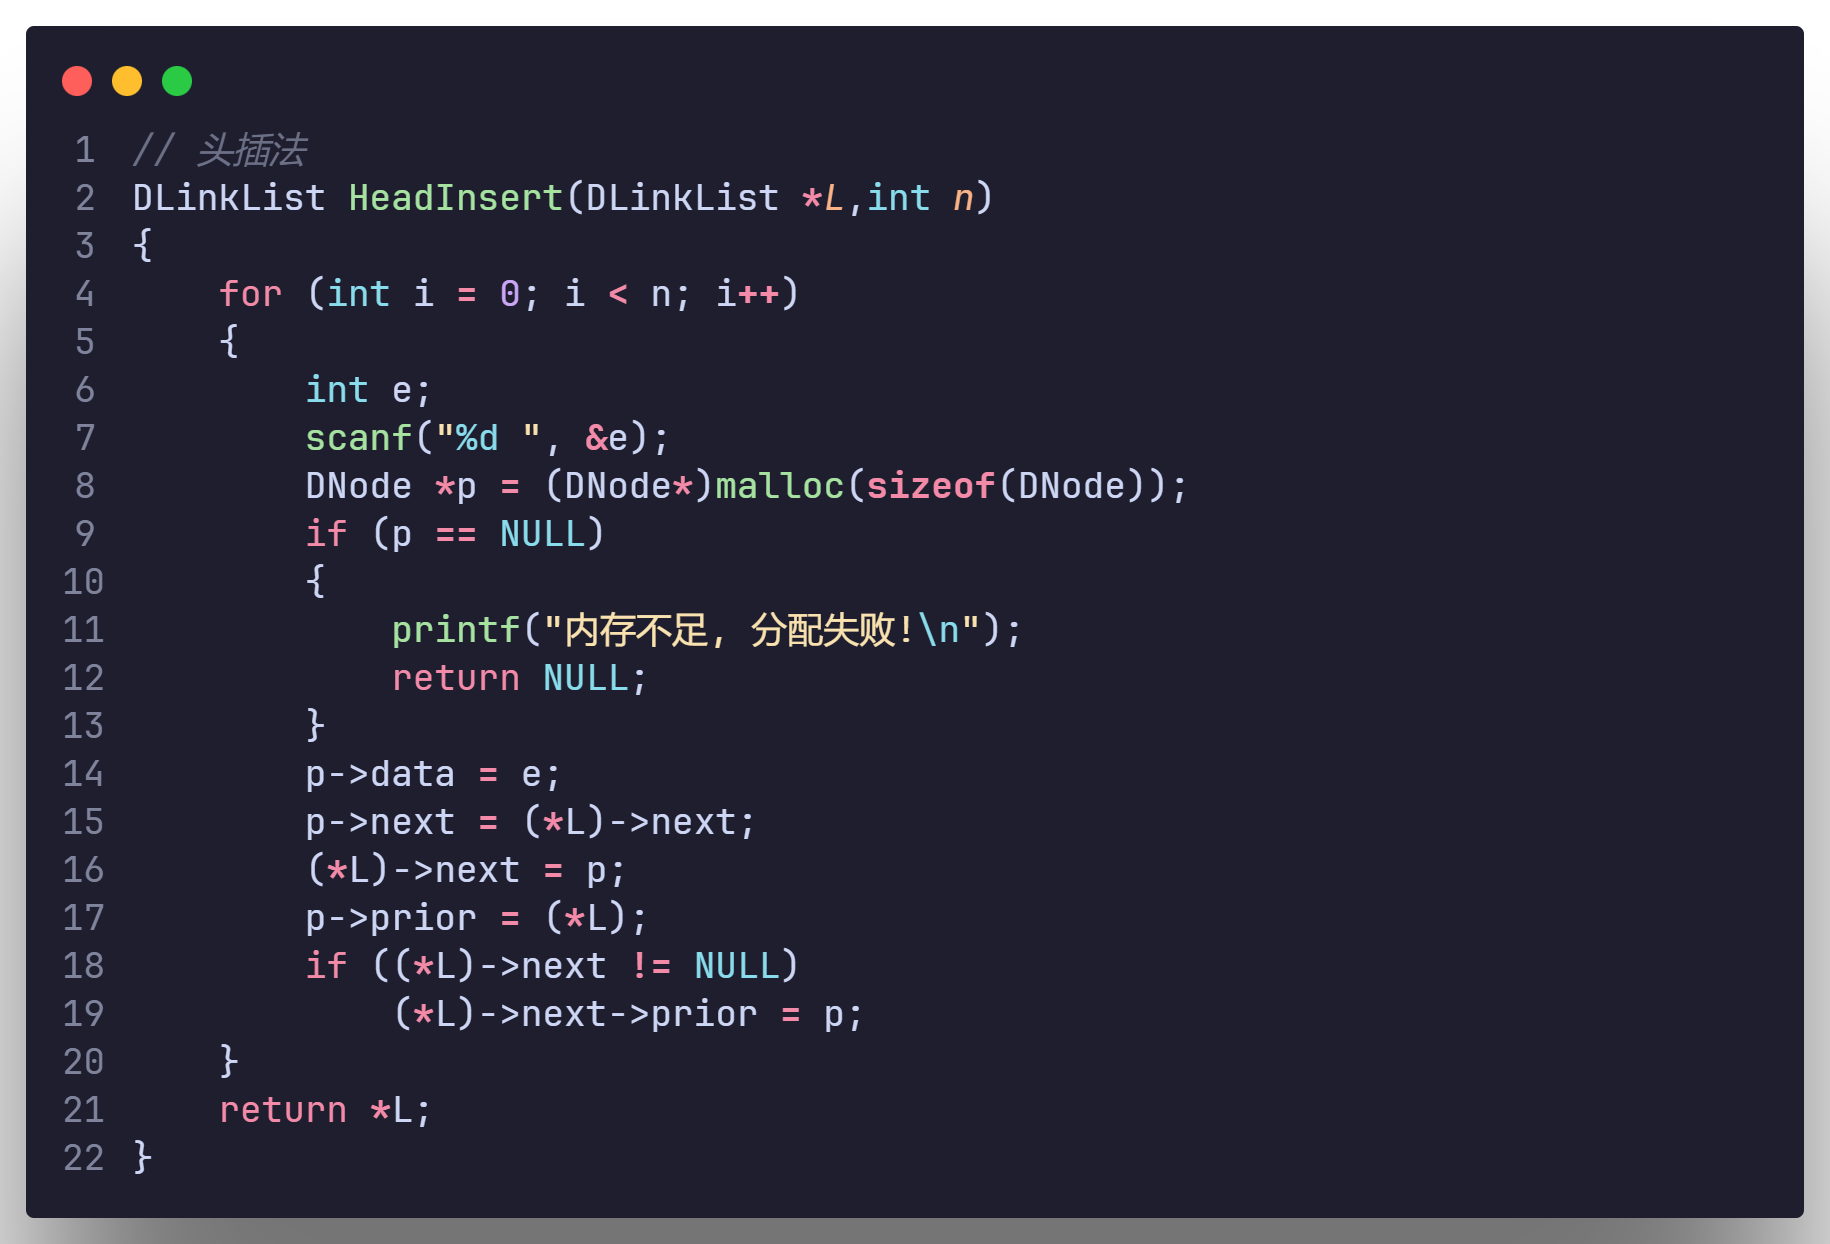
\includegraphics[scale=0.2]{"figure/Note/LinearList/DlHInsert.png"}
\end{figure}

(2). 尾插法

\begin{figure}[H]
    \centering
    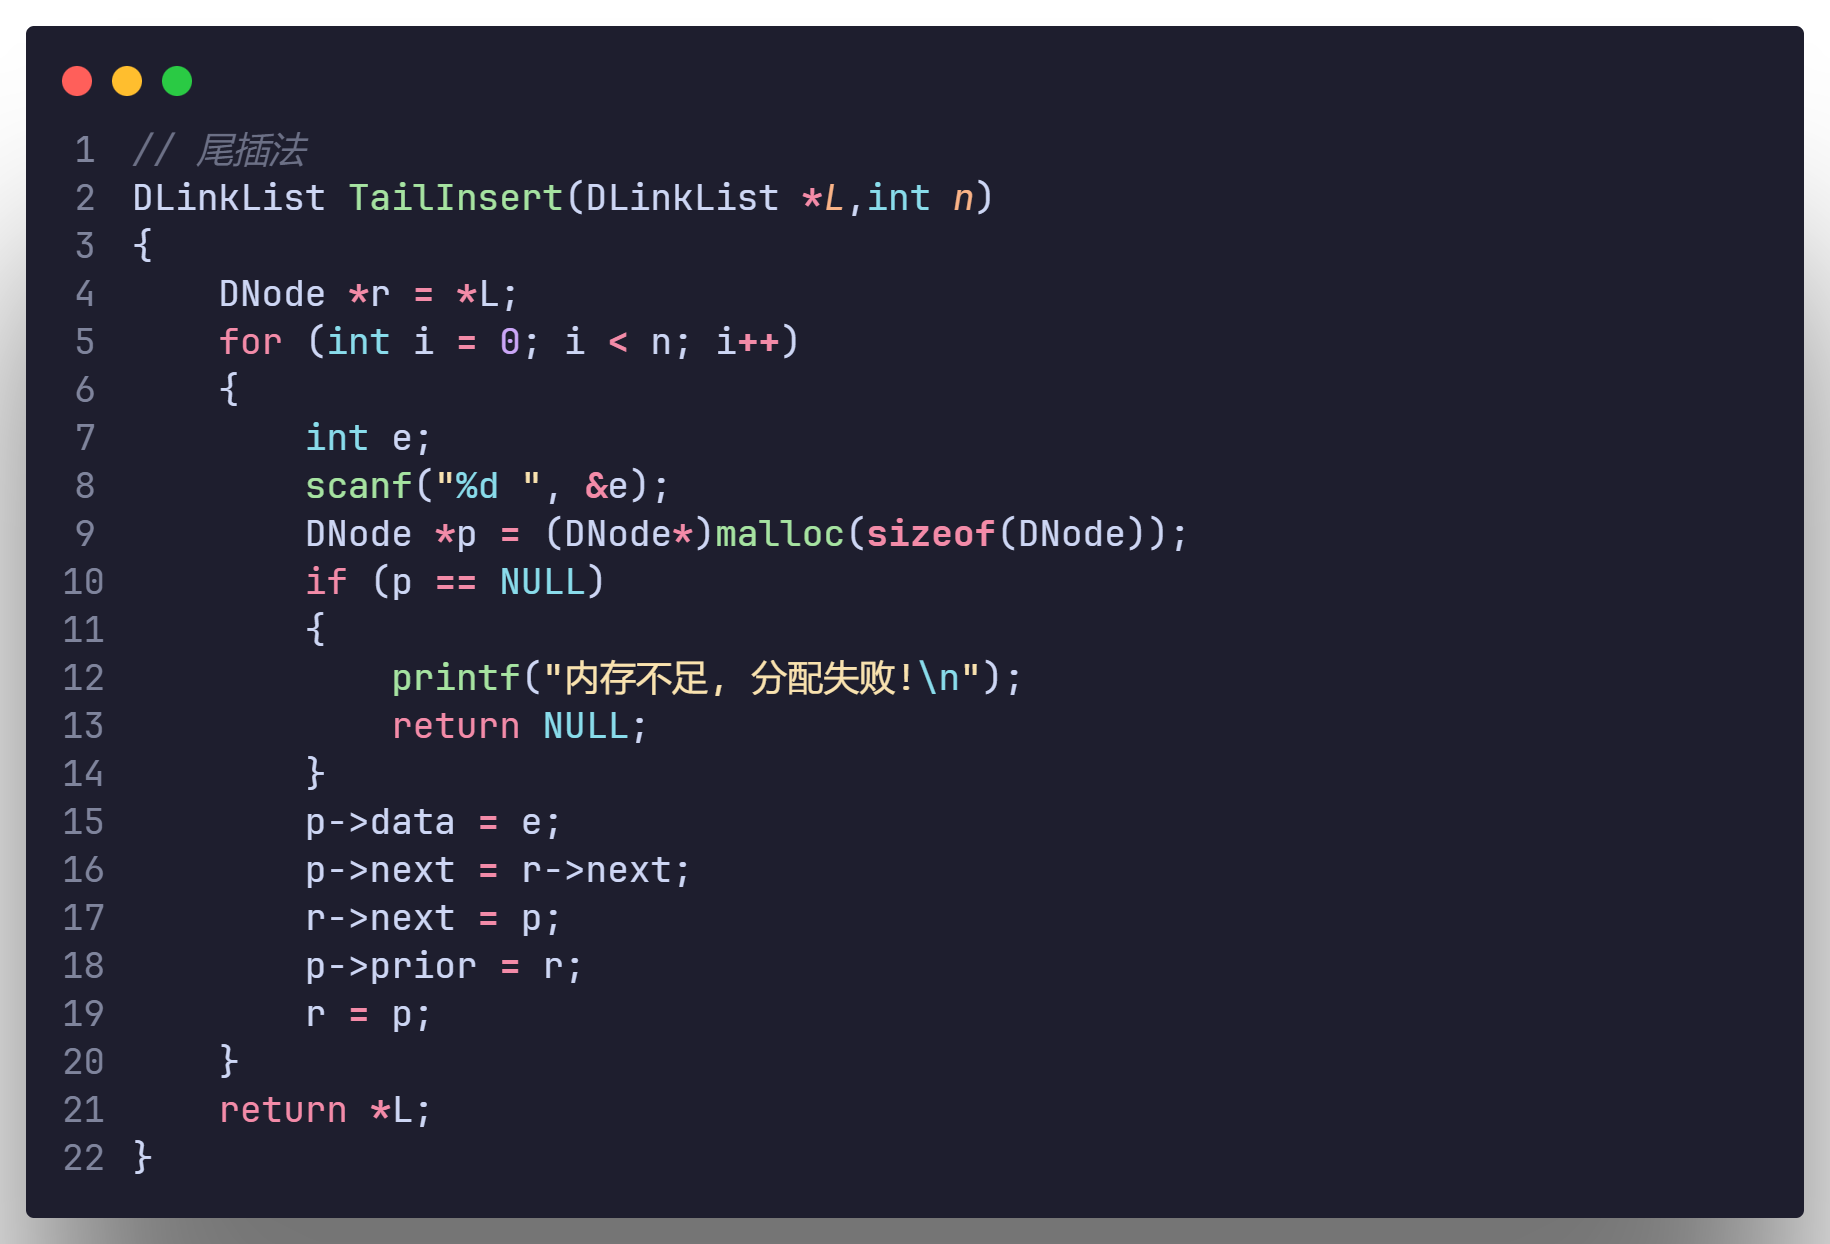
\includegraphics[scale=0.2]{"figure/Note/LinearList/DlTInsert.png"}
\end{figure}

\subsubsection{双链表反转}

\begin{figure}[H]
    \centering
    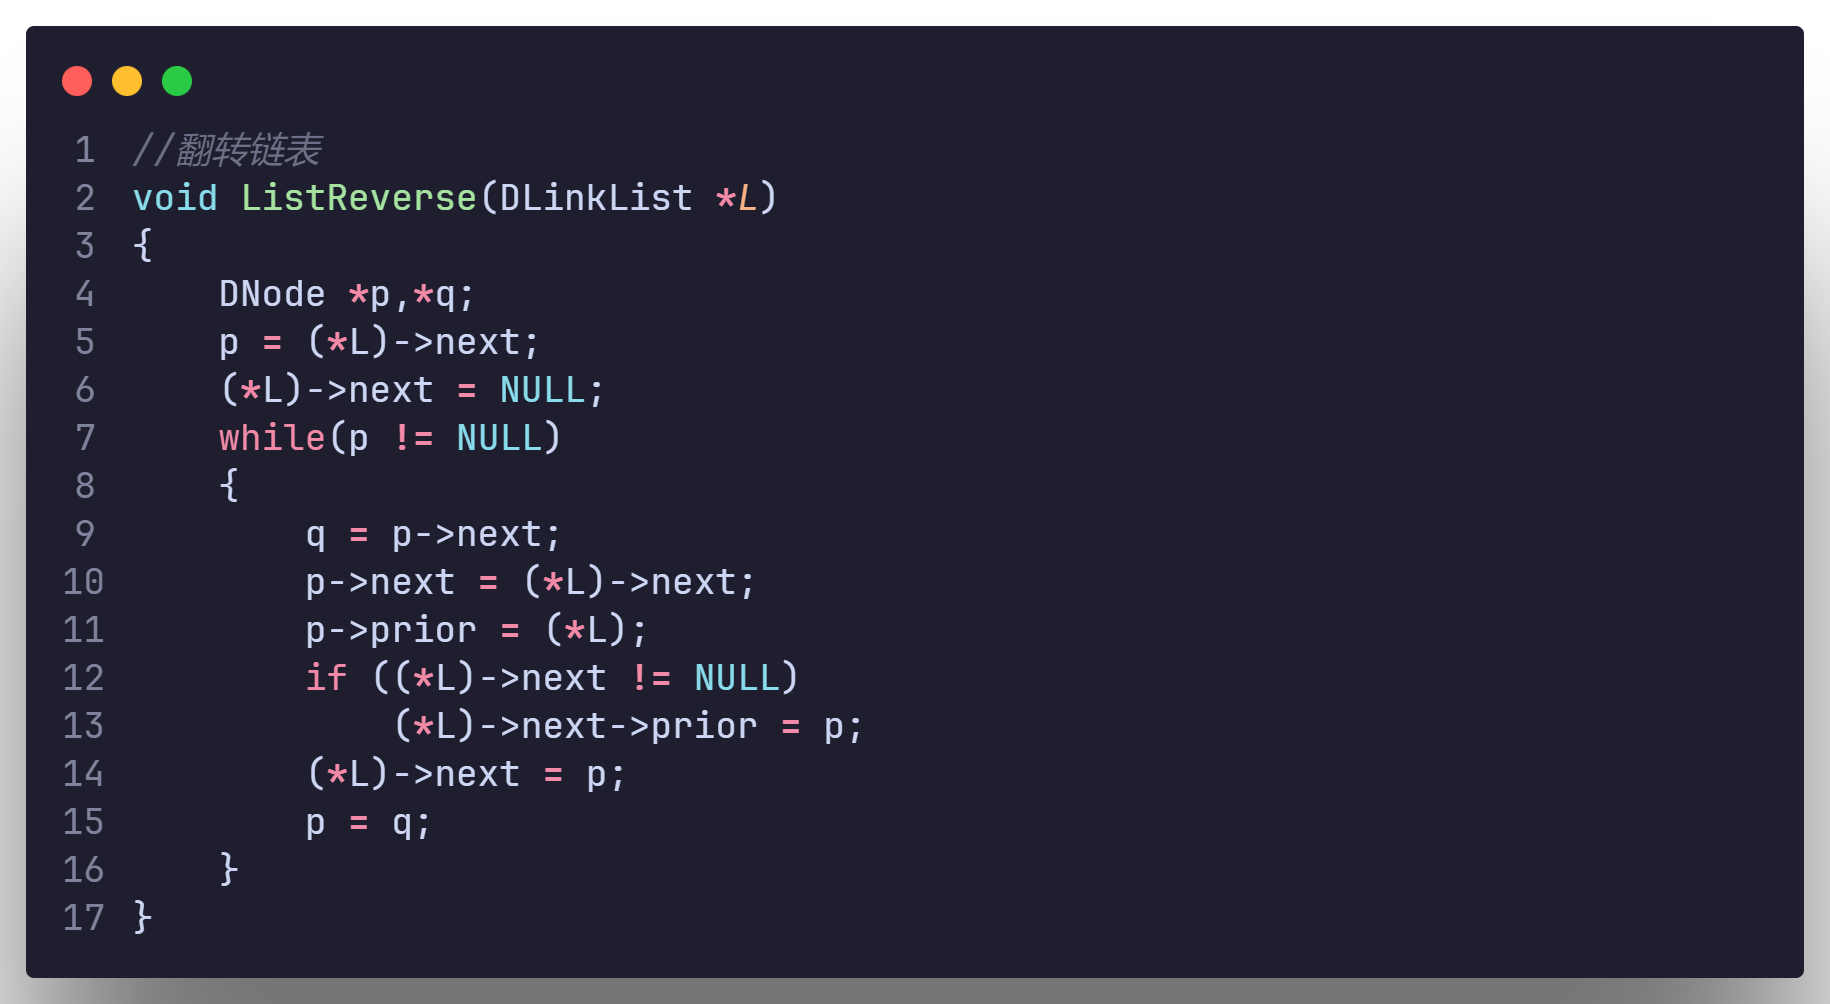
\includegraphics[scale=0.2]{"figure/Note/LinearList/DlReverse.png"}
\end{figure}


\subsection{循环链表}
\begin{definition}[循环链表]
    \begin{enumerate}
        \item 分为循环单链表和循环双链表, 与单链表和双链表的区别在于尾节点指向头节点
        \item 判空操作与单链表、双链表存在差异
        \item 插入、删除、以及判断表头、表尾节点有一定变化
    \end{enumerate}
\end{definition}

\subsection{静态链表}
\begin{definition}[静态链表]
    \begin{enumerate}
        \item 使用数组的链表, 数组第一个元素当做头节点, 每个位置除了保存数据元素外, 还保存下一个元素的位置
        \item 初始化时将所有位置的下一个元素位置清空
        \item 插入、删除操作需要找到上一个节点的位置, 然后将下一个元素位置清空
    \end{enumerate}
\end{definition}
\section{Summary}
\subsection{顺序表与链表比较}
\begin{table}[H]
    \centering
    \caption{顺序表与链表比较}
    \label{table: 顺序表与链表比较}
    \begin{tblr}{
        width = 0.8\textwidth,
        hlines = {1pt},
        hline{1,Z} = {2pt},
        vline{2-Y} = {1pt},
        cell{1}{1} = {r=1,c=2}{c},
        cell{1}{3} = {r=1,c=2}{c,teal7},
        cell{2}{1} = {r=2,c=1}{c},
        cell{2}{2} = {c},
        cell{2}{3} = {r=1,c=2}{l},
        cell{3}{2} = {c},
        cell{3}{3} = {r=1,c=2}{l},
        cell{4}{1} = {r=2,c=1}{c},
        cell{4}{2} = {c},
        cell{4}{3} = {r=1,c=2}{l},
        cell{5}{2} = {c},
        cell{5}{3} = {r=1,c=2}{l},
        cell{6}{1} = {r=2,c=2}{c},
        cell{6}{3} = {r=2,c=2}{l},
    }
    \diagbox{比较项目}{存储结构} &           & 顺序表                                                                  & \\
    空间                       & 存储空间   & {① 预先分配\\  ② 会导致空间闲置或溢出}                                      & \\
                              & 存储密度   & {① $\text{存储密度}=1$\\  ② 不需要额外空间来表示节点的逻辑关系}                & \\
    时间                       & 存取元素   &  {① 随机存取\\ ② 按位置访问元素时间复杂度 $O(1)$}                            & \\
                              & 插入、删除  &  平均移动一半的元素, 时间复杂度 $O(n)$                                      & \\
    适用情况                   &            & {① 表长变化不大,确定变化范围\\ ② 很少进行插入或删除, 经常按照元素位置序号访问数据} & \\
                              &           &                                                                         &\\
    \end{tblr}
    \myspace{1}
    \begin{tblr}{
        width = 0.8\textwidth,
        hlines = {1pt},
        hline{1,Z} = {2pt},
        vline{2-Y} = {1pt},
        cell{1}{1} = {r=1,c=2}{c},
        cell{1}{3} = {r=1,c=2}{c,blue7},
        cell{2}{1} = {r=2,c=1}{c},
        cell{2}{2} = {c},
        cell{2}{3} = {r=1,c=2}{l},
        cell{3}{2} = {c},
        cell{3}{3} = {r=1,c=2}{l},
        cell{4}{1} = {r=2,c=1}{c},
        cell{4}{2} = {c},
        cell{4}{3} = {r=1,c=2}{l},
        cell{5}{2} = {c},
        cell{5}{3} = {r=1,c=2}{l},
        cell{6}{1} = {r=2,c=2}{c},
        cell{6}{3} = {r=2,c=2}{l},
    }
    \diagbox{比较项目}{存储结构} &           & 链表                                                            & \\
    空间                       & 存储空间   & {① 动态分配 \\  ② 不会出现空间闲置或溢出}                            & \\
                              & 存储密度   & {① $\text{存储密度}<1$\\ ② 需要借助指针来表示节点的逻辑关系}          &\\
    时间                       & 存取元素   & {① 顺序存取\\ ② 按位置访问元素时间复杂度 $O(n)$}                     &\\
                              & 插入、删除  & 不需要移动元素, 确定插入或删除位置后,时间复杂度 $O(n)$                 &\\
    适用情况                   &            &{① 表长变化很大\\ ② 频繁进行插入或删除操作}                            &\\
                              &           &                                                                 &\\
    \end{tblr}
\end{table}

\subsection{单链表、双链表、循环链表比较}
\begin{table}[H]
    \centering
    \caption{单链表、双链表、循环链表比较}
    \label{table: 单链表、双链表、循环链表比较}
    \small
    \begin{tblr}[m]{
        width = \textwidth,
        colsep = {0.5pt},
        hlines = {1pt},
        hline{1,Z} = {2pt},
        vline{2-Y} = {1pt},
        cells = {c},
    }
    \diagbox{链表名称}{操作名称}       & {查找\\表头节点}                                & {查找\\表尾节点}                                           & {查找节点 $\mathbf{*p}$\\ 前驱节点} \\
    {带头节点\\单链表 $L$}             & {$\mathbf{L->next}$\\ 时间复杂度 $O(1)$}   & {从 $\mathbf{L->next}$ 依次向后遍历\\ 时间复杂度 $O(n)$} & 无法找到前驱节点\\
    {带头节点头指针 $L$\\ 循环单链表}   &  {$\mathbf{L->next}$\\ 时间复杂度 $O(1)$}   & {从 $\mathbf{L->next}$ 依次向后遍历\\ 时间复杂度 $O(n)$} & {$\mathbf{p->next}$可以找到前驱节点\\ 时间复杂度 $O(n)$}\\
    {带头节点尾指针 $R$\\ 循环单链表}   & {$\mathbf{R->next}$\\ 时间复杂度 $O(1)$}    &  {$\mathbf{R}$\\ 时间复杂度 $O(1)$}                    & {$\mathbf{p->next}$可以找到前驱节点\\ 时间复杂度 $O(n)$}\\
    {带头节点\\双向循环链表 $L$}       & {$\mathbf{L->next}$\\ 时间复杂度 $O(1)$}    &  {$\mathbf{L->prior}$\\ 时间复杂度 $O(1)$}             & {$\mathbf{p->prior}$可以找到前驱节点\\ 时间复杂度 $O(1)$} \\
    \end{tblr}
\end{table}

	%\chapterimage{chap3.jpg}
\chapter{栈和队列}
\section{栈}
\begin{definition}[栈]
    \begin{enumerate}
        \item 只允许在一端进行插入和删除操作的线性表
        \item 栈有栈顶、栈底两个重要元素,栈顶元素是最后一个插入的元素,栈底元素是最先插入的元素
        \item 栈的插入操作叫做进栈,栈的删除操作叫做出栈
        \item 栈的特点是后进先出,简称 $\mathbf{LIFO}, \mathbf{Last\ In\ First\ Out}$
        \item $n$ 个不同元素进栈, 出栈元素不同的排列个数: $\mathbf{Catalan}(n) = \dfrac{1}{n+1}\binom{n}{2n}$
    \end{enumerate}
\end{definition}

\begin{definition}[栈基本操作]
    \begin{enumerate}
        \item $\mathbf{InitStack(\& S)}$  初始化栈 $S$
        \item $\mathbf{DestroyStack(\& S)}$  销毁栈 $S$
        \item $\mathbf{GetTop(S,\&e)}$ 获取栈顶元素,将栈 $S$ 的栈顶元素赋值给 $e$
        \item $\mathbf{Push(\&S,e)}$ 压栈
        \item $\mathbf{Pop(\&S,\&e)}$ 出栈
        \item $\mathbf{Length(S)}$ 求栈中元素个数
        \item $\mathbf{Empty(S)}$ 判空
        \item $\mathbf{PrintStack(S)}$ 输出操作,输出栈 $S$ 的所有元素 
    \end{enumerate}
\end{definition}
\subsection{栈定义和函数声明}

\subsubsection{顺序栈、链栈、共享栈定义}

\begin{figure}[H]
    \centering
    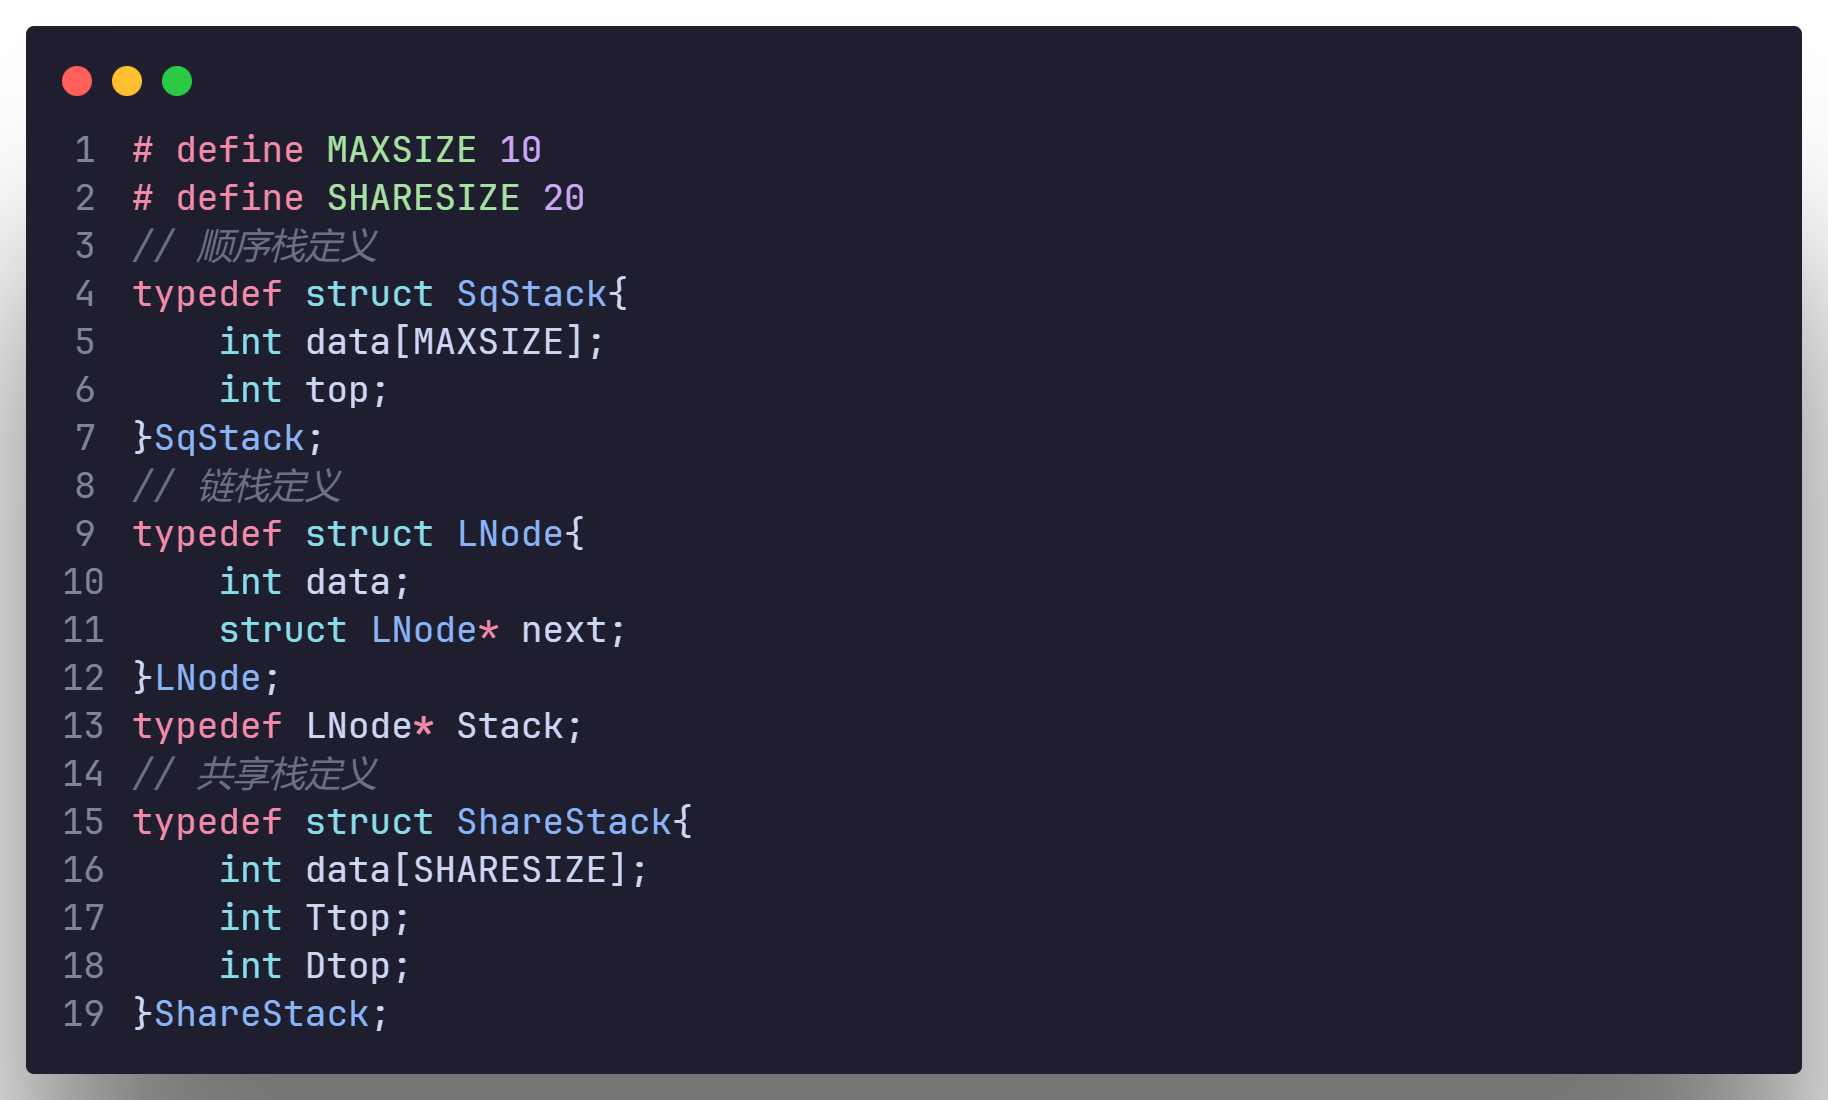
\includegraphics[scale=0.2]{"figure/Note/Stack/SDefine.png"}
\end{figure}

\subsubsection{函数声明}

\begin{figure}[H]
    \centering
    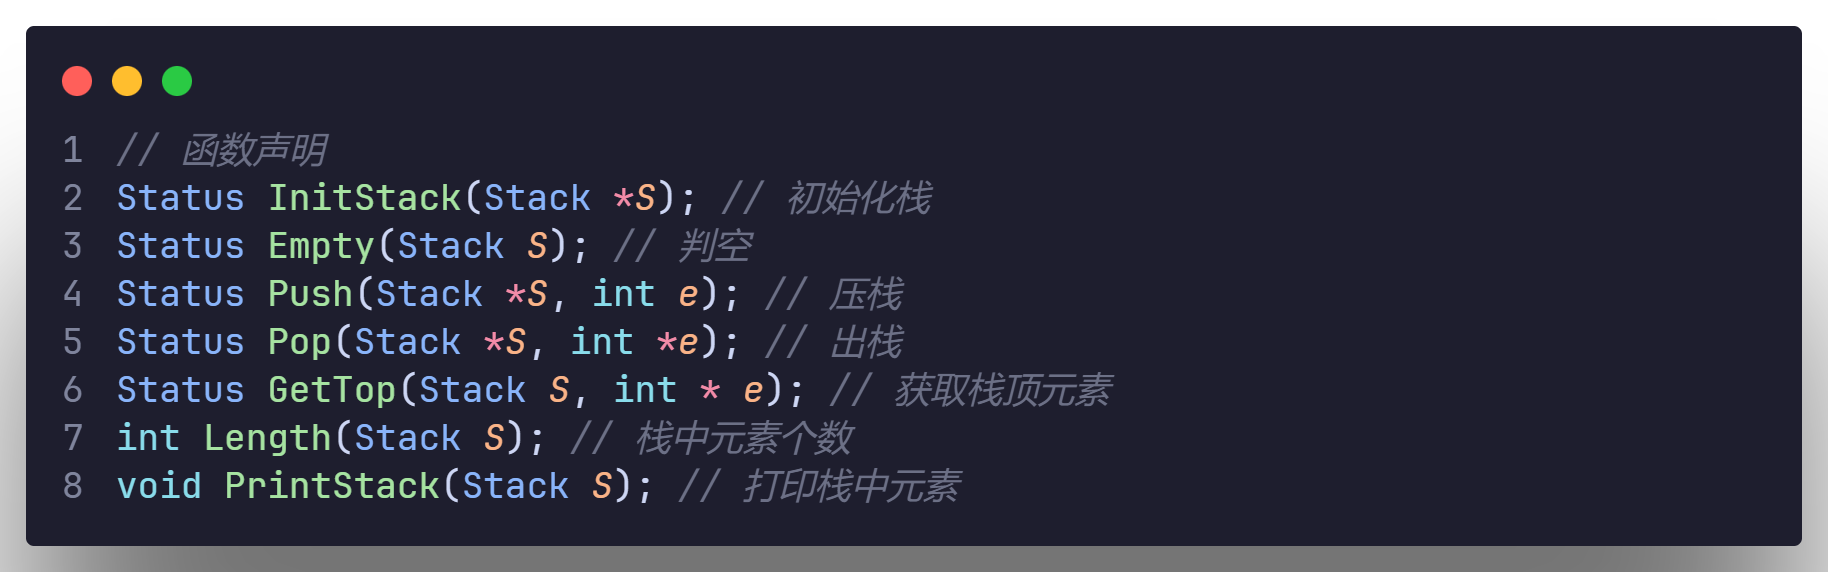
\includegraphics[scale=0.2]{"figure/Note/Stack/SFunction.png"}
\end{figure}

\subsection{顺序栈}
\begin{definition}[顺序栈]
    顺序栈是用顺序表实现的栈,使用 $\mathbf{top}$ 指针指定栈顶元素在顺序表中的位置,栈的容量大小固定, 需要判空和判满.
\end{definition}

\subsubsection{顺序栈初始化}

\begin{figure}[H]
    \centering
    \includegraphics[scale=0.2]{"figure/Note/Stack/SqInit.png"}
\end{figure}

\subsubsection{顺序栈出入栈}

\begin{figure}[H]
    \centering
    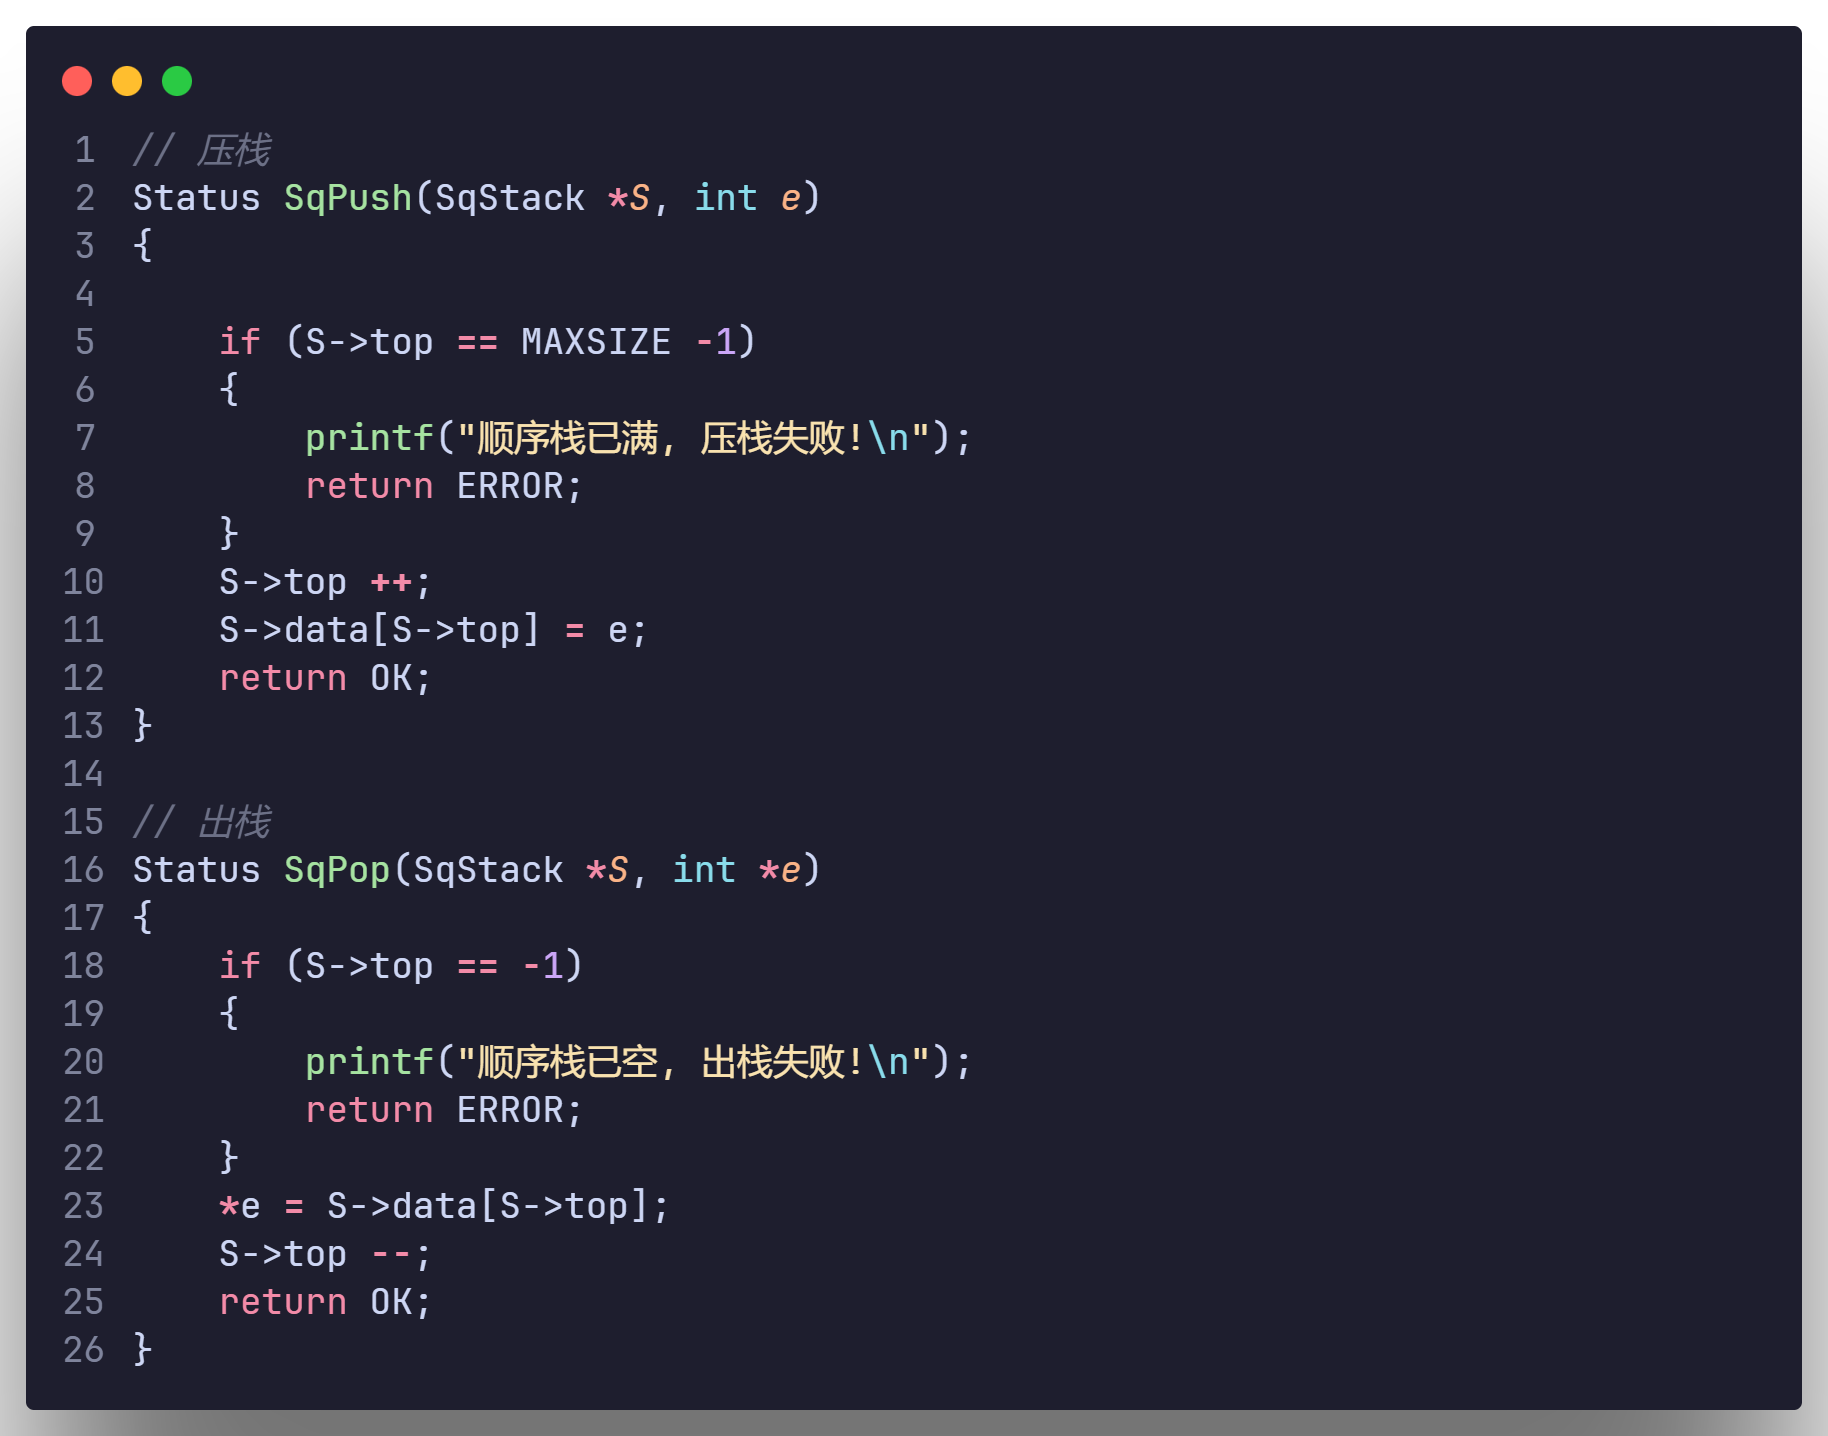
\includegraphics[scale=0.2]{"figure/Note/Stack/SqP.png"}
\end{figure}

\subsubsection{顺序栈辅助函数}

(1). 判断栈是否为空

\begin{figure}[H]
    \centering
    \includegraphics[scale=0.2]{"figure/Note/Stack/SqEmpty.png"}
\end{figure}

(2). 获取栈顶元素

\begin{figure}[H]
    \centering
    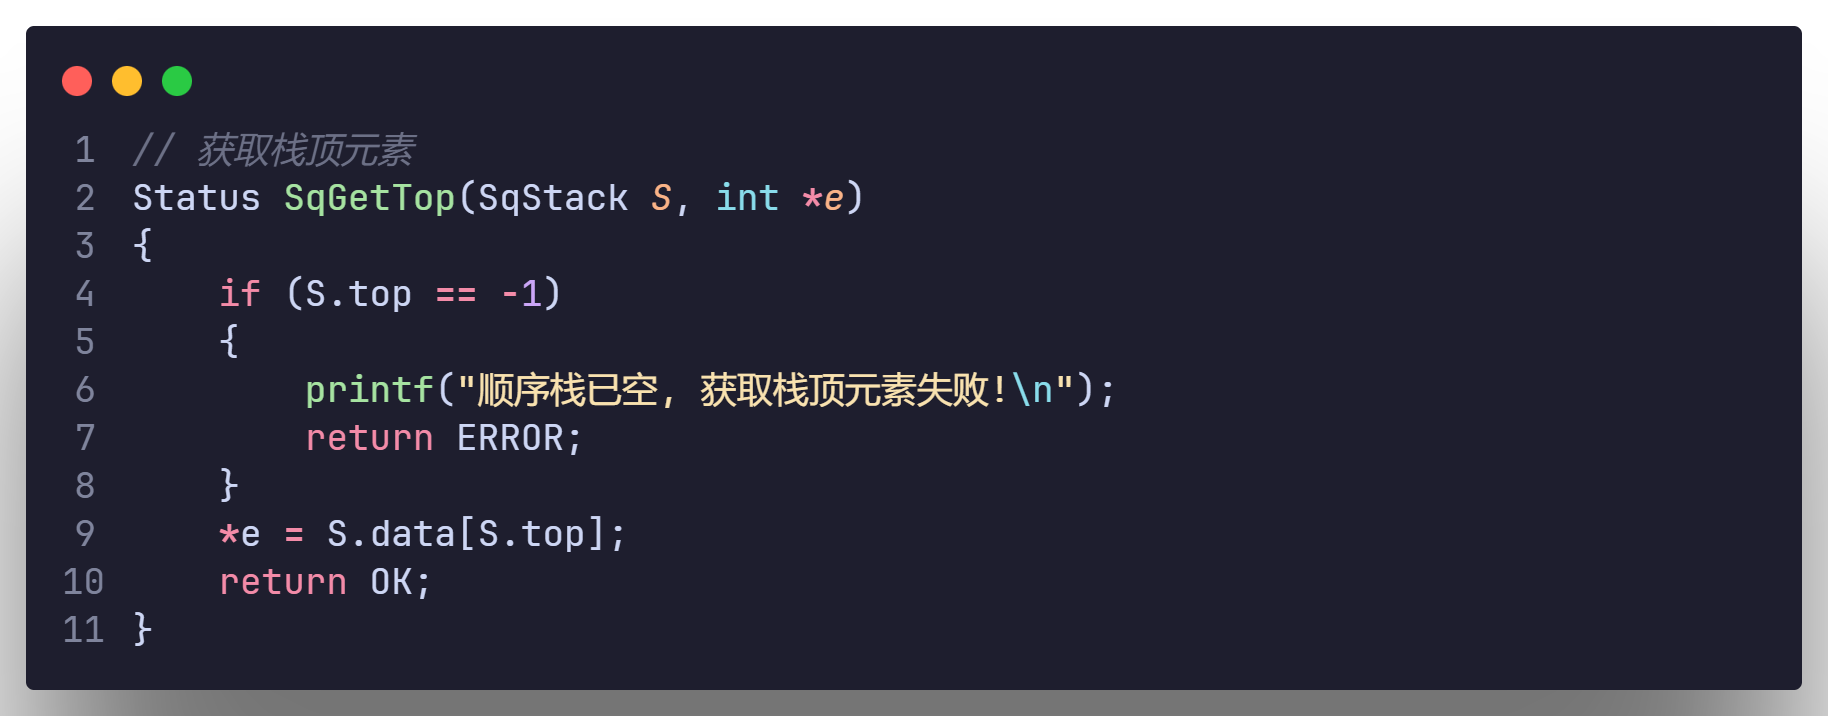
\includegraphics[scale=0.2]{"figure/Note/Stack/SqG.png"}
\end{figure}

(3). 获取栈中元素个数

\begin{figure}[H]
    \centering
    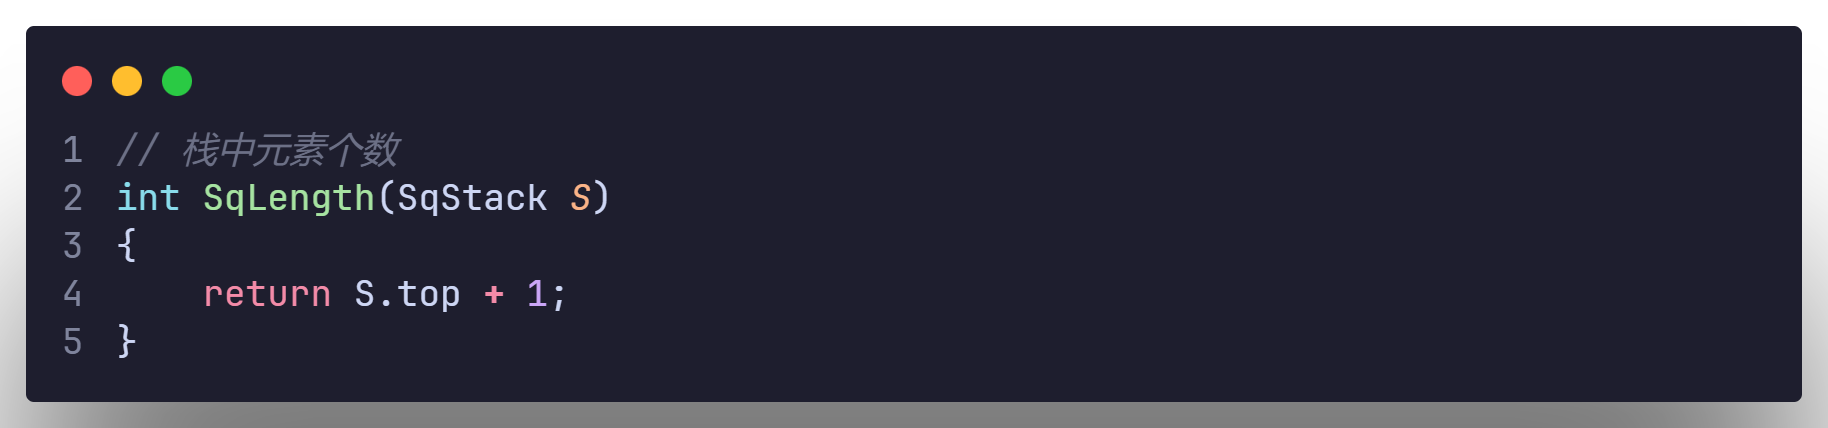
\includegraphics[scale=0.2]{"figure/Note/Stack/SqN.png"}
\end{figure}

(4). 打印栈中元素

\begin{figure}[H]
    \centering
    \includegraphics[scale=0.2]{"figure/Note/Stack/SqPrint.png"}
\end{figure}

\subsection{链栈}
\begin{definition}[链栈]
    链栈是使用链表实现的栈,不需要判满,只需要判空,出栈和入栈操作都在链表的头部进行,只需要表头指针,一般使用不带头节点的单链表实现.
\end{definition}

\subsubsection{链栈初始化}

\begin{figure}[H]
    \centering
    \includegraphics[scale=0.2]{"figure/Note/Stack/SlInit.png"}
\end{figure}

\subsubsection{链栈出入栈}

\begin{figure}[H]
    \centering
    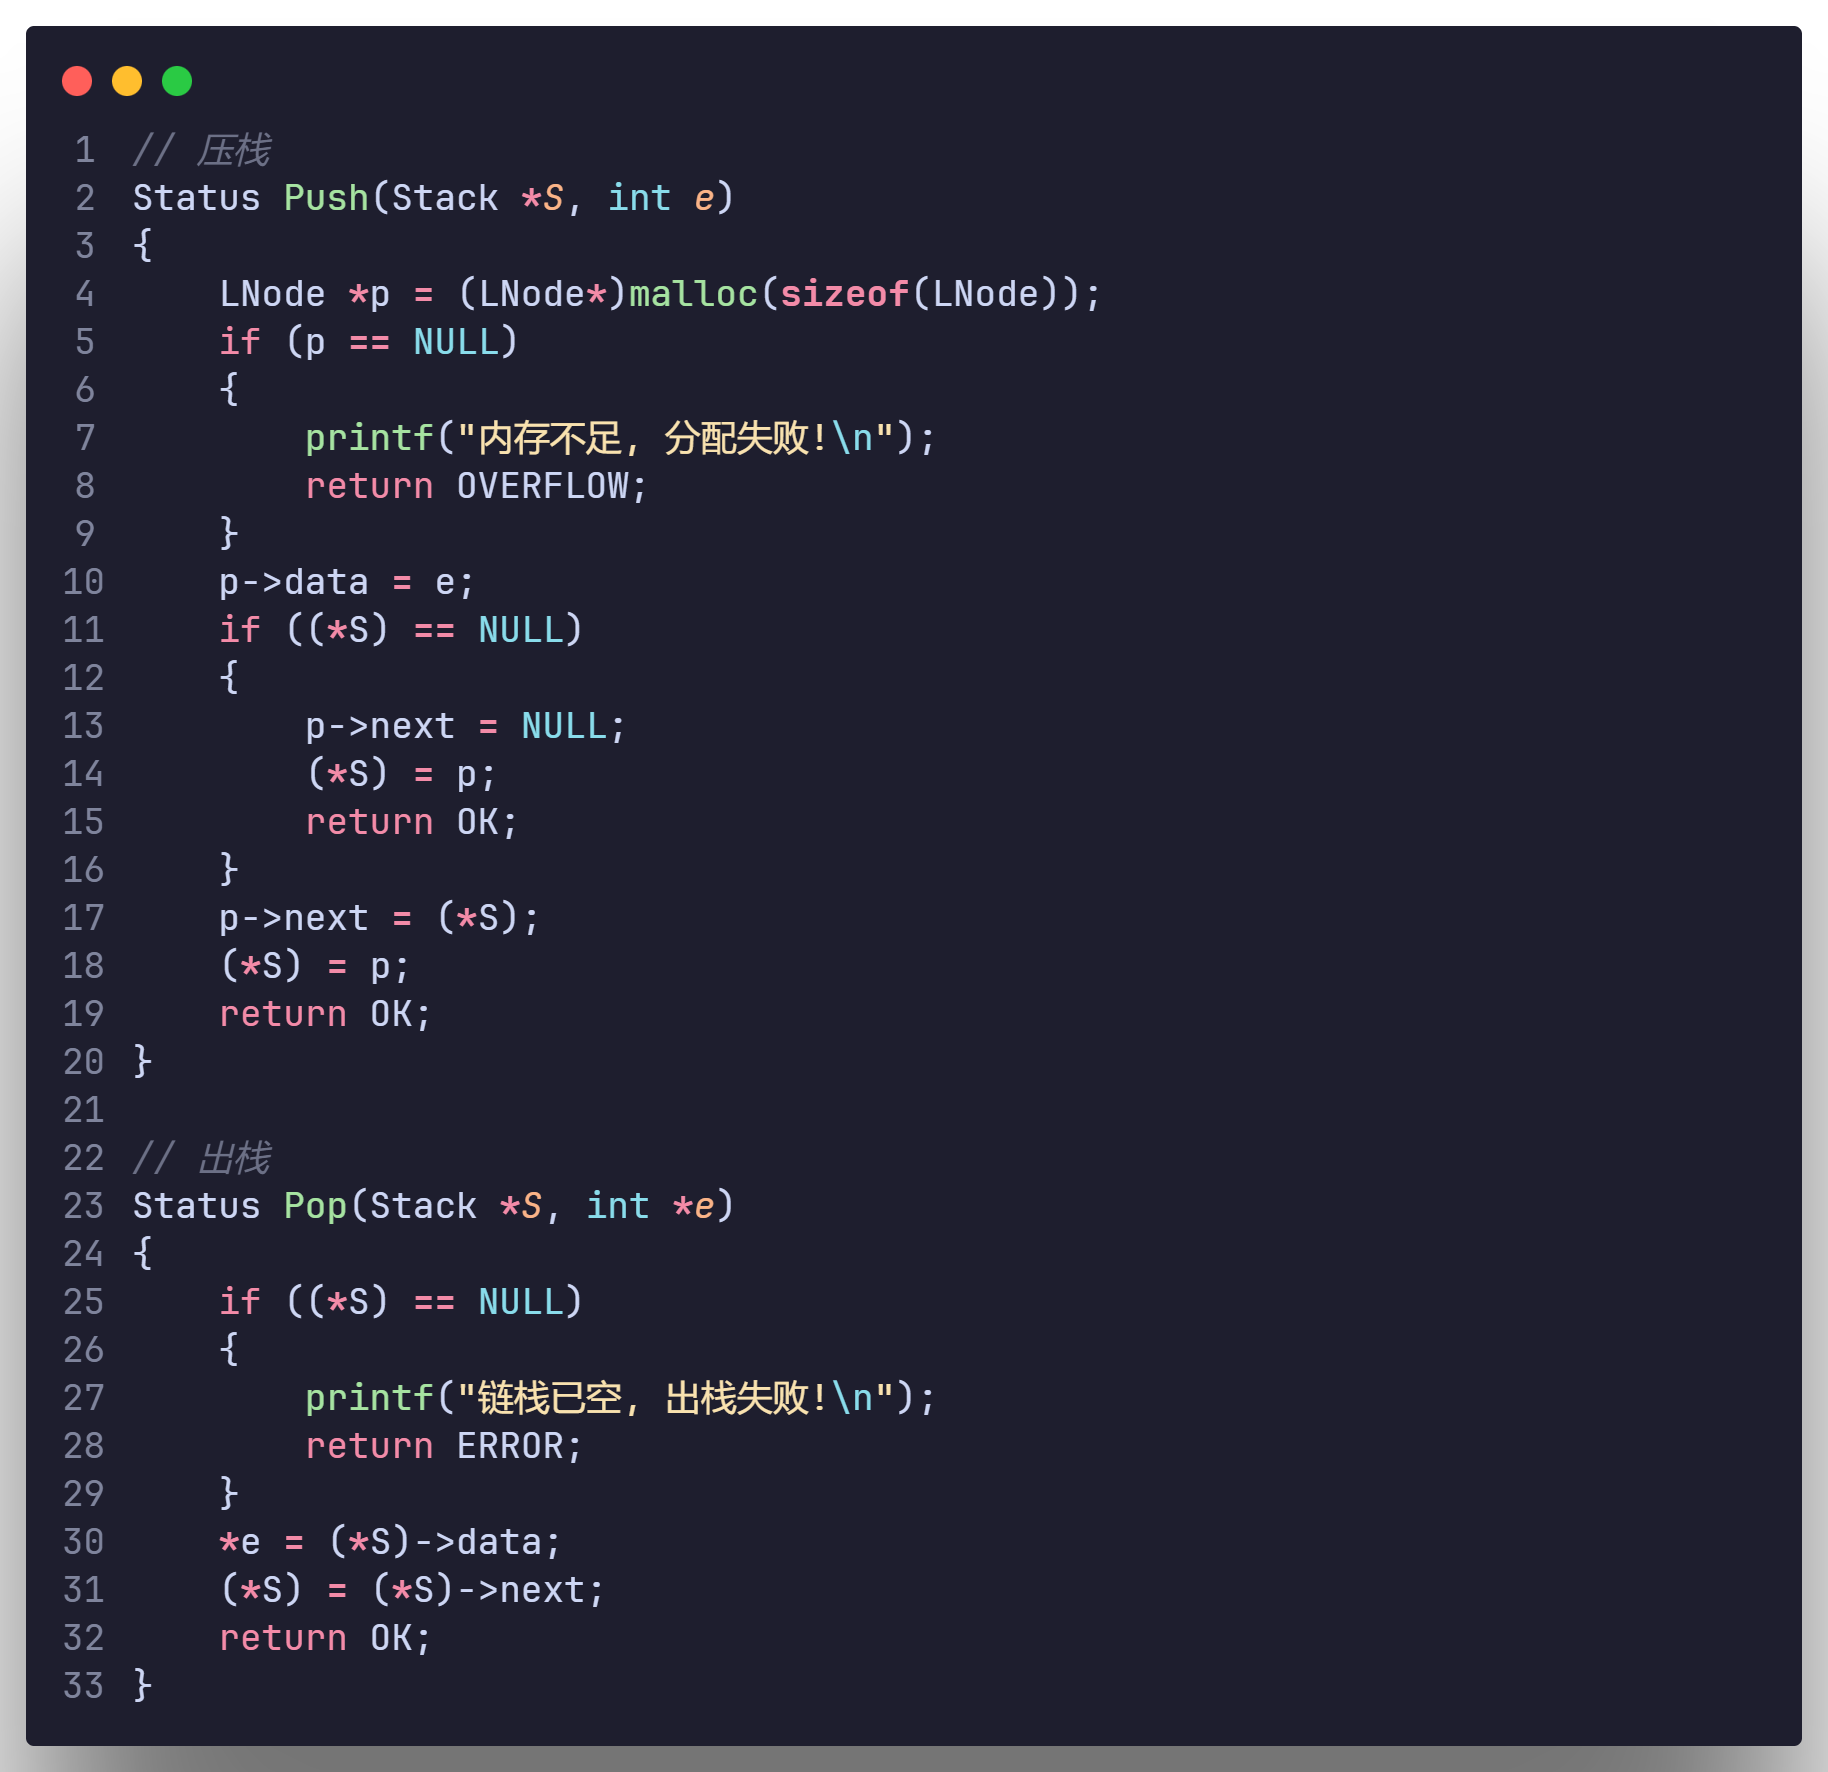
\includegraphics[scale=0.2]{"figure/Note/Stack/SlP.png"}
\end{figure}

\subsubsection{链栈辅助函数}

(1). 判断栈是否为空

\begin{figure}[H]
    \centering
    \includegraphics[scale=0.2]{"figure/Note/Stack/SlEmpty.png"}
\end{figure}

(2). 获取栈顶元素

\begin{figure}[H]
    \centering
    \includegraphics[scale=0.2]{"figure/Note/Stack/SlG.png"}
\end{figure}

(3). 获取栈中元素个数

\begin{figure}[H]
    \centering
    \includegraphics[scale=0.2]{"figure/Note/Stack/SlN.png"}
\end{figure}

(4). 打印栈中元素

\begin{figure}[H]
    \centering
    \includegraphics[scale=0.2]{"figure/Note/Stack/SlPrint.png"}
\end{figure}


\subsection{共享栈}
\begin{definition}[共享栈]
    共享栈是两个栈共享一个顺序表,两个栈的栈底分别在顺序表的两端,两个栈的栈顶指针分别向中间移动,当两个栈的栈顶指针相遇时,表示栈满; 共享栈主要是为了充分利用空间,提高空间利用率.
\end{definition}

\subsubsection{共享栈初始化}

\begin{figure}[H]
    \centering
    \includegraphics[scale=0.2]{"figure/Note/Stack/SSInit.png"}
\end{figure}

\subsubsection{共享栈出入栈}

(1). 入栈

\begin{figure}[H]
    \centering
    \includegraphics[scale=0.2]{"figure/Note/Stack/SSPush.png"}
\end{figure}

(2). 出栈

\begin{figure}[H]
    \centering
    \includegraphics[scale=0.2]{"figure/Note/Stack/SSPop.png"}
\end{figure}

\subsubsection{共享栈辅助函数}

(1). 判断栈是否为空

\begin{figure}[H]
    \centering
    \includegraphics[scale=0.2]{"figure/Note/Stack/SSEmpty.png"}
\end{figure}

(2). 获取栈顶元素

\begin{figure}[H]
    \centering
    \includegraphics[scale=0.2]{"figure/Note/Stack/SSG.png"}
\end{figure}

(3). 获取栈中元素个数

\begin{figure}[H]
    \centering
    \includegraphics[scale=0.2]{"figure/Note/Stack/SSN.png"}
\end{figure}

(4). 打印栈中元素

\begin{figure}[H]
    \centering
    \includegraphics[scale=0.2]{"figure/Note/Stack/SSPrint.png"}
\end{figure}


\section{队列}
\begin{definition}[队列]
    \begin{enumerate}
        \item 只允许在一端进行插入操作,在另一端进行删除操作的线性表
        \item 队列有队头、队尾两个重要元素,队头元素是最先插入的元素,队尾元素是最后插入的元素
        \item 队列的插入操作叫做入队,队列的删除操作叫做出队
        \item 队列的特点是先进先出,简称 $\mathbf{FIFO}, \mathbf{First\ In\ First\ Out}$
    \end{enumerate}
\end{definition}
\begin{definition}[特殊队列]
    1. 循环队列: 顺序表实现的队列,解决顺序表的假溢出问题

    2. 双端队列: 两端都可以进行插入和删除操作的队列

    3. 操作受限的双端队列: 两端都可以进行插入和删除操作,但是有限制,比如只有一端可以插入或者删除
\end{definition}

\begin{definition}[队列基本操作]
    \begin{enumerate}
        \item $\mathbf{InitQueue(\& Q)}$  初始化队列 $Q$
        \item $\mathbf{DestroyQueue(\& Q)}$  销毁队列 $Q$
        \item $\mathbf{GetHead(Q,\&e)}$ 获取队首元素,将队列 $Q$ 队首元素赋值给 $e$
        \item $\mathbf{EnQueue(\&S,e)}$ 入队
        \item $\mathbf{DeQueue(\&S,\&e)}$ 出队
        \item $\mathbf{Length(Q)}$ 求队列中元素个数
        \item $\mathbf{Empty(Q)}$ 判空
        \item $\mathbf{PrintQueue(S)}$ 输出操作,输出队列 $Q$ 的所有元素 
    \end{enumerate}
\end{definition}
\subsection{队列定义和函数声明}
\subsubsection{循环队列、链表队列定义}

\begin{figure}[H]
    \centering
    \includegraphics[scale=0.2]{"figure/Note/Stack/QDefine.png"}
\end{figure}

\subsubsection{函数声明}

\begin{figure}[H]
    \centering
    \includegraphics[scale=0.2]{"figure/Note/Stack/QFunction.png"}
\end{figure}

\subsection{循环队列}
\begin{definition}[循环队列]
    循环队列是使用顺序表实现的队列,为防止出现假溢出,将顺序表的首尾相连,当队尾指针指向顺序表的最后一个位置时,再插入元素时,将队尾指针指向顺序表的第一个位置.

    \textbf{实现方法:}
    \begin{enumerate}
        \item 队列最后一个位置不存储元素,队列中元素个数最多为 $MAXSIZE-1$, 队列满的条件是 $(Q.rear+1)\% MAXSIZE == Q.font$, 队列空的条件是 $Q.rear == Q.font$
        \item 设置一个标志位 $\mathbf{flag}$, 如果 $flag = 0$, 表示上一次是入队操作, 如果 $flag = 1$, 表示上一次是出队操作, 当 $Q.rear == Q.font$ 时, 根据 $flag$ 的值判断是队列满还是队列空, 如果 $flag = 0$, 队列满, 如果 $flag = 1$, 队列空
    \end{enumerate}
\end{definition}
\subsubsection{循环队列初始化}

\begin{figure}[H]
    \centering
    \includegraphics[scale=0.2]{"figure/Note/Stack/QInit.png"}
\end{figure}

\subsubsection{循环队列出入队}

(1). 入队

\begin{figure}[H]
    \centering
    \includegraphics[scale=0.2]{"figure/Note/Stack/QEq.png"}
\end{figure}

(2). 出队

\begin{figure}[H]
    \centering
    \includegraphics[scale=0.2]{"figure/Note/Stack/QDq.png"}
\end{figure}

\subsubsection{循环队列辅助函数}
(1). 获取队首元素

\begin{figure}[H]
    \centering
    \includegraphics[scale=0.2]{"figure/Note/Stack/QG.png"}
\end{figure}

(2). 队列长度

\begin{figure}[H]
    \centering
    \includegraphics[scale=0.2]{"figure/Note/Stack/QLen.png"}
\end{figure}

(3). 判断队列是否为空

\begin{figure}[H]
    \centering
    \includegraphics[scale=0.2]{"figure/Note/Stack/QEmpty.png"}
\end{figure}

(4). 打印队列

\begin{figure}[H]
    \centering
    \includegraphics[scale=0.2]{"figure/Note/Stack/QPrint.png"}
\end{figure}

\subsection{链队列}
\begin{definition}[链队列]
    链队列是使用链表实现的队列,只需要存储队头节点和队尾节点的指针.

    \textbf{实现方法:}
    \begin{enumerate}
        \item 队列入队, 将新节点作为队尾节点的后继节点, 队尾节点变为新节点
        \item 队列出队, 将队头节点作为出队节点, 队头节点变为其后继节点, 释放队头节点的空间
    \end{enumerate}
\end{definition}
\subsubsection{链队列初始化}

\begin{figure}[H]
    \centering
    \includegraphics[scale=0.2]{"figure/Note/Stack/QlInit.png"}
\end{figure}

\subsubsection{链队列出入队}

(1). 入队

\begin{figure}[H]
    \centering
    \includegraphics[scale=0.2]{"figure/Note/Stack/QlEq.png"}
\end{figure}

(2). 出队

\begin{figure}[H]
    \centering
    \includegraphics[scale=0.2]{"figure/Note/Stack/QlDq.png"}
\end{figure}

\subsubsection{链队列辅助函数}
(1). 获取队首元素

\begin{figure}[H]
    \centering
    \includegraphics[scale=0.2]{"figure/Note/Stack/QlG.png"}
\end{figure}

(2). 队列长度

\begin{figure}[H]
    \centering
    \includegraphics[scale=0.2]{"figure/Note/Stack/QlLen.png"}
\end{figure}

(3). 判断队列是否为空

\begin{figure}[H]
    \centering
    \includegraphics[scale=0.2]{"figure/Note/Stack/QlEmpty.png"}
\end{figure}

(4). 打印队列

\begin{figure}[H]
    \centering
    \includegraphics[scale=0.2]{"figure/Note/Stack/QlPrint.png"}
\end{figure}

\subsection{双端队列}
\begin{definition}[双端队列]
    双端队列是两端都能够插入和删除的队列, 一般采用链表或者顺序表实现, 只需要存储队头节点和队尾节点的指针

    \textbf{操作受限的双端队列:}
    \begin{enumerate}
        \item 只有一端可以插入, 两端可以删除的队列
        \item 只有一端可以删除, 两段可以插入的队列
    \end{enumerate}
\end{definition}
\section{栈和队列的应用}
\subsection{括号匹配}
\begin{theorem}[算法步骤]
    \begin{enumerate}
        \item 遇到左括号压栈, 遇到右括号出栈
        \item 如果出栈为空, 或者出栈元素和当前右括号不匹配, 返回错误
        \item 如果遍历完所有括号, 栈为空, 返回正确
    \end{enumerate}
\end{theorem}
\subsection{前缀、中缀、后缀表达式求值}
\begin{theorem}[表达式求值]
    一、前缀表达式: 运算符在前, 操作数在后
    \begin{enumerate}
        \item 从右向左扫描表达式, 遇到操作数入栈, 遇到运算符, 从栈中弹出两个操作数, 进行运算
        \item 第一个弹出的操作数是右操作数, 第二个弹出的操作数是左操作数, 运算结果入栈
        \item 最后栈中的元素就是表达式的值
    \end{enumerate}

    二、中缀表达式: 运算符在中间, 操作数在两边, 直接计算

    三、后缀表达式: 运算符在后, 操作数在前
    \begin{enumerate}
        \item 从左向右扫描表达式, 遇到操作数入栈, 遇到运算符, 从栈中弹出两个操作数, 进行运算
        \item 第一个弹出的操作数是左操作数, 第二个弹出的操作数是右操作数, 运算结果入栈
        \item 最后栈中的元素就是表达式的值
    \end{enumerate}
\end{theorem}

\subsection{表达式转换}
\begin{theorem}[表达式转换: 手算]
    一、中缀表达式 $\to$ 前缀表达式: 按照运算顺序, 从左向右扫描, 把操作符放在左边, 操作数放在右边, 将得到的前缀表达式作为操作数继续进行操作, 直到得到最终的前缀表达式

    二、中缀表达式 $\to$ 后缀表达式: 按照运算顺序, 从左向右扫描, 把操作符放在右边, 操作数放在左边, 将得到的后缀表达式作为操作数继续进行操作, 直到得到最终的后缀表达式

    三、前缀表达式 $\to$ 后缀表达式和 后缀表达式 $\to$ 前缀表达式: 先将前缀表达式转换为中缀表达式, 再将中缀表达式转换为后缀表达式; 同理可以将后缀表达式转换为前缀表达式

\end{theorem}
\subsection{队列应用}
\begin{definition}[队列应用]
    1. 树的层次遍历, 按照根节点入队,出队,再将左右孩子入队,出队,直到队列为空

    2. 图的广度优先搜索, 按照顶点入队,出队,再将与该顶点相邻的顶点入队,出队,直到队列为空

    3. 模拟操作系统的进程调度, 先到的进程先执行,后到的进程后执行($\mathbf{FCFS}$)

    4. 图的深度有限搜索, 按照顶点入栈,出栈,再将与该顶点相邻的顶点入栈,出栈,直到栈为空
\end{definition}

\section{数组}
\begin{definition}[数组]
    数组是由类型相同的元素构成的有序集合, 每个元素称为数组元素, 每个元素有唯一下标, 可通过下标访问该数据元素; 
    一维数组可以看作线性表; 二维数组是数据元素为一维数组的线性表
\end{definition}
$$LOC(i,j) = LOC(0,0) + (n\times i + j)L$$

\subsection{特殊矩阵的压缩}
\subsubsection{对称矩阵}

$a_{ij}$ 在数组中的下标 $k$

$$ k =
\begin{cases}
    \dfrac{i(i-1)}{2}+j-1, & i\geq j\\
    \dfrac{j(j-1)}{2}+i-1, & i<j\ (a_{ij}=a_{ji})
\end{cases}
$$

\subsubsection{三角矩阵}

(1). 上三角矩阵

$a_{ij}$在数组中的下标$k$:

$$ k = 
\begin{cases}
    \dfrac{(i-1)(2n-i+2)}{2}+j-i, & i\leq j\\
    \dfrac{n(n+1)}{2},            & i > j\ (a_{ij}=c)
\end{cases}
$$

(2). 下三角矩阵

$a_{ij}$在数组中的下标$k$:

$$ k = 
\begin{cases}
    \dfrac{i(i-1)}{2}+j-1, & i\geq j\\
    \dfrac{n(n+1)}{2},     & i < j\ (a_{ij}=c)
\end{cases}
$$

\subsubsection{对称矩阵}

(1). 三对角矩阵

$a_{ij}$ 在数组中的下标 $k$:

$$ k = 
\begin{cases}
    2i+j-3, & |i-j| \leq 1\\
    3n-2,   & |i-j| > 1
\end{cases}
$$

已知数组下标 $k$ 时:

$$\begin{cases}
    i = [\dfrac{k+1}{3}]+1\\
    j = k-2i+3
\end{cases}$$

\subsubsection{稀疏矩阵}

采用三元组的方式存储, 不仅需要存储数据, 还需要存储行号和列号以及非零元素的个数, 失去随机存储的特性
\begin{table}[ht]
    \centering
    \begin{tabular}{>{\centering\arraybackslash}p{1cm} >{\centering\arraybackslash}p{1cm} >{\centering\arraybackslash}p{2cm}}
    \toprule
    \rowcolor[HTML]{FCE5CD} 
    \textit{i} & \textit{j} & \textit{num} \\ 
    \midrule
    \rowcolor[HTML]{FFF2CC} 
    0 & 0 & 4 \\ 
    \rowcolor[HTML]{FCE5CD} 
    1 & 2 & 6 \\ 
    \rowcolor[HTML]{FFF2CC} 
    2 & 1 & 9 \\ 
    \rowcolor[HTML]{FCE5CD} 
    3 & 1 & 23 \\ 
    \bottomrule
    \end{tabular}
\end{table}

\section{栈和队列可视化}
\begin{enumerate}
    \item \href{https://www.cs.usfca.edu/~galles/visualization/StackArray.html}{数组栈}
    \item \href{https://www.cs.usfca.edu/~galles/visualization/StackLL.html}{链表栈}
    \item \href{https://www.cs.usfca.edu/~galles/visualization/QueueArray.html}{数组队列}
    \item \href{https://www.cs.usfca.edu/~galles/visualization/QueueLL.html}{链表队列}
\end{enumerate}
	%\input{chap/3.串.tex}
	%\chapterimage{chap5.jpg}
\chapter{树和森林}

\section{树的基本概念}

\begin{forest}
    for tree={
        circle, draw, minimum size=1cm,l=1.5cm, 
        edge={thick,->},
        where level=0{fill=red}{},
        where level=1{fill=purple}{},
        where level=2{fill=green}{},
        where level=3{fill=yellow}{}
    }
    [A
      [B
        [E
          [K]
          [L]
        ]
        [F]
      ]
      [C
        [G]
      ]
      [D
        [H
          [M]
        ]
        [I]
        [J]
      ]
    ]
\end{forest}
\section{二叉树}
\begin{forest}
    for tree={
        circle, draw, minimum size=1cm, inner sep=0pt, s sep=1cm, l=1.5cm, 
        edge={thick,->},
        where level=0{fill=red}{},
        where level=1{fill=blue}{},
        where level=2{fill=green}{}
    }
    [A
      [B
        [D]
        [E]
      ]
      [C
        [F]
        [G]
      ]
    ]
\end{forest}
\section{二叉树遍历和线索二叉树}
	%\input{chap/5.图.tex}
	%\input{chap/6.查找.tex}
	%\input{chap/7.排序.tex}
\end{document}